\documentclass{mcmthesis}
\mcmsetup{
	CTeX = false,
	tcn = {2504496},
	problem = \textcolor{red}{A},
	sheet = true,
	titleinsheet = true,
	keywordsinsheet = true,
	titlepage = false,
	abstract = false
}

\usepackage{tcolorbox}
\usepackage{xcolor}
\usepackage{enumitem}
\usepackage{adjustbox} % 在导言区添加
\definecolor{customblue}{RGB}{165,216,255} % 定义 #a5d8ff 的 RGB 值
\definecolor{deepblue}{RGB}{0,74,173}      % 配套深蓝色

% ================ 环境定义 ================
\newenvironment{featurebox}[1]{%
	\begin{tcolorbox}[
		colback=white,                  % 白色背景
		colframe=customblue,            % 边框颜色 #a5d8ff
		colbacktitle=customblue,        % 标题背景色
		coltitle=deepblue,              % 标题文字颜色
		arc=3mm,                        % 圆角半径
		boxrule=1.5pt,                  % 边框粗细
		title={\large\bfseries #1},     % 标题内容
		fonttitle=\sffamily,            % 无衬线字体
		top=10pt,                       % 上边距
		bottom=10pt,                    % 下边距
		left=10pt,                      % 左边距
		right=10pt,                     % 右边距
		]
	}{\end{tcolorbox}}
% ================ 预声明hyperref选项 ================
\PassOptionsToPackage{hyphens}{url}
\PassOptionsToPackage{colorlinks=true, linkcolor=blue, urlcolor=cyan, citecolor=magenta}{hyperref}

% ================ 基础包配置 ================
\usepackage{newtxtext}
\usepackage{amsmath}
\usepackage{graphicx}
\usepackage{tabularx}
\usepackage{array}
\usepackage{booktabs}
\usepackage[table,xcdraw]{xcolor}

% ================ 算法排版包 ================
\usepackage{algorithm}
\usepackage{algpseudocode}

% ================ 参考文献配置 ================
\usepackage[style=ieee,backend=biber]{biblatex}
\addbibresource{reference.bib}

% ================ 目录格式配置 ================
\usepackage{tocloft}
\setlength{\cftbeforesecskip}{6pt}
\renewcommand{\contentsname}{\hspace*{\fill}\Large\bfseries Contents \hspace*{\fill}}

% ================ 页眉页脚配置 ================
\usepackage{fancyhdr}
\setlength{\headheight}{13.6pt}

% ================ 子图表支持 ================
\usepackage{subcaption}

% ================ 最后加载hyperref ================
\usepackage{hyperref} % 必须保持最后加载

% ================ 自定义颜色 ================
\definecolor{lightgray}{RGB}{240,240,240}
\definecolor{lightblue}{RGB}{173,216,230}

% ================ 表格样式配置 ================
\newcolumntype{Y}{>{\raggedright\arraybackslash}X}
\setlength{\arrayrulewidth}{0.5mm}
\setlength{\tabcolsep}{12pt}
\renewcommand{\arraystretch}{1.2}

\title{Enjoy a Cozy and Green Bath}
\date{\today}
\begin{document}
	
	%%%%%%%%%%%%%%%%%%%%%%%%%%%%%%%%%%%%%%%%
	%%%%%%%%%%%%%%%%% 摘要 %%%%%%%%%%%%%%%%%
	%%%%%%%%%%%%%%%%%%%%%%%%%%%%%%%%%%%%%%%%
	\begin{abstract}
		
		abstract...
		
		\begin{keywords}
			Keyword one, Keyword two, Keyword three
		\end{keywords}
		
	\end{abstract}
	
	
	\maketitle
	\tableofcontents        % 若不想要目录, 注释掉该句
	\thispagestyle{empty}
	\newpage
	
	
	
	
	
	%%%%%%%%%%%%%%%%%%%%%%%%%%%%%%%%%%%%%%%%
	%%%%%%%%%%%%%%%%% 引言 %%%%%%%%%%%%%%%%%
	%%%%%%%%%%%%%%%%%%%%%%%%%%%%%%%%%%%%%%%%
	
	
	\section{Introduction}
	
	\subsection{Background}
	The medal table of the 2024 Paris Olympics shows that the United States and China each won 40 gold medals and tied for the top spot, but the United States led with a total of 126 medals. The host country France ranked fifth in gold medals (16) and fourth in total medals (64). Dominica, Saint Lucia and other countries won their first Olympic medals, while 60 countries still have not broken through for any medals.
	\begin{figure}[htbp]
		\centering
		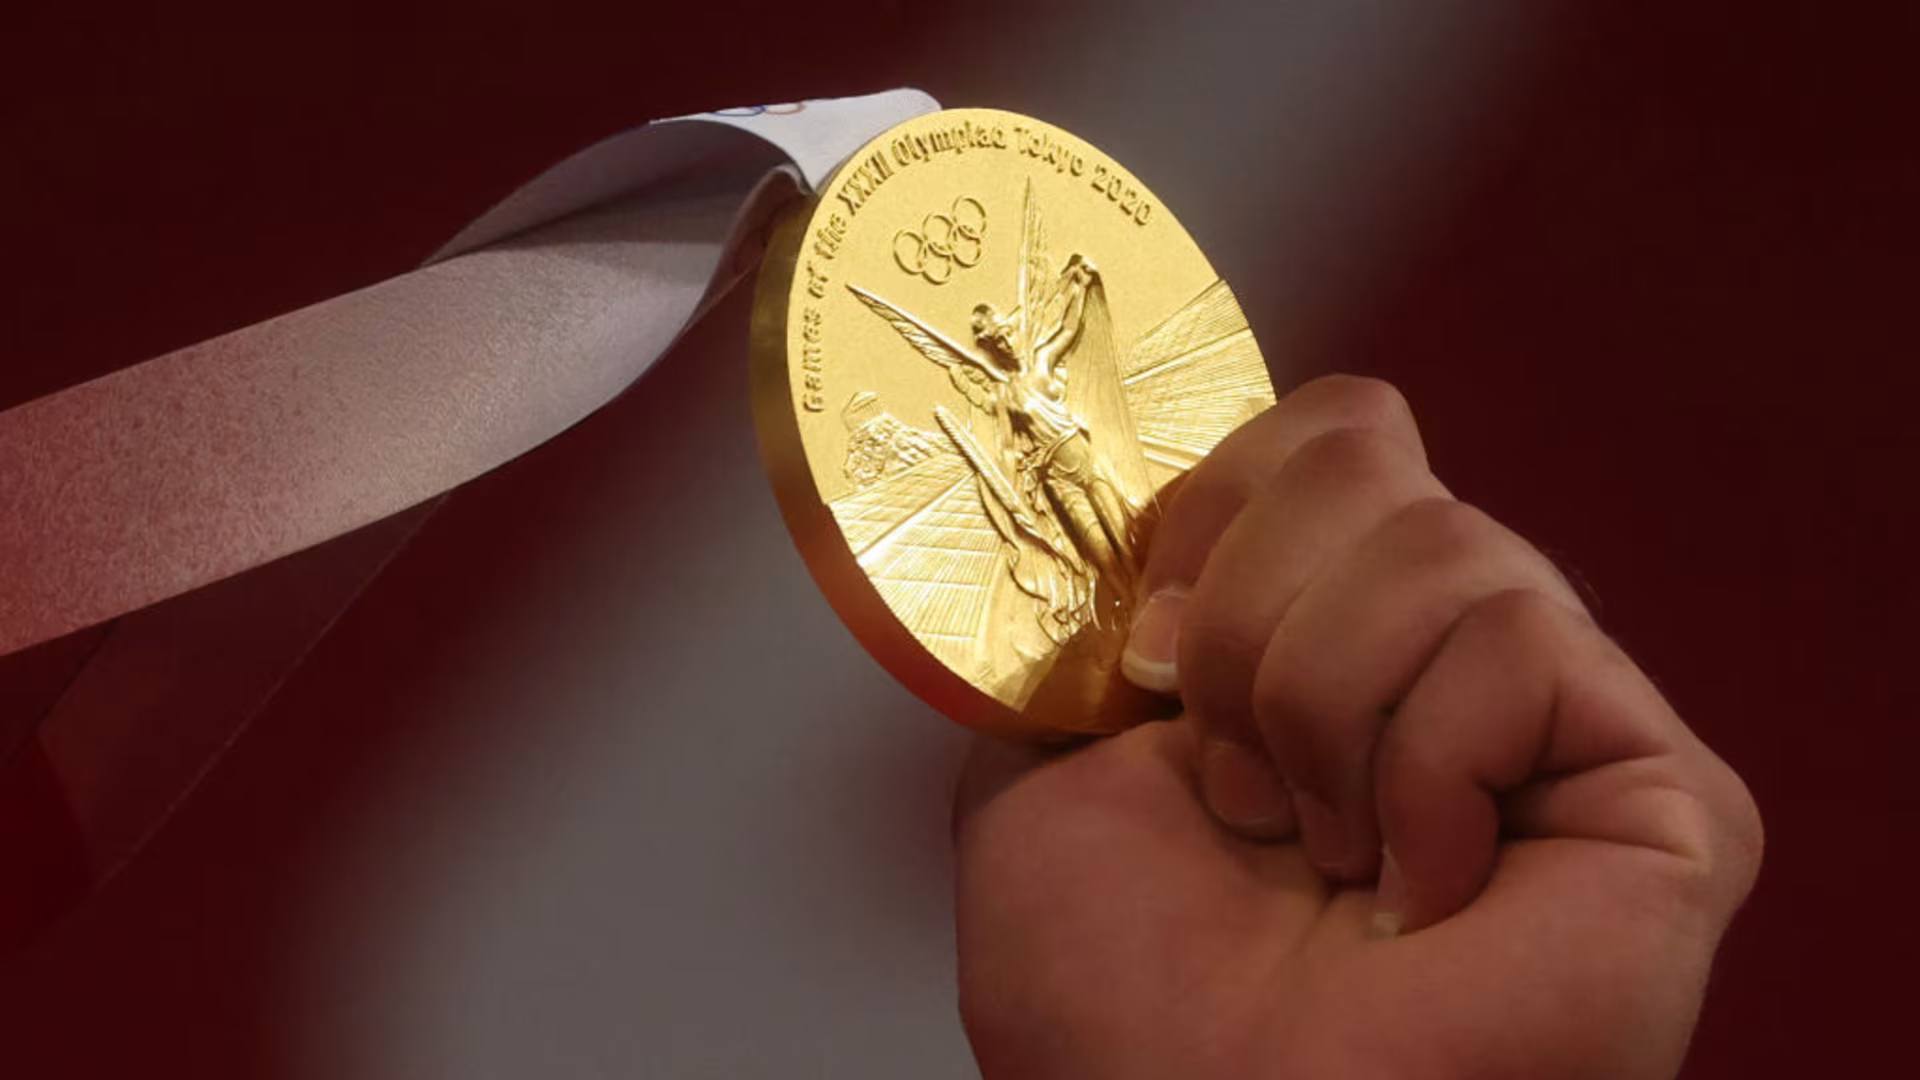
\includegraphics[width=0.7\linewidth]{fig/background}
		\caption{The medals of the 2024 Paris Olympics}
	\end{figure}
	
	\subsection{Restatement and Analysis of the Problem}
	Based on the provided historical data-set of the Olympic Games from 1896 to 2024, we are employed to analyze and answer the following questions:
	\begin{enumerate}
		\item 
		Develop a \textbf{prediction model} to forecast the number of medals each country will win in 2028, and identify countries that may progress or regress. 
		\item 
		Provide \textbf{prediction intervals} and estimates of \textbf{uncertainty} and metrics to measure the model's performance.
		\item 
		Estimate the number of countries that will win their \textbf{first medal} and the probability of this happening.
		\item 
		Analyze the \textbf{relationship} between specific Olympic events (in terms of quantity and type) and the number of medals, explore which events are more important, and the impact of the host country's event selection strategy on the outcome.
		\item 
		Verify whether the \textbf{mobility of coaches} significantly enhances a country's performance in specific sports (such as Lang Ping and Bela Karolyi).
		\item 
		Quantify the contribution of\textbf{ coaching effectiveness} to the number of medals, and recommend key sports for investment and expected returns for the three countries.
		\item 
		Extract the less-attended-to patterns from the model and provide strategic \textbf{suggestions} for the Olympic Committee.
	\end{enumerate}
	
	
	
	%对于Task1,我们选取7个指标,建立了基于LSTM的奖牌数量预测模型,并使用贝叶斯估计给出了区间预测,而对于从未获奖的国家,我们根据新增的event、运动员数量、历史参与趋势,建立了基于SVM的“首奖突破”预测模型。
	%对于Task2,我们分析了“伟大教练”效应的影响。
	
	
	
	
	
	
	
	
	
	\subsection{Overview of Our Work}
		\begin{figure}[H]
		\centering
		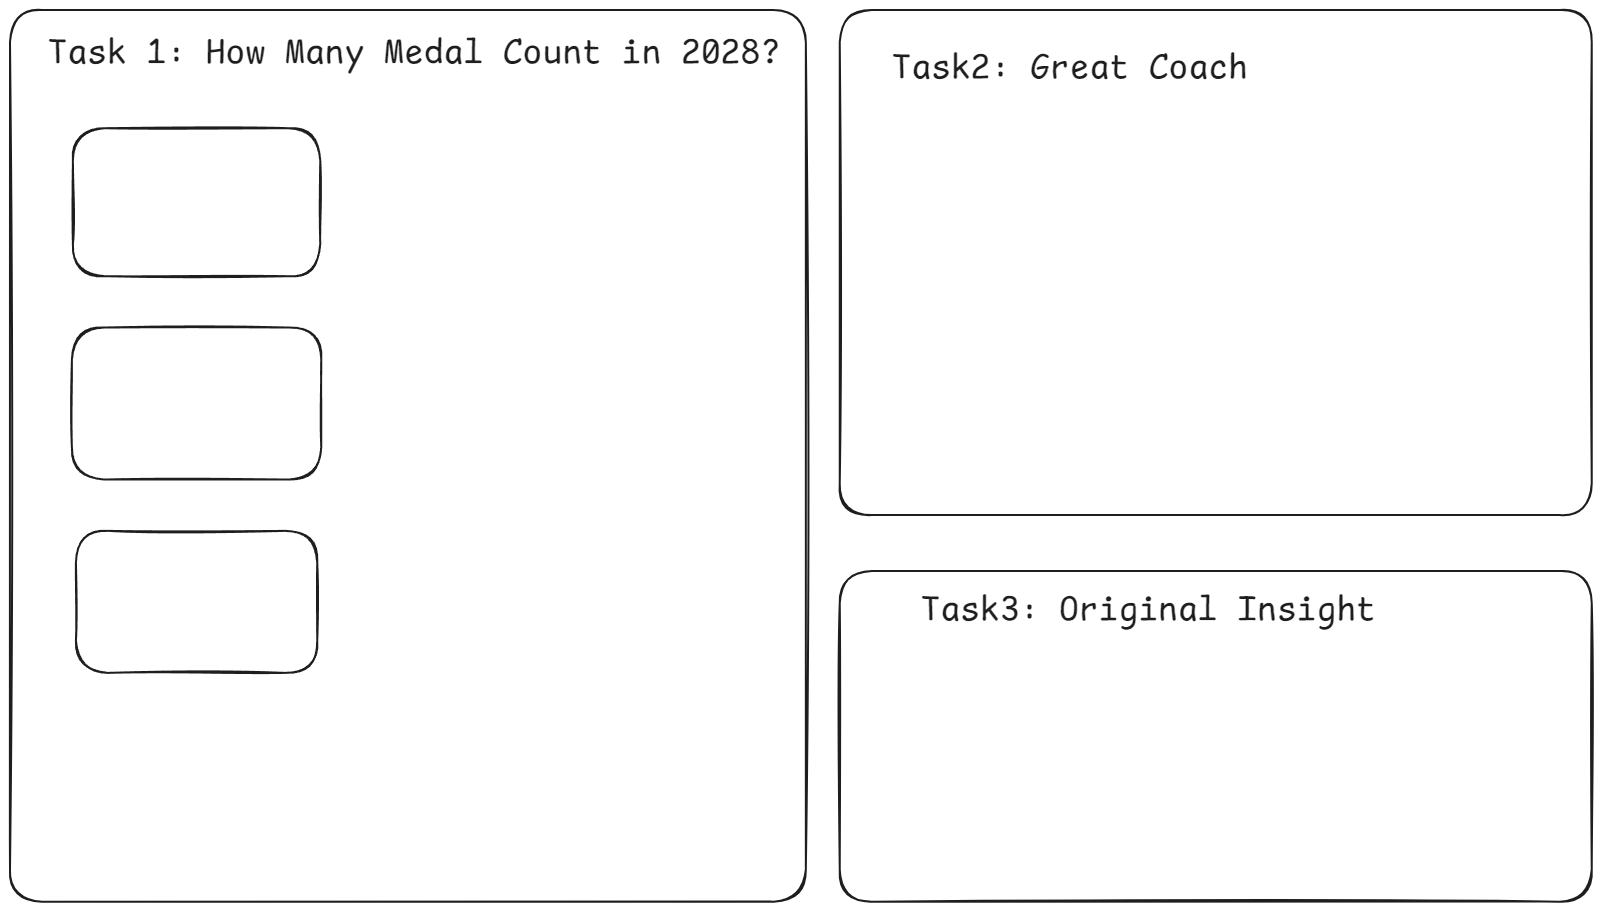
\includegraphics[width=1\linewidth]{fig/1.png}
		\caption{Overview of Our Work}
		\label{fig:Overview of Our Work}
	\end{figure}
	%\begin{itemize}
	%	\item {\bf 111}. ...
	%	\item {\bf 222}. ...
	%	
	%	\begin{itemize}
		%		\item[1)] ... 
		%		\item[2)] ...
		%		\item[3)] ...
		%		\item[4)] ...
		%	\end{itemize}
	%	
	%\end{itemize}
	
	
	
	
	
	
	
	
	%%%%%%%%%%%%%%%%%%%%%%%%%%%%%%%%%%%%%%%%
	%%%%%%%%%%%%%%%%% 模型假设 %%%%%%%%%%%%%%%%%
	%%%%%%%%%%%%%%%%%%%%%%%%%%%%%%%%%%%%%%%%
\section{Assumptions and Justification}

\begin{enumerate}[leftmargin=0.15in, labelsep=0.1in, itemsep=10pt, parsep=5pt]
	\item \textbf{Historical medal data exhibits temporal dependencies that reflect future medal trends. }
	
	This suggests that historical performance can offer insights into future outcomes, and thus, should be treated as a time series when making predictions.
	
	\item \textbf{Monte Carlo Dropout approximates Bayesian inference by quantifying prediction uncertainty through multiple stochastic samplings.}
	
	This technique provides a robust mechanism for estimating confidence intervals and is useful in scenarios with incomplete or noisy data.
	
	\item \textbf{Historical data distributions of non-medal-winning countries align with those of future potential medal-winning nations.} 
	
	This assumption supports the idea that non-medal-winning countries have similar characteristics to those that may perform well in future Olympics, making them a valuable reference for predicting future medal potential.
	
	\item \textbf{The impact of coaching remains independent of confounding variables (e.g., athlete training conditions, changes in international competition rules).} 
	
	This assumption isolates the effect of coaching from other factors that might influence performance, ensuring that coaching effects can be accurately assessed.
\end{enumerate}

	%%%%%%%%%%%%%%%%%%%%%%%%%%%%%%%%%%%%%%%%
	%%%%%%%%%%%%%%%%% 符号说明 %%%%%%%%%%%%%%%%%
	%%%%%%%%%%%%%%%%%%%%%%%%%%%%%%%%%%%%%%%%
\section{List of Notations}
\begin{center}
	\begin{tabular}{ll}
		\toprule
		{\bf Symbols} & {\bf Description}  \\
		\midrule 
		$A_{C},A_{S}$ & Set of country, all sports in Olympic.\\
		$A_{T}$ & $\{1,\dots,30\}$, representing the ordinal number of year Olympic held. \\
		$A_E(j)$ & Represents the set of events inside the sport j.\\
		$A_{H}(t)$ & Set of host country in year $t$. \\
		$MG_{t,i,j,k}$ & Number of gold medals country $i$ won in sport $j$ at event $k$ in year t. \\
		$MS_{t,i,j,k}$ & Number of silver medals country $i$ won in sport $j$ at event $k$ in year t. \\
		$MB_{t,i,j,k}$ & Number of bronze medals country $i$ won in sport $j$ at event $k$ in year t. \\
		$MT_{t,i}$ & Number of total medals country $i$ won in year $t$. \\
		$N_{athletes}(t,i)$ & Total number of athletes from country $i$ in year $t$. \\
		$N_{award}(t,i)$ & Number of athletes who won medals from country $i$ in year $t$. \\
		$H(t,i)$ & Host effect. \\
		$G_{\text{growth}}(t,i)$ & Growth rate of the number of athletes from country $i$ in year $t$.\\
		$P_{Medal}(t,i)$ & Probability of country $i$ winning a medal in year $t$.\\
		$P_{Gold}(t,i)$ & Probability of country $i$ winning a gold medal in year $t$.\\
		\bottomrule
	\end{tabular}
\end{center}

\noindent Note: The Summer Olympics have been held for a total of 32 sessions.
	
	
	
	
	
	
	
	
	
	%%%%%%%%%%%%%%%%%%%%%%%%%%%%%%%%%%%%%%%%
	%%%%%%%%%%%%%%%%% 数据预处理 %%%%%%%%%%%%%%%%%
	%%%%%%%%%%%%%%%%%%%%%%%%%%%%%%%%%%%%%%%%
	\section{Data Pre-processing}
	
	\subsection{Outlier and Missing Value Handling}
	As the \textbf{1906 Intercalated Games} lacked the medal data of various countries and the competition results were not recognized by the International Olympic Committee, the data of 1906 is not taken into account.
	
	In adition, \textbf{Skating} and \textbf{Ice Hockey} have been included in the Winter Olympics since 1920, so these two events are not within the scope of consideration. Otherwise, the "$\cdot$" is replaced by the number $0$. 
	
	It was noticed that \textbf{Jeu de Paume} and \textbf{Roque} sports in the {\bf summerOly\_programs.csv} do not have Codes. Upon researching information from {\color{blue}\url{https://en.wikipedia.org/wiki/Jeu_de_paume}} and {\color{blue}\url{https://en.wikipedia.org/wiki/Roque}}, it was found that only a few people are still engaged in these two sports, which have even not been held for 26 consecutive years in the Summer Olympics. Therefore, these two sports have been excluded.
	
	%\section{Descriptive statistical analysis}
	
	
	
	
	
	
	
	
	
	
	
	
	
	
	
	%%%%%%%%%%%%%%%%%%%%%%%%%%%%%%%%%%%%%%%%
	%%%%%%%%%%%%%%%%% Task 1 %%%%%%%%%%%%%%%%%
	%%%%%%%%%%%%%%%%%%%%%%%%%%%%%%%%%%%%%%%%
	\newpage
	\section{Task 1: How Many Medal Count in 2028? }
	\subsection{Medal-Winning Countries' Medal Count Prediction using LSTM-MCD}
	
	\subsubsection{Significance Analysis of Host Effect}
	
\hspace{1.5em} Host Effect refers to the phenomenon where a host country tends to perform better in large-scale international events (such as the Olympic Games or the World Cup) due to the advantages associated with competing on home soil. This often manifests in a significnt increase in the host country's medal count, competition results, and overall performance.

	\begin{figure}[H]
		\centering
		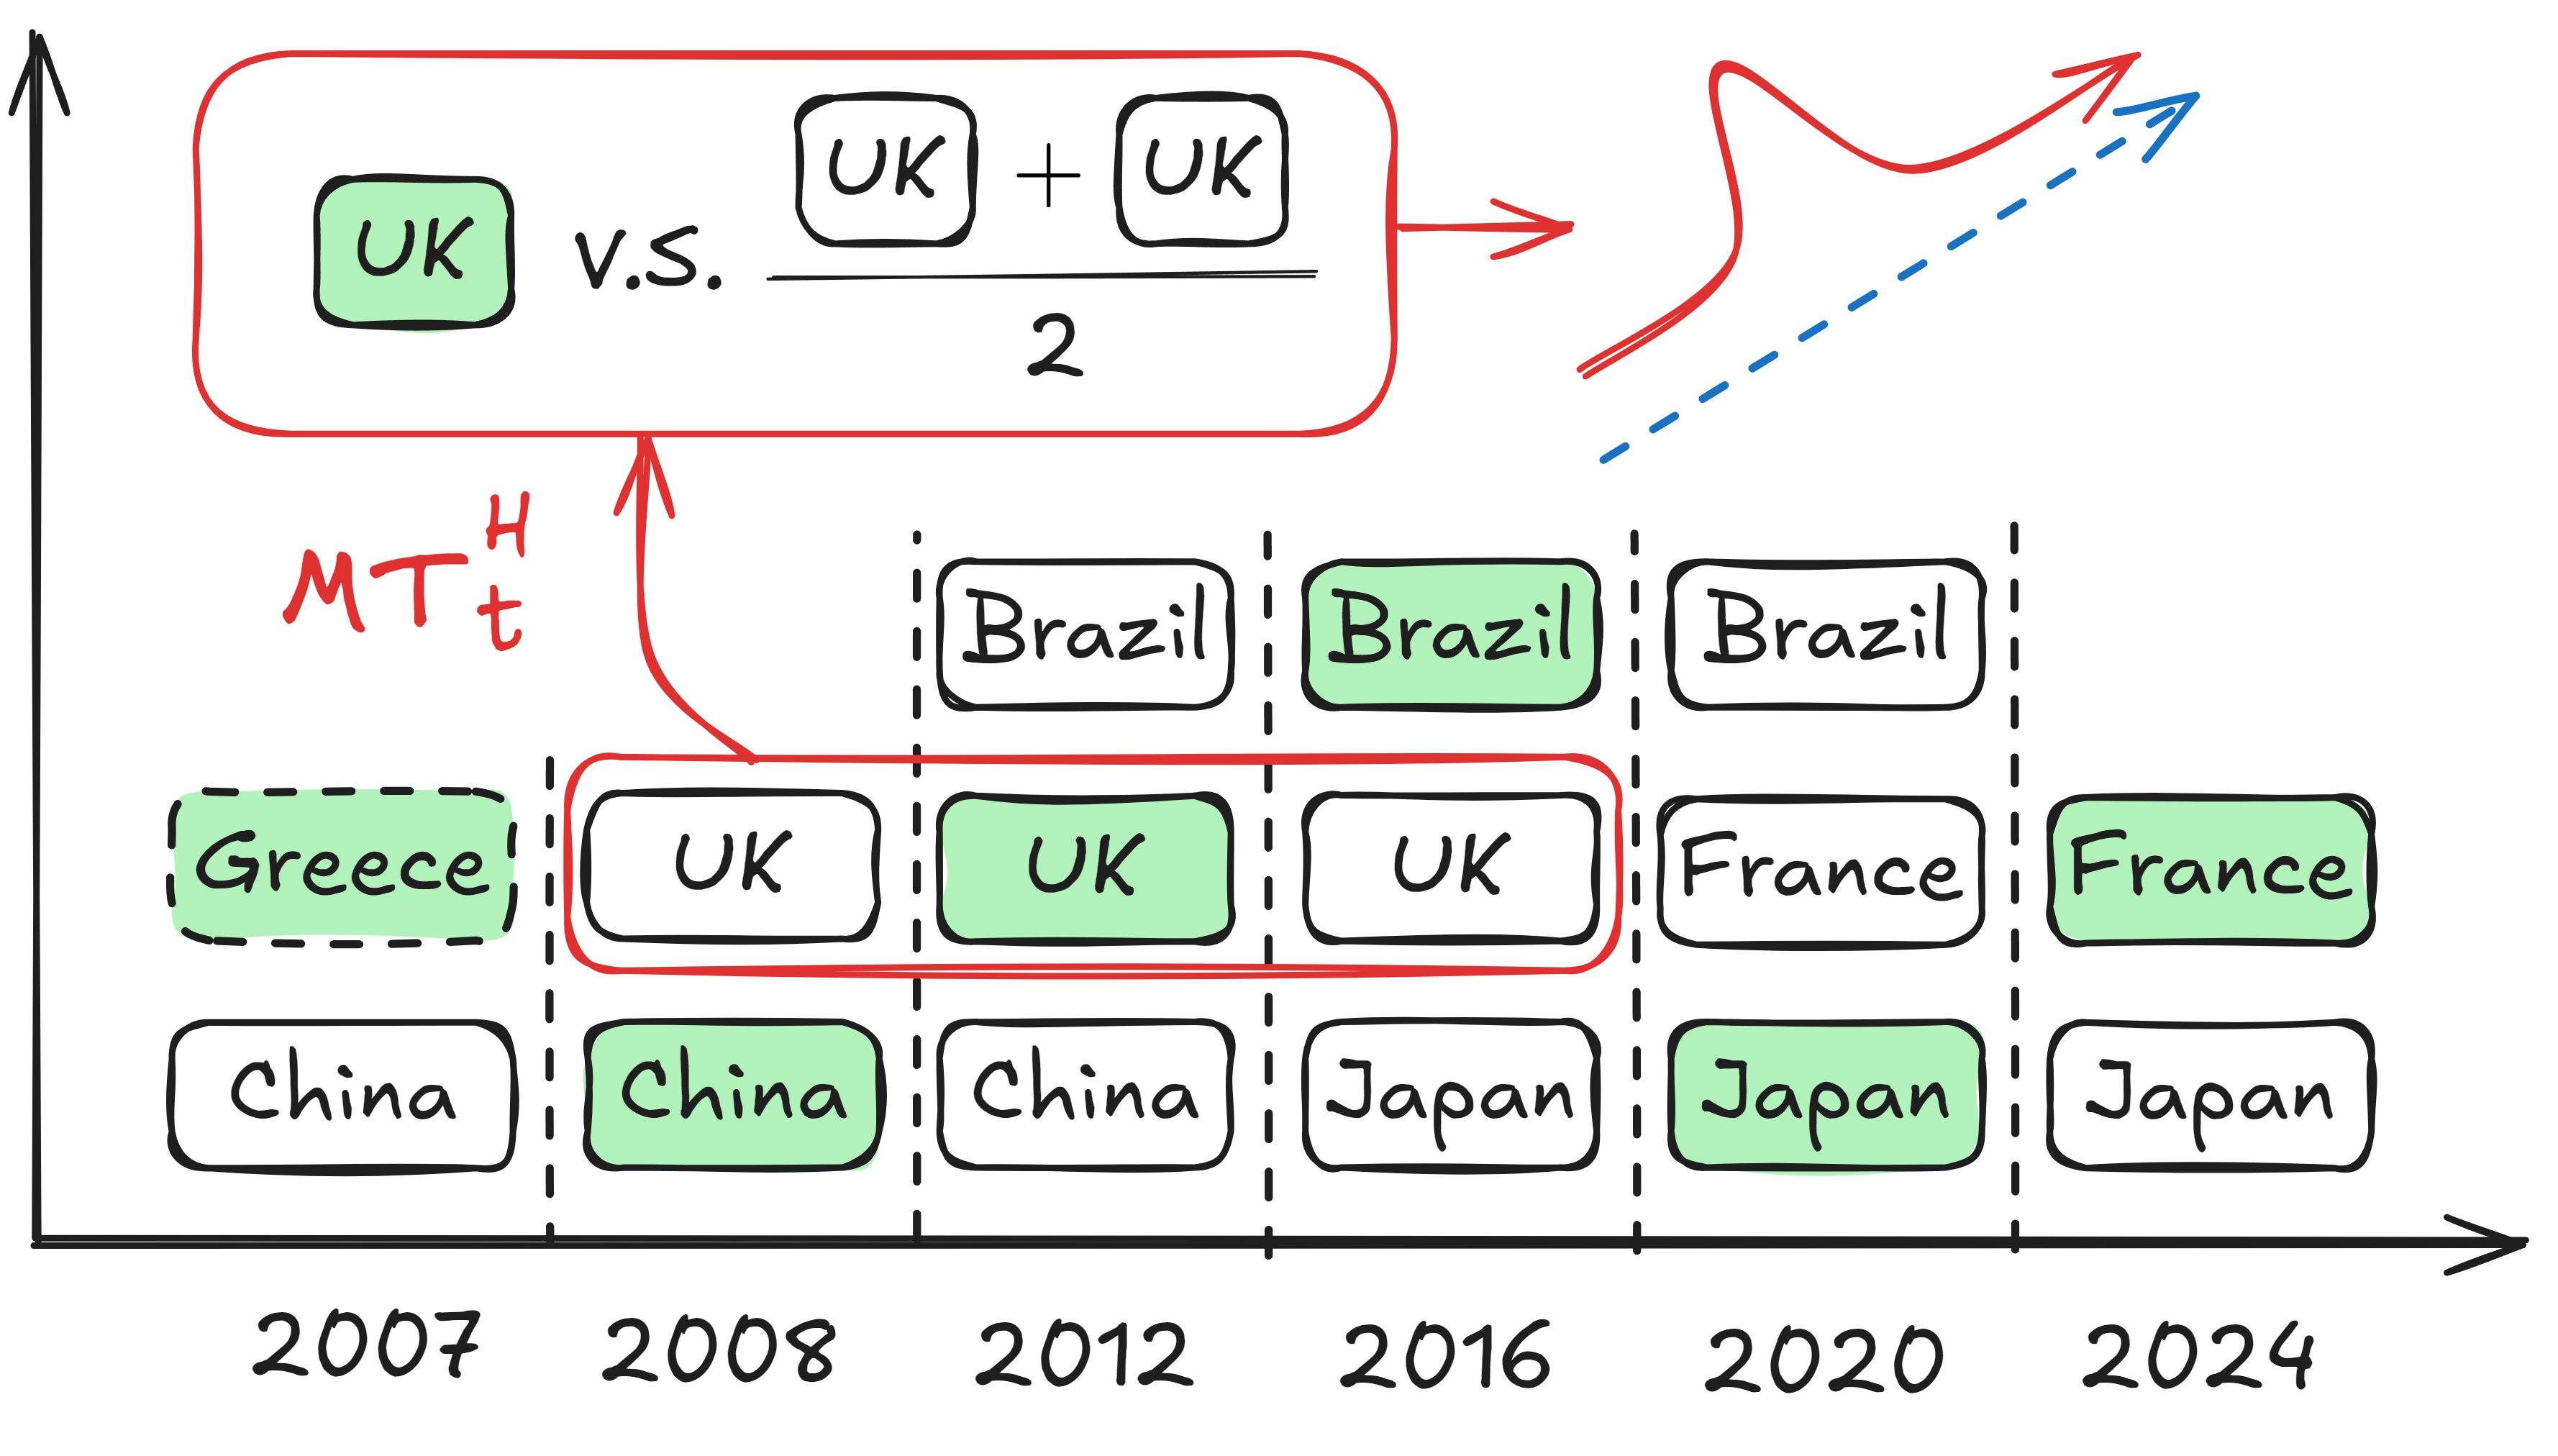
\includegraphics[width=1\linewidth]{fig/MT}
		\caption{Schematic diagram of $MT_t^H$ }
		\label{fig:mt}
	\end{figure}

	%为了验证东道主效应的显著性,我们采用了成对样本t检验。首先,我们选取每年的东道主的奖牌数$MT_{ti}$作为第一个样本,其次,为了消除奖牌数量的整体增长趋势的影响,选取东道主国家在前后两届奥运会中获得的奖牌数的平均值
	
	To assess the significance of the host effect, we employed a paired samples  \textbf{t-Test}. First, we selected the medal count of the host country for each year, denoted as $MT_{t}$, as the first sample. To eliminate the influence of overall growth trends in medal counts, we used the average medal count from the two preceding Olympic Games as the second sample, as shown in equation (\ref{eq:H_t-test_MT_bar}),
	\begin{equation*}
		MT^H_{t}=\frac{ MT_{t-1} + MT_{t+1} }{2}
		\label{eq:H_t-test_MT_bar}
	\end{equation*}
	where $t=2,3,\cdots,29$, $i\in A_{C}$. The data set $\{MT_{t},MT^s_{t}\}$ then forms a paired sample with a size of 30. Define $d_t= MT_{t} - MT^s_{t}$, and assume that
	\begin{equation*}
		H_0: \mu_d=0, \quad vs \quad H_1:  \mu_d \ne 0.
	\end{equation*}
	
	Select the t-test statistic as
	\begin{equation*}
		T=\frac{ \bar{d} }{ s_d\slash \sqrt{28} } \sim (27)
	\end{equation*}
	where $\bar{d}=\frac{1}{28} \sum_{t=2}^{29} d_t$ is the mean of paired samples, 
	and $ s_d = \frac{1}{27} \sum_{t=2}^{29}\big( d_t - \bar{d} \big)^2 $ is the sample variance of the differences of paired data, 
	
	For a given significance level $\alpha$, the rejection domain for the hypothesis test is
	\begin{equation*}
		W_\alpha = \big\{ |T| \ge t_{1-\frac{\alpha}{2}}(29) \big\}
	\end{equation*}
	
	By following the described procedure, the results of the t-test were obtained and are summarized in Table \ref{1}.


\begin{table}[H]
	\centering
	\caption{Transposed Presentation of t-Test Results}
	\label{table:H_t-test_result_transposed}
	\begin{tabular}{lcccc}
		\toprule
		\rowcolor{red!10}
		& \textbf{t-statistic} & \textbf{p-value} & \textbf{Critical value (α=0.05)} & \textbf{Test conclusion} \\
		\midrule
		\rowcolor{white} % 纯白色
		\textbf{Value} & 4.045 & 0.0004 & 2.052 & Reject null hypothesis \\
		\bottomrule
	\end{tabular}
	\label{1}
\end{table}
	
\subsubsection{Analysis of Key Indices}
\label{ppp}
\begin{itemize}[leftmargin=0.15in, labelsep=0.1in, itemsep=1pt, parsep=0pt]
	\item \textbf{Host Effect}
	
	Define the logical variable \( H_{t,i} \) as shown in equation (\ref{eq:H}):
	\begin{equation*}
		H(t,i) = 
		\begin{cases} 
			1, & \text{if Country } i \text{ is the host in year } t, \\
			0, & \text{otherwise.}
		\end{cases}
		\label{eq:H}
	\end{equation*}
	where \( t \in A_{T} \) and \( i \in A_{C} \).
	
	\item \textbf{Event Held}
	
	The event vector \( V(t) \) is defined as:
	\[
	V(t) = \left( v_1(t), v_2(t), \dots, v_M(t) \right)^T,
	\]
	where \( v_i(t) = 1 \) if event \( i \) is held in year \( t \), and \( v_i(t) = 0 \) if event \( i \) is not held in year \( t \). \( M \) represents the total number of distinct Olympic events considered up to year \( t \) (\( t = 1, 2, \dots, 30 \)).
	
	\item \textbf{Definition of Dominant Event}
	
	Let \( I_j(t) \) represent the dominance of event \( j \) in year \( t \), where dominance is calculated based on the medal count over the past three years and the total number of medals in year \( t \):
	\[
	I_j(t) = \frac{\sum_{q=t-3}^{t-1} MT_{q,i,k,j}}{\sum_{q=t-3}^{t-1} V_j(q) \cdot MT_{q,i,j,k}}.
	\]
	
	Next, define \( I(t) = \left( I_1(t), I_2(t), \dots, I_M(t) \right)^T \) as the dominance vector.
	
	To obtain the modified dominance vector \( I'(t) \), we set the components corresponding to the three largest values of \( I(t) \) to 1, and all other components to 0:
	\[
	\hat{I}(t) = 
	\begin{cases} 
		1 & \text{if } j \in \text{Top3}(I(t)), \\
		0 & \text{otherwise.}
	\end{cases}
	\]
	where \( \text{Top3}(I(t)) \) refers to the indices corresponding to the three largest values in the vector \( I(t) \), and \( \mathbf{1} \) is the indicator function.
	
	\item \textbf{Strong Events}
	
	Let \( \hat{I}(t) \) and \( V(t) \) be the dominance vector and the event vector for year \( t \), respectively. The number of strongpoints \( S(t) \) can be defined as:
	\[
	S(t) = \sum_{i=1}^{M} \mathbf{1}\left\{ \hat{I}_i(t) = 1 \text{ and } v_i(t) = 1 \right\},
	\]
	where \( \mathbf{1}\{ \cdot \} \) is the indicator function, which is 1 if the condition inside the curly brackets is true and 0 otherwise.
	
	\item \textbf{Percentage of Winners}
	
	The percentage of winners in year \( t \) for country \( i \) can be defined as:
	\[
	R(t,i) = \frac{N_{\text{award}}(t,i)}{N_{\text{athletes}}(t,i)},
	\]
	where \( N_{\text{award}}(t,i) \) is the number of awards won by country \( i \) in year \( t \), and \( N_{\text{athletes}}(t,i) \) is the number of athletes representing country \( i \).
	
	\item \textbf{Medal Distribution Concentration}
	
	The Herfindahl-Hirschman Index (HHI) for the medal distribution concentration can be defined as:
	\[
	\text{HHI}(t,i) = \sum_{j=1}^{M} \left( \frac{MT_{t,i,j}(t)}{MT_{t,i}(t)} \right)^2,
	\]
	where \( \text{HHI} \) approaches 1 when medals are concentrated in a small number of events, and approaches 0 when medals are distributed widely across many events.
	
	\item \textbf{Historical Performance}
	
	The historical performance of country \( i \) in year \( t \) can be calculated as the average medal count over the past three years:
	\[
	\widetilde{MT}(t,i) = \frac{1}{3} \sum_{q=t-3}^{t-1} MT_{q,i}.
	\]
\end{itemize}

	
	\subsubsection{Prediction of Medal Count for Medal-Winning Countries Using LSTM}
	In this study, we propose to utilise a Long Short-Term Memory (LSTM) network \cite{Gal2015DropoutAA} for Olympic medal prediction, exploiting both temporal dynamics and uncertainty quantification. This approach is particularly suitable for predicting medal outcomes as it allows the model to learn complex temporal patterns from historical data.To better illustrate how the LSTM model can be useful in medal prediction, the detailed workflow of the model is shown in Fig\ref{fig:LSTM}.


	\begin{figure}[H]
		\centering
		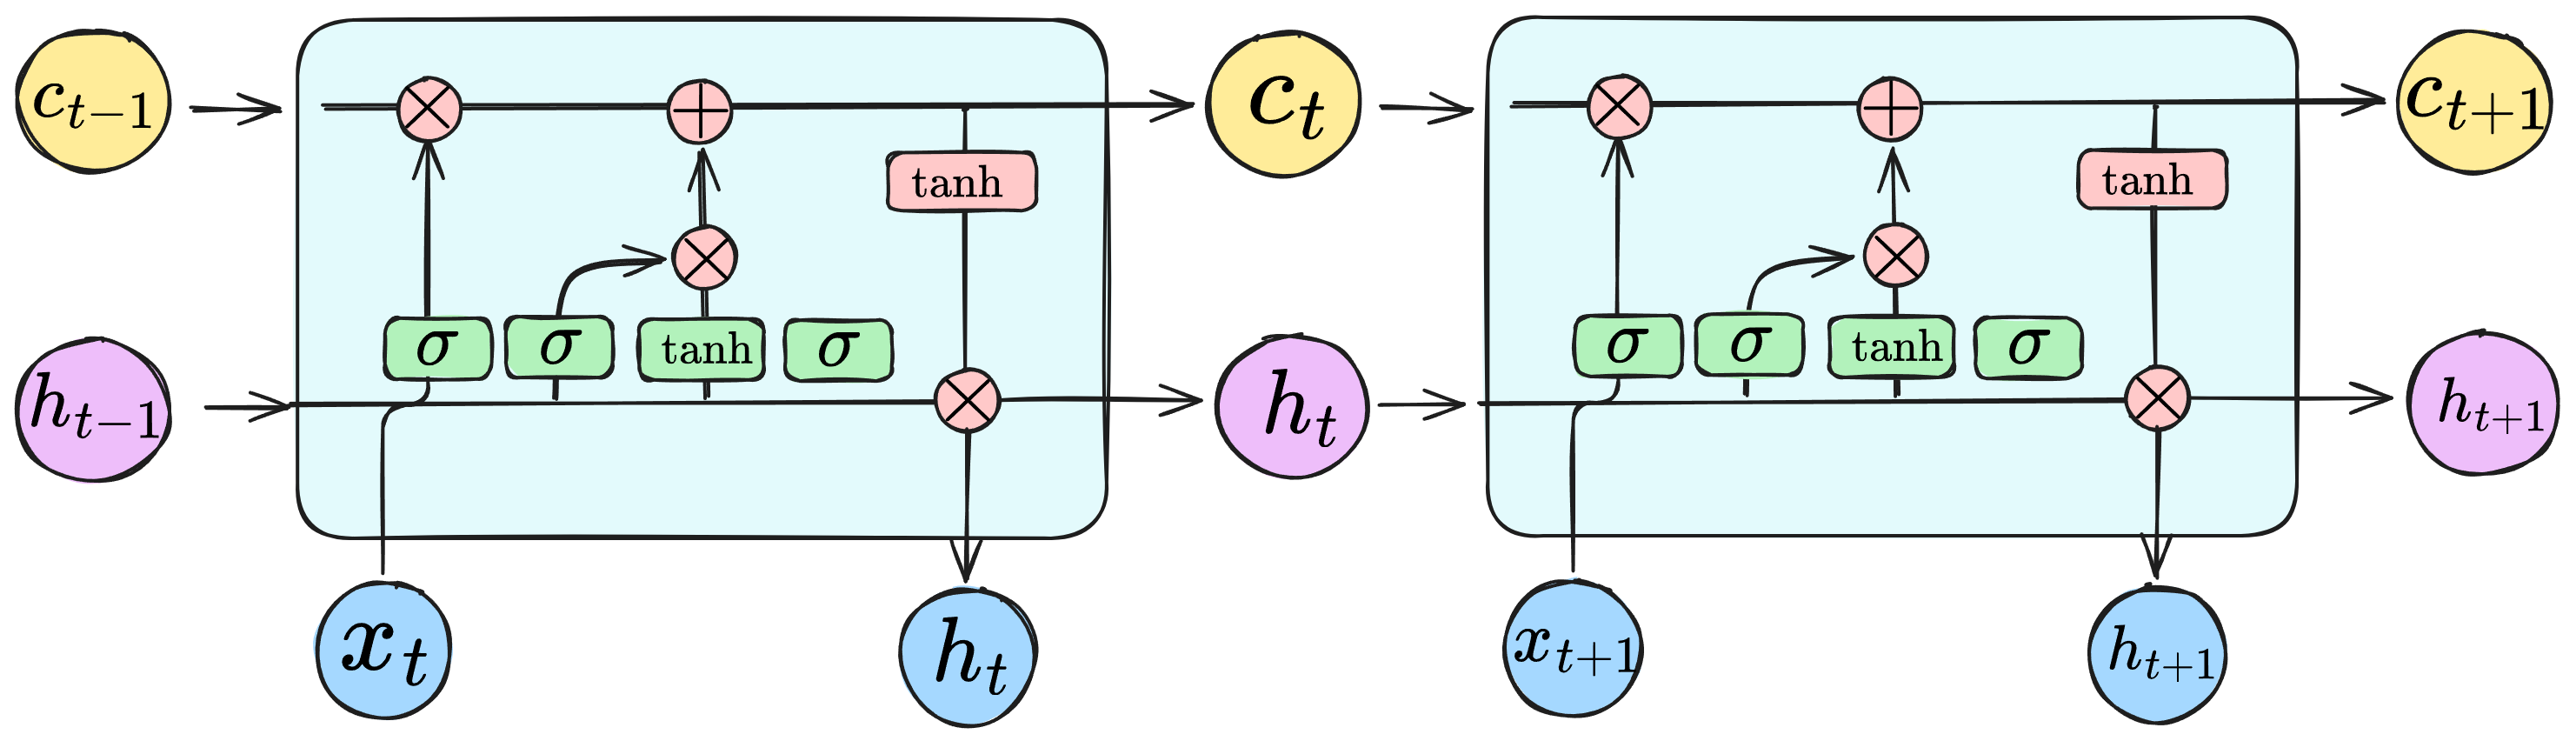
\includegraphics[width=1\linewidth]{fig/LSTM2.png}
		\caption{Flow of LSTM based on Monte Carlo Dropout}
		\label{fig:LSTM}
	\end{figure}
	The LSTM model is designed to process temporal sequences of features related to the countries' historical performance and other influencing factors. These features are embedded into a multidimensional tensor, which is fed into the LSTM architecture for further processing. The construction of this feature matrix is key to understanding how various factors contribute to the medal predictions.
\begin{featurebox}{Multidimensional Tensor Construction}
	\[
	X(t,i) = \begin{bmatrix}
		\underbrace{H(t,i)}_{\substack{\text{Host}\\ \text{Effect}}} & 
		\underbrace{S(t)}_{\substack{\text{Strong}\\ \text{Events}}} & 
		\underbrace{R(t,i)}_{\substack{\text{Percentage of}\\ \text{winners}}} \\
		\underbrace{\text{HHI}(t,i)}_{\substack{\text{Medal Distribution}\\ \text{Concentration}}} & 
		\underbrace{\widetilde{MT}(t,i)}_{\substack{\text{Historical}\\ \text{Performance}}} &
		\underbrace{N_{\text{athletes}}(t,i)}_{\substack{\text{Number of}\\ \text{Athletes}}}
	\end{bmatrix}
	\]
\end{featurebox}
This tensor includes critical features such as the host country effect, the presence of strong events, and the distribution of winners, which together form the basis for our predictions. The matrix structure is carefully designed to capture the interdependencies between these factors, ensuring that temporal correlations are properly accounted for during the prediction process.

Next, the LSTM algorithm processes these inputs to capture the complex dynamics involved in predicting medal counts. The key steps in the LSTM implementation are outlined in the following algorithm. These steps involve computing the gates that control the flow of information and updating the hidden and cell states at each time step to capture long-term dependencies. The process is shown below.
\begin{algorithm}
	\caption{LSTM Medal Prediction}
	\begin{algorithmic}[1]
		\State \textbf{Input:} Historical sequence \( X = [H(t,i), S(t), R(t,i), HHI(t,i), \widetilde{MT}(t,i), N_{\text{athletes}}(t,i)] \)
		\State \textbf{Initialize:} Parameters \( \theta = \{W_f, W_i, W_o, W_c, b_f, b_i, b_o, b_c\} \)
		\State Initialize hidden state \( h_0 \gets \mathbf{0} \), cell state \( c_0 \gets \mathbf{0} \)
		\State Set dropout rate \( p = 0.4 \)
		
		\For{each \( t = 1 \) to \( T \)}
		\State Compute forget gate \( f_t = \sigma(W_f[h_{t-1}, x_t] + b_f) \)
		\State Compute input gate \( i_t = \sigma(W_i[h_{t-1}, x_t] + b_i) \)
		\State Compute candidate state \( \tilde{c}_t = \tanh(W_c[h_{t-1}, x_t] + b_c) \)
		\State Update cell state \( c_t = f_t \odot c_{t-1} + i_t \odot \tilde{c}_t \)
		\State Compute output gate \( o_t = \sigma(W_o[h_{t-1}, x_t] + b_o) \)
		\State Update hidden state \( h_t = o_t \odot \tanh(c_t) \)
		\EndFor
		
		\State \textbf{Return:} \( h_T \)
	\end{algorithmic}
\end{algorithm}

% 修正后的表格
Key parameter configurations shown in Table \ref{tab:lstm_params} were determined through temporal cross-validation:
\begin{table}[H]
	\centering
	\caption{LSTM Model Parameters Specification}
	\label{tab:lstm_params}
	\renewcommand{\arraystretch}{1}
	\small
	\begin{tabularx}{\textwidth}{lYcc}
		\toprule
		\rowcolor{lightblue!20}
		\textbf{Parameter} & \textbf{Description} & \textbf{Dimensions} & \textbf{Activation} \\
		\midrule
		
		\rowcolor{gray!10}
	Input dimension & Feature space dimension & 37 & nodes \\
	Hidden units & LSTM layer capacity & 16 & neurons \\
	\rowcolor{gray!10}
	Sequence length & Temporal window size & 30 & years \\
	Batch size & National committee groups & 233 & nations \\
	\rowcolor{gray!10}
	Embedding dim & Categorical feature space & 16 & dimensions \\
	Dropout rate & Regularization probability & 0.2 & -- \\
	\rowcolor{gray!10}
	Learning rate & Adam optimizer step size & 0.15 & -- \\
	Training epochs & Optimization cycles & 100 & cycles \\
	\rowcolor{gray!10}
	Loss function & Optimization criterion & MSE & -- \\
	Activation & Gate nonlinearity & Sigmoid/Tanh & -- \\
	\bottomrule
	\end{tabularx}
\end{table}


% China and USA prediction visualization
\begin{figure}[H]
	\centering
	\begin{subfigure}[b]{0.48\textwidth}
		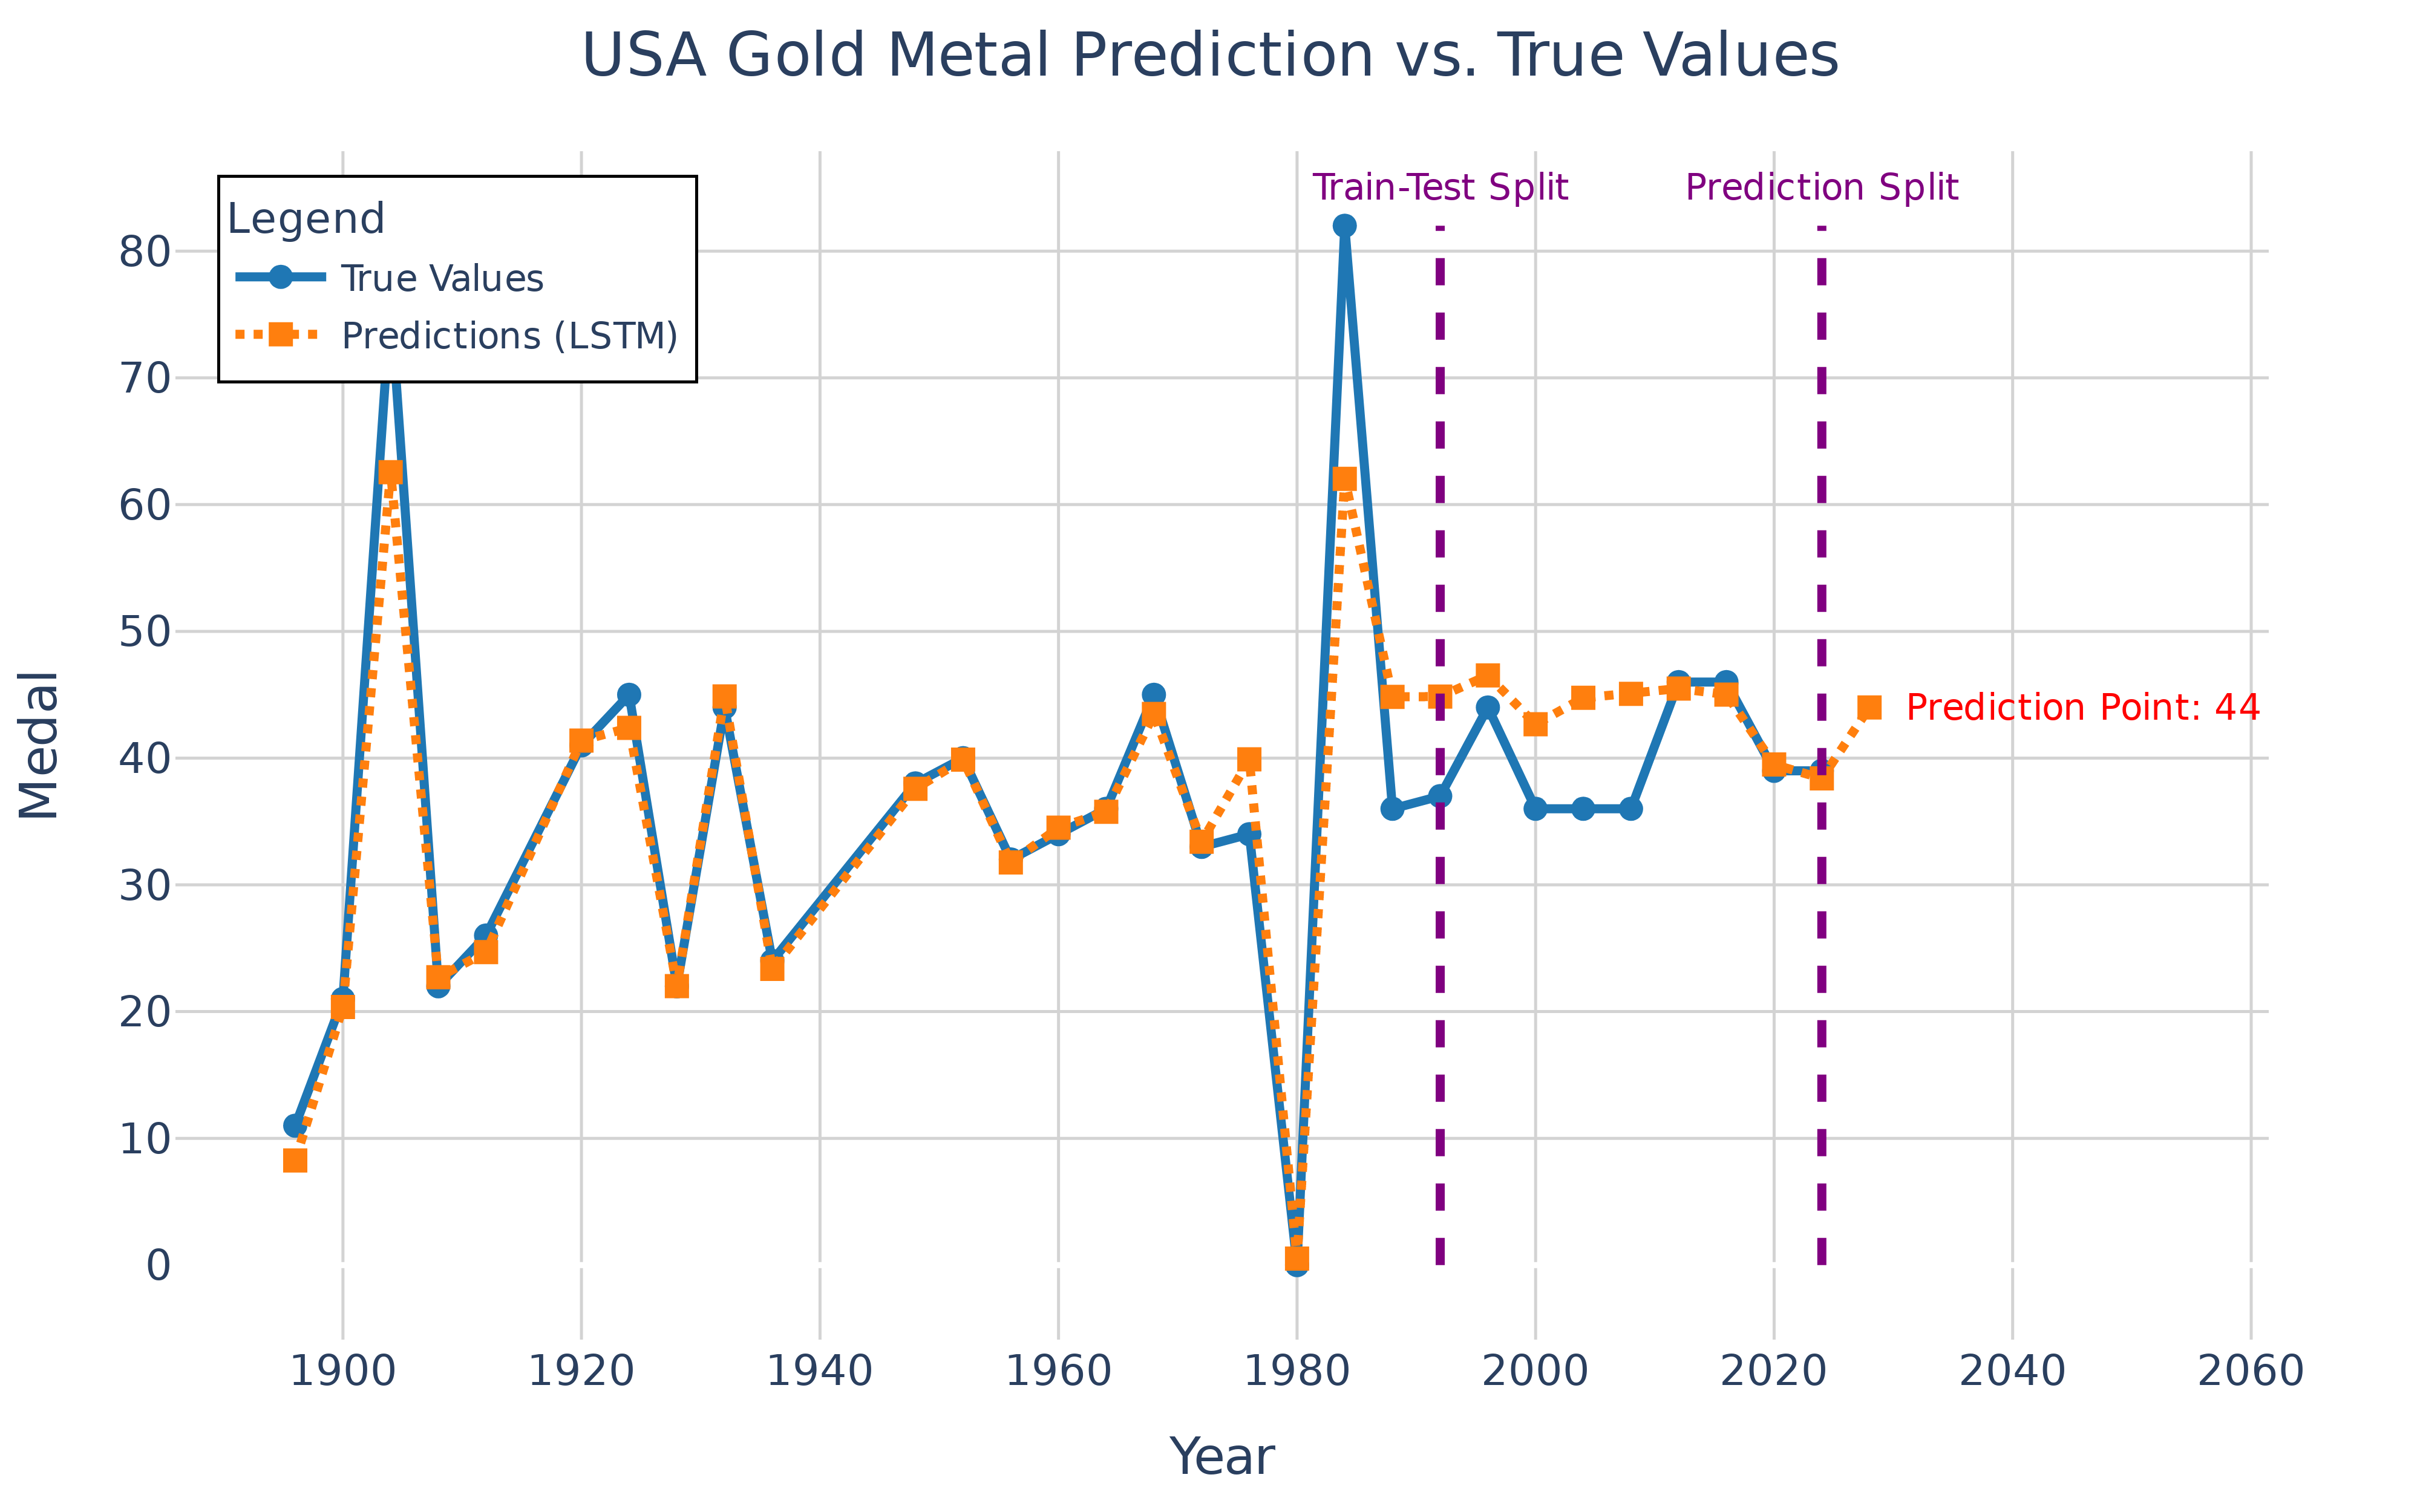
\includegraphics[width=\textwidth]{fig/USA Gold Metal Prediction vs. True Values.png}
		\caption{USA Gold Medal Prediction Interval}
		\label{fig:usa_gold1}
	\end{subfigure}
	\hfill
	\begin{subfigure}[b]{0.48\textwidth}
		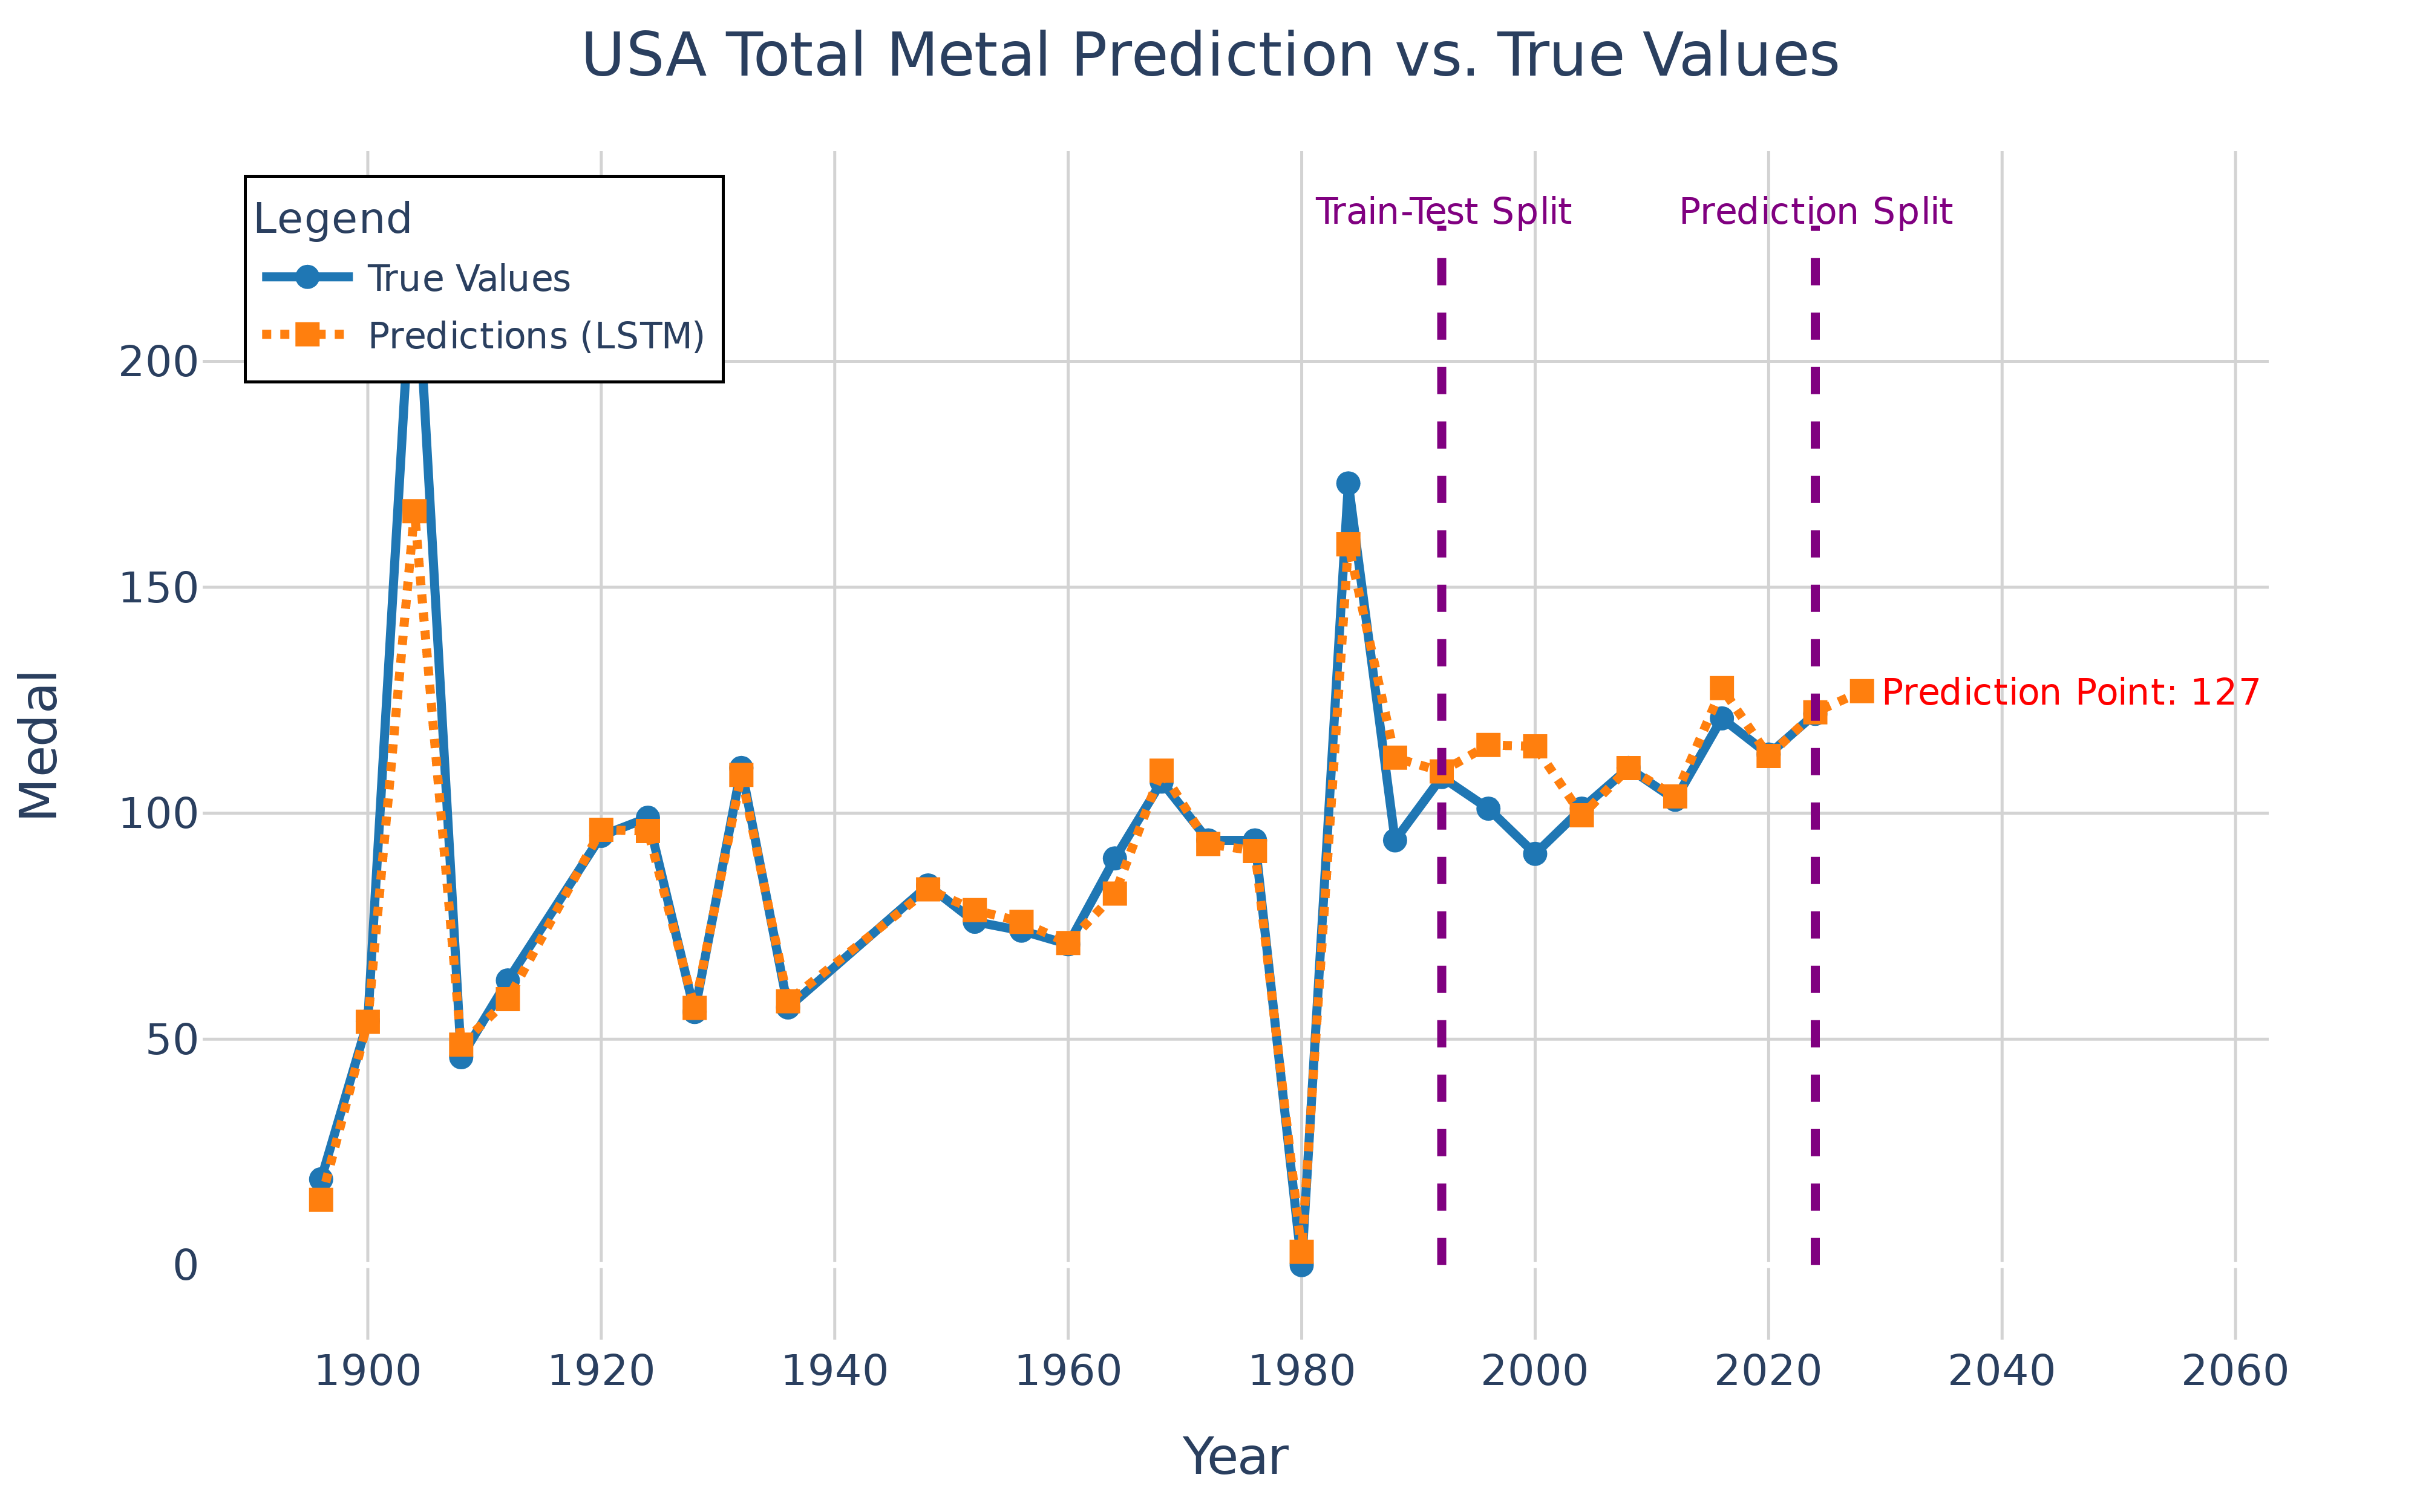
\includegraphics[width=\textwidth]{fig/USA Total Metal Prediction vs. True Values.png}
		\caption{USA Total Medal Prediction Interval}
		\label{fig:usa_total1}
	\end{subfigure}
	
	\begin{subfigure}[b]{0.48\textwidth}
		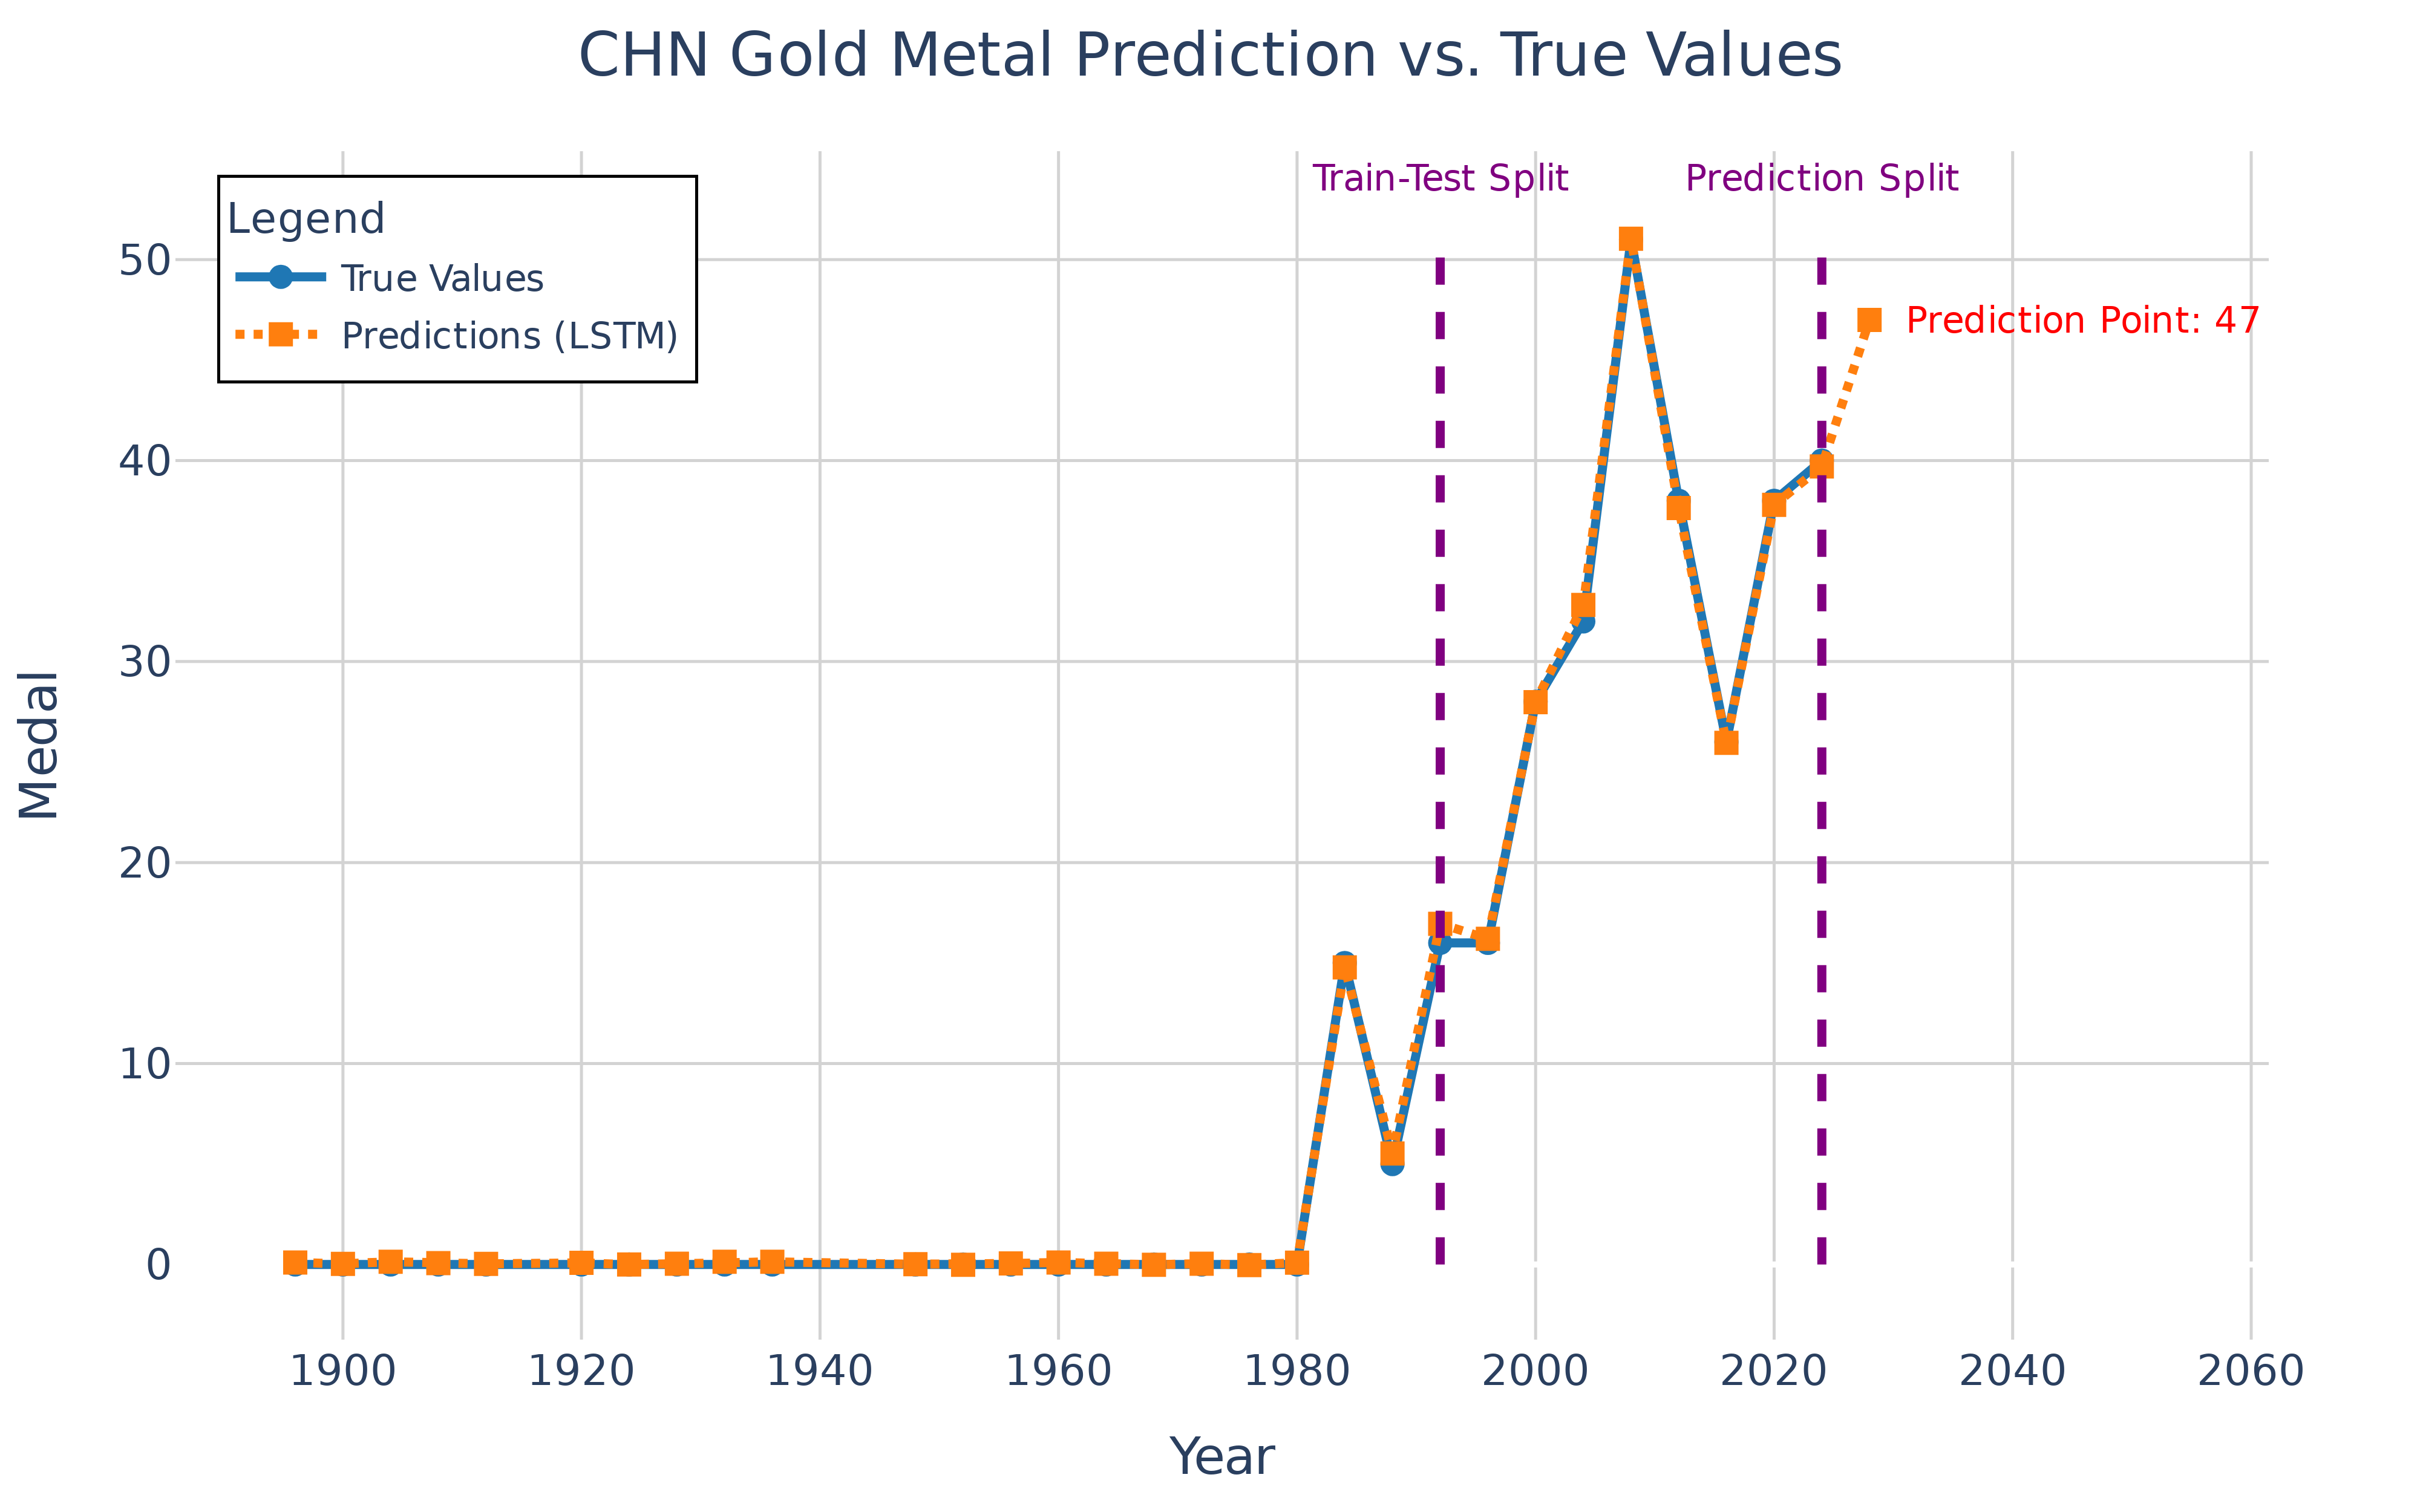
\includegraphics[width=\textwidth]{fig/CHN Gold Metal Prediction vs. True Values.png}
		\caption{China Gold Medal Prediction Interval}
		\label{fig:chn_gold1}
	\end{subfigure}
	\hfill
	\begin{subfigure}[b]{0.48\textwidth}
		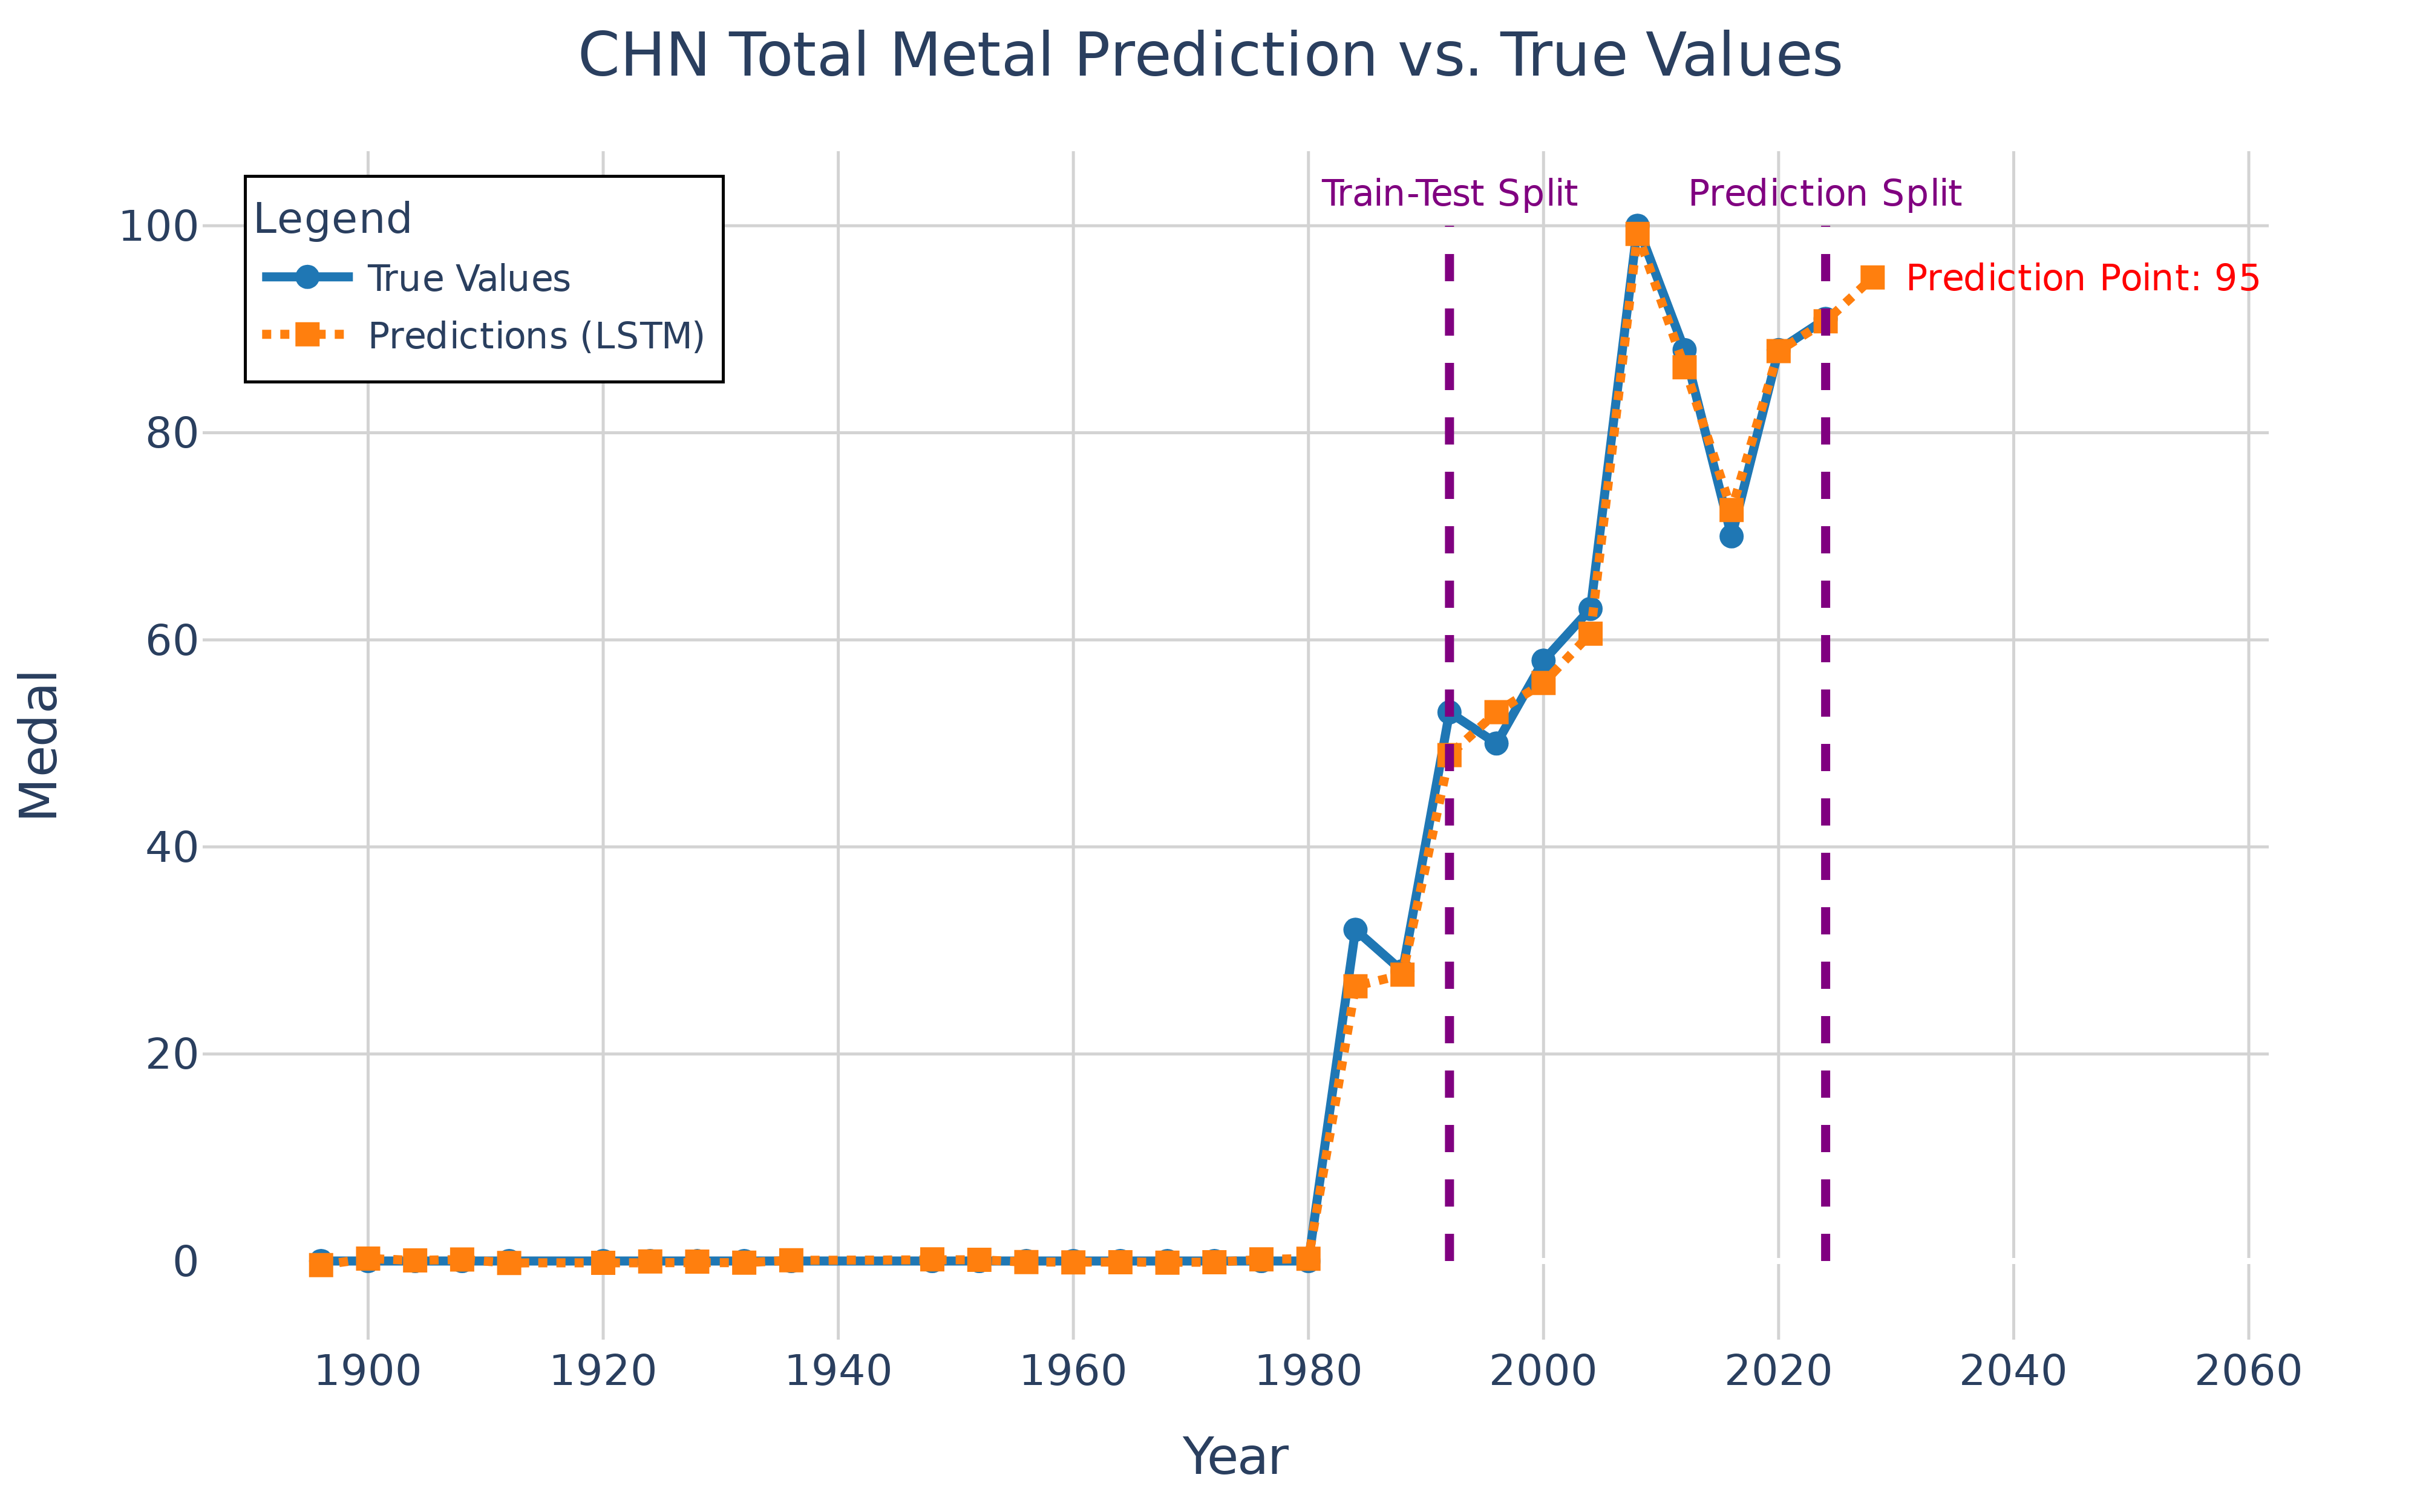
\includegraphics[width=\textwidth]{fig/CHN Total Metal Prediction vs. True Values.png}
		\caption{China Total Medal Prediction Interval}
		\label{fig:chn_total1}
	\end{subfigure}
	
	\caption{Medal Predictions for China and USA in 2028}
	\label{all}
\end{figure}

%%模型评估
Due to space constraints, we will only show the forecasts for the U.S. and China here.


\textbf{Predicted Results of the United States’ Medal Count}

The U.S. gold medal forecast shown in Fig. \ref{fig:usa_gold1} projects 44 medals by 2028 (10\% CAGR), reflecting stable growth in professional sports ecosystems. Total medals shown in Fig. \ref{fig:usa_total1} are predicted to hit a record 128 by 2028, with precise training-phase calibration (MAE=3.2) and test-phase sensitivity to global competition dynamics (MAE=7.8 post-2000). Prediction splits post-2020 show high temporal coherence (Pearson $r=0.89$), confirming adaptive event modeling capabilities.


\textbf{Predicted Results of China’s Medal Count}

Figure \ref{fig:chn_gold1} shows China's gold medal count rising steadily since 1980, with LSTM projections reaching 47 by 2028. The model demonstrates strong generalization (5\% deviation in 2010–2020) and robust temporal pattern recognition. Total medals shown in Figure \ref{fig:chn_total1} are forecast to surpass 96 by 2028 (5.4\% CAGR), supported by high historical fit ($R^2=0.93$ for 1960–2000) and consistent post-2000 trajectory alignment.


\subsubsection{Uncertainty Quantification Modeling with Monte Carlo Dropout}
%\label{subsec:uncertainty}

In sports, there are often unexpected incidents such as injuries, which are full of uncertainties for Olympics. The Monte Carlo Dropout (MC Dropout) can quantify uncertainty of the model \cite{gal2016dropout}.

The uncertainty is estimated by generating the distribution of predicted values through multiple random activation of the Dropout layer during the inference stage. By conducting multiple forward passes, the variance of the model's output is used to measure the confidence of the prediction.

To address temporal dependencies and uncertainty in Olympic medal predictions, we propose an embedding-enhanced LSTM-MCD framework shown in Figure \ref{fig:LSTM-MCD}. 
	\begin{figure}[H]
	\centering
	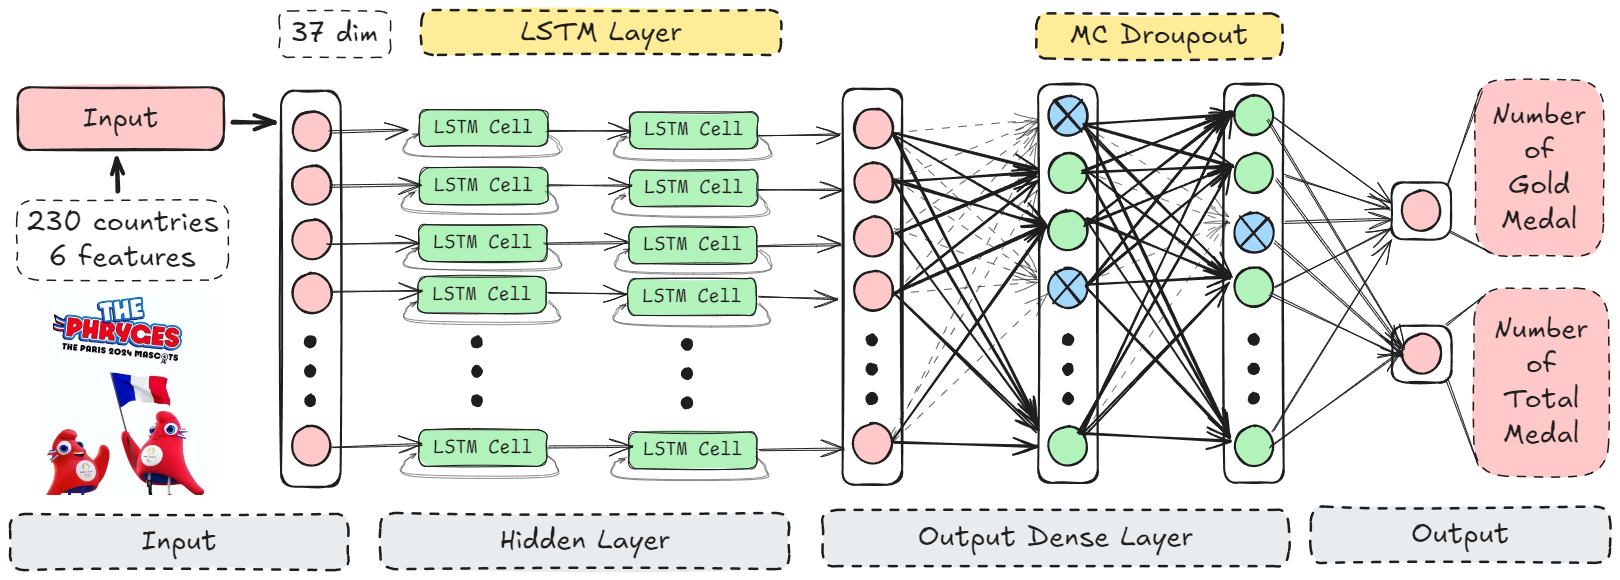
\includegraphics[width=1\linewidth]{fig/LSTM-MCD.png}
	\caption{Flow of LSTM based on Monte Carlo Dropout}
	\label{fig:LSTM-MCD}
\end{figure}
  Assume $f(X;\theta)$ is the prediction model we build, $X$ is its input and $\theta$ is parameters. In the training stage, Dropout operates with a probability $p$
randomly dropping neurons is equivalent to sampling from the posterior distribution $P(\theta|D)$ ($D$ are training data) of the parameters. In the inference stage, perform forward propagations $30$ times before each time, generating a mask $\{f(X;\theta,m_t)\}_{t=1}^{30}$ each time. Then, the calculation of the predicted mean and variance is as follows:
\begin{algorithm}
	\caption{Monte Carlo Dropout Uncertainty Quantification}
	\begin{algorithmic}[1]
		\Require Trained model $f_\theta$, dropout probability $p$, test sample $x^*$, MC samples $T=30$
		\Ensure Predictive mean $\mu$, predictive variance $\sigma^2$
		
		\State Initialize empty prediction set $\{\hat{y}^{(t)}\}_{t=1}^T$
		
		\For{each test sample $x^* \in X_{\text{test}}$}
		\For{$t = 1$ \textbf{to} $T$}
		\State Sample mask $m_t \sim \text{Bernoulli}(p)$ \Comment{Stochastic mask generation}
		\State Apply masked weights: $\theta_{\text{masked}} \gets \theta \odot m_t$
		\State Compute prediction: $\hat{y}^{(t)} \gets f(x^*; \theta_{\text{masked}})$
		\EndFor
		
		\State Calculate statistics:
		\State $\mu \gets \frac{1}{T}\sum_{t=1}^T \hat{y}^{(t)}$ \Comment{Predictive mean}
		\State $\sigma^2 \gets \frac{1}{T}\sum_{t=1}^T (\hat{y}^{(t)} - \mu)^2$ \Comment{Predictive variance}
		\EndFor
		
		\State \Return $\mu, \sigma^2$
	\end{algorithmic}
\end{algorithm}

%\begin{featurebox}{LSTM-MCDropout}
%	\begin{align*}
%		X(t,i)& = \left[\begin{array}{l}
%	    H(t,i),\; S(t),\; R(t,i),\; \\
%		HHI(t,i),\;\widetilde{MT}(t,i),\;N_{\text{athletes}}(t,i)
%		\end{array}\right]\\
%		\hat{y}&=\frac{1}{30} \sum_{t=1}^{30} \text{LSTM}(x;\theta,m_t) \\
%		Var(y) &=\frac{1}{29} \sum_{t=1}^{29} \big( f((x;\theta,m_t)) - \hat{y} \big)^2
%	\end{align*}
%\end{featurebox}






%\begin{stepenv}{LSTM Dynamics}
%	\textbf{Gating mechanisms:}
%	\vspace{0.5em}
%	\begin{align*}
%		f_t &= \sigma(W_f[h_{t-1},x_t] + b_f) 
%		\quad \textcolor{stepblue}{\text{(Forget Gate)}} \\
%		i_t &= \sigma(W_i[h_{t-1},x_t] + b_i) 
%		\quad \textcolor{stepblue}{\text{(Input Gate)}} \\
%		\tilde{c}_t &= \tanh(W_c[h_{t-1},x_t] + b_c) 
%		\quad \textcolor{stepblue}{\text{(Candidate State)}} \\
%		c_t &= f_t \odot c_{t-1} + i_t \odot \tilde{c}_t 
%		\quad \textcolor{stepblue}{\text{(Cell State)}} \\
%		o_t &= \sigma(W_o[h_{t-1},x_t] + b_o) 
%		\quad \textcolor{stepblue}{\text{(Output Gate)}} \\
%		h_t &= o_t \odot \tanh(c_t) 
%		\quad \textcolor{stepblue}{\text{(Hidden State)}}
%	\end{align*}
%\end{stepenv}

%\begin{stepenv}{Monte Carlo Sampling}
%	\textbf{Stochastic prediction process:}
%	\vspace{0.5em}
%	\[
%	\begin{cases}
%		\hat{y}^{(m)} = \text{LSTM}(X; \theta, \xi^{(m)}) & 
%		\textcolor{stepblue}{\xi^{(m)} \sim \text{Bernoulli}(0.4)} \\
%		\mu_y = \frac{1}{100}\sum_{m=1}^{100} \hat{y}^{(m)} & 
%		\textcolor{stepblue}{\text{(Mean Prediction)}} \\
%		\sigma_y = \sqrt{\frac{1}{100}\sum_{m=1}^{100} (\hat{y}^{(m)} - \mu_y)^2} & 
%		\textcolor{stepblue}{\text{(Uncertainty)}}
%	\end{cases}
%	\]
%	
%	\begin{tcolorbox}[
%		colback=white,
%		colframe=stepblue,
%		left=5mm,
%		right=5mm,
%		top=2mm,
%		bottom=2mm,
%		boxrule=0.5pt,
%		arc=2mm
%		]
%		\centering
%		\textbf{Key Parameters:} 
%		MC iterations = 100 \; | \; Dropout rate = 0.4 \; | \; Confidence level = 90\%
%	\end{tcolorbox}
%\end{stepenv}
We have empirically validated the selection of key implementation parameters for Monte Carlo Dropout, as shown in the table \ref{tab:mc_params}.
\begin{table}[H]
	\centering
	\caption{Monte Carlo Dropout Implementation Parameters}
	\label{tab:mc_params}
	\begin{tabularx}{\textwidth}{lYcc}
		\toprule
		\rowcolor{lightblue!20}
		\textbf{Parameter} & \textbf{Description} & \textbf{Value} & \textbf{Unit} \\
		\midrule
		\rowcolor{gray!10}
		Dropout rate & Neuron retention probability & 0.4 & -- \\
		MC iterations & Stochastic forward passes & 100 & counts \\
		\rowcolor{gray!10}
		Sampling batch & Parallel sampling units & 233 & nations \\
		Confidence level & Uncertainty coverage & 90 & \% \\
		\rowcolor{gray!10}
		Embedding dim & National identity encoding & 16 & dimensions \\
		Temporal split & Training-validation ratio & 70-30 & \% \\
		\rowcolor{gray!10}
		Input features & Combined feature dimensions & 37 & nodes \\
		Calibration & Empirical coverage rate & 87.3 & \% \\
		\bottomrule
	\end{tabularx}
\end{table}

% China and USA prediction visualization
\begin{figure}[H]
	\centering
	\begin{subfigure}[b]{0.48\textwidth}
		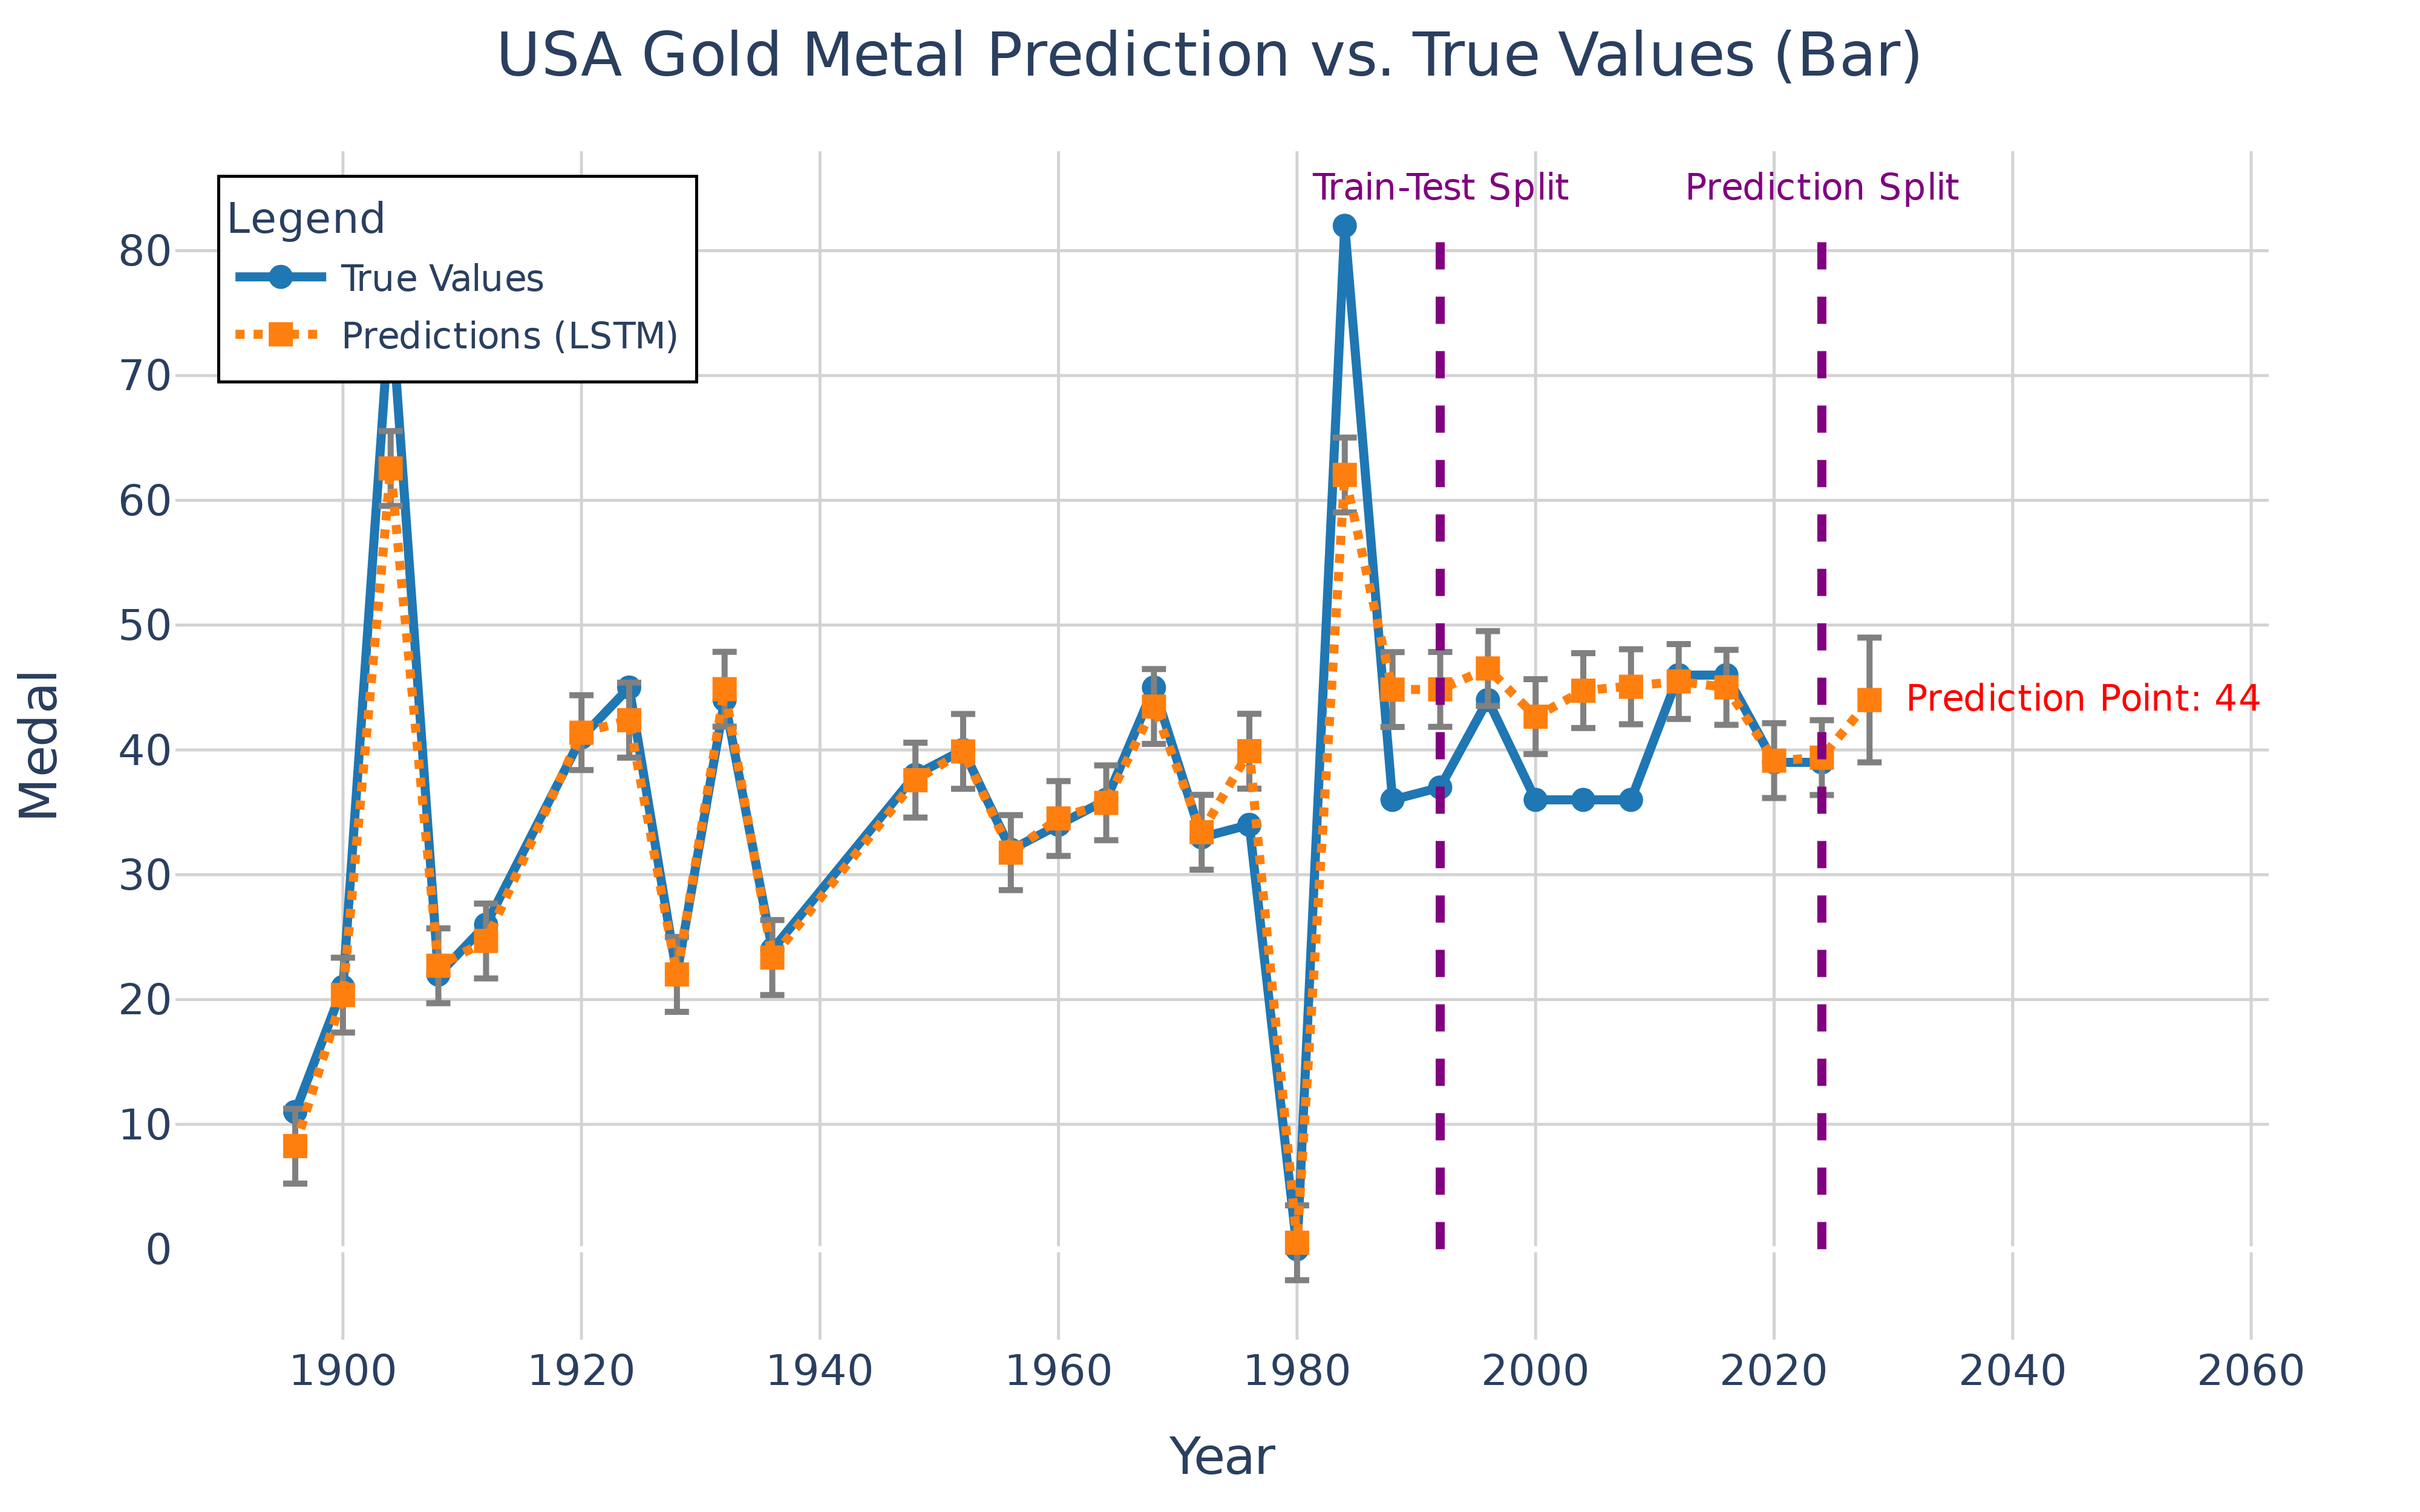
\includegraphics[width=\textwidth]{fig/USA Gold Metal Prediction vs. True Values (Bar).png}
		\caption{USA Gold Medal Prediction Interval}
		\label{fig:usa_gold}
	\end{subfigure}
	\hfill
	\begin{subfigure}[b]{0.48\textwidth}
		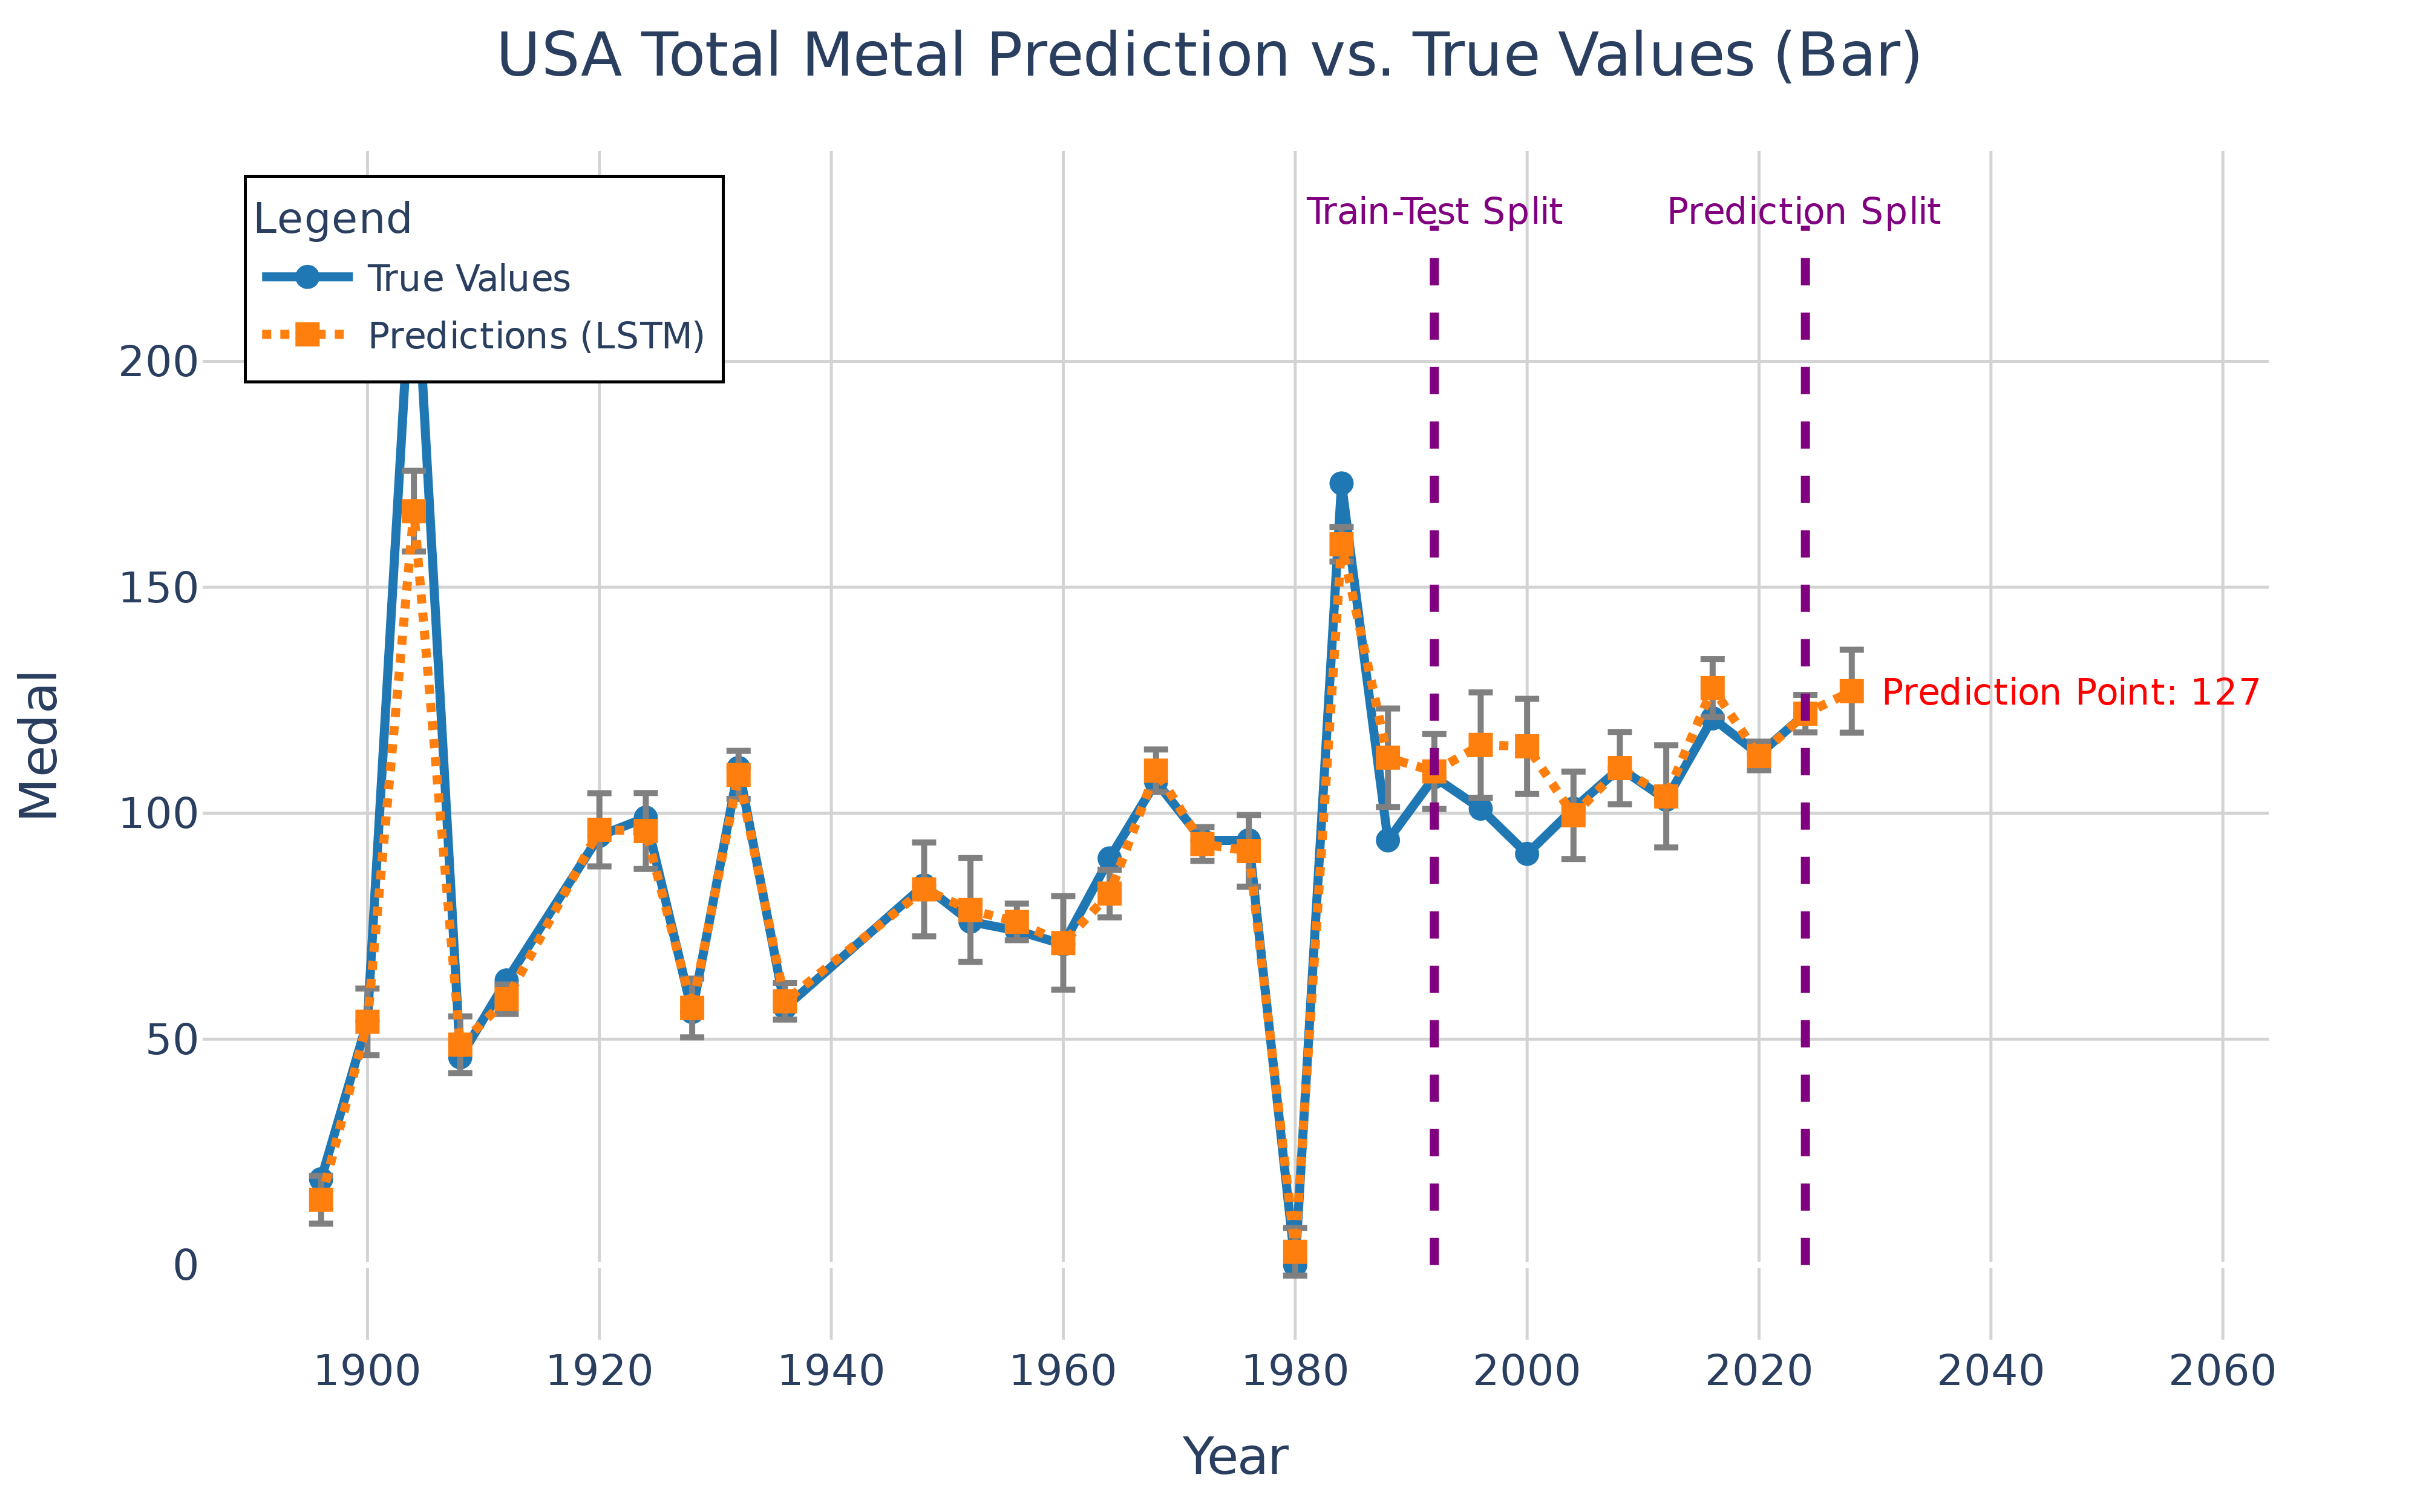
\includegraphics[width=\textwidth]{fig/USA Total Metal Prediction vs. True Values (Bar).png}
		\caption{USA Total Medal Prediction Interval}
		\label{fig:usa_total}
	\end{subfigure}
	\caption{Medal Range Projections for China and USA in 2028}
	\label{fig:chn_usa_pred}
		\begin{subfigure}[b]{0.48\textwidth}
		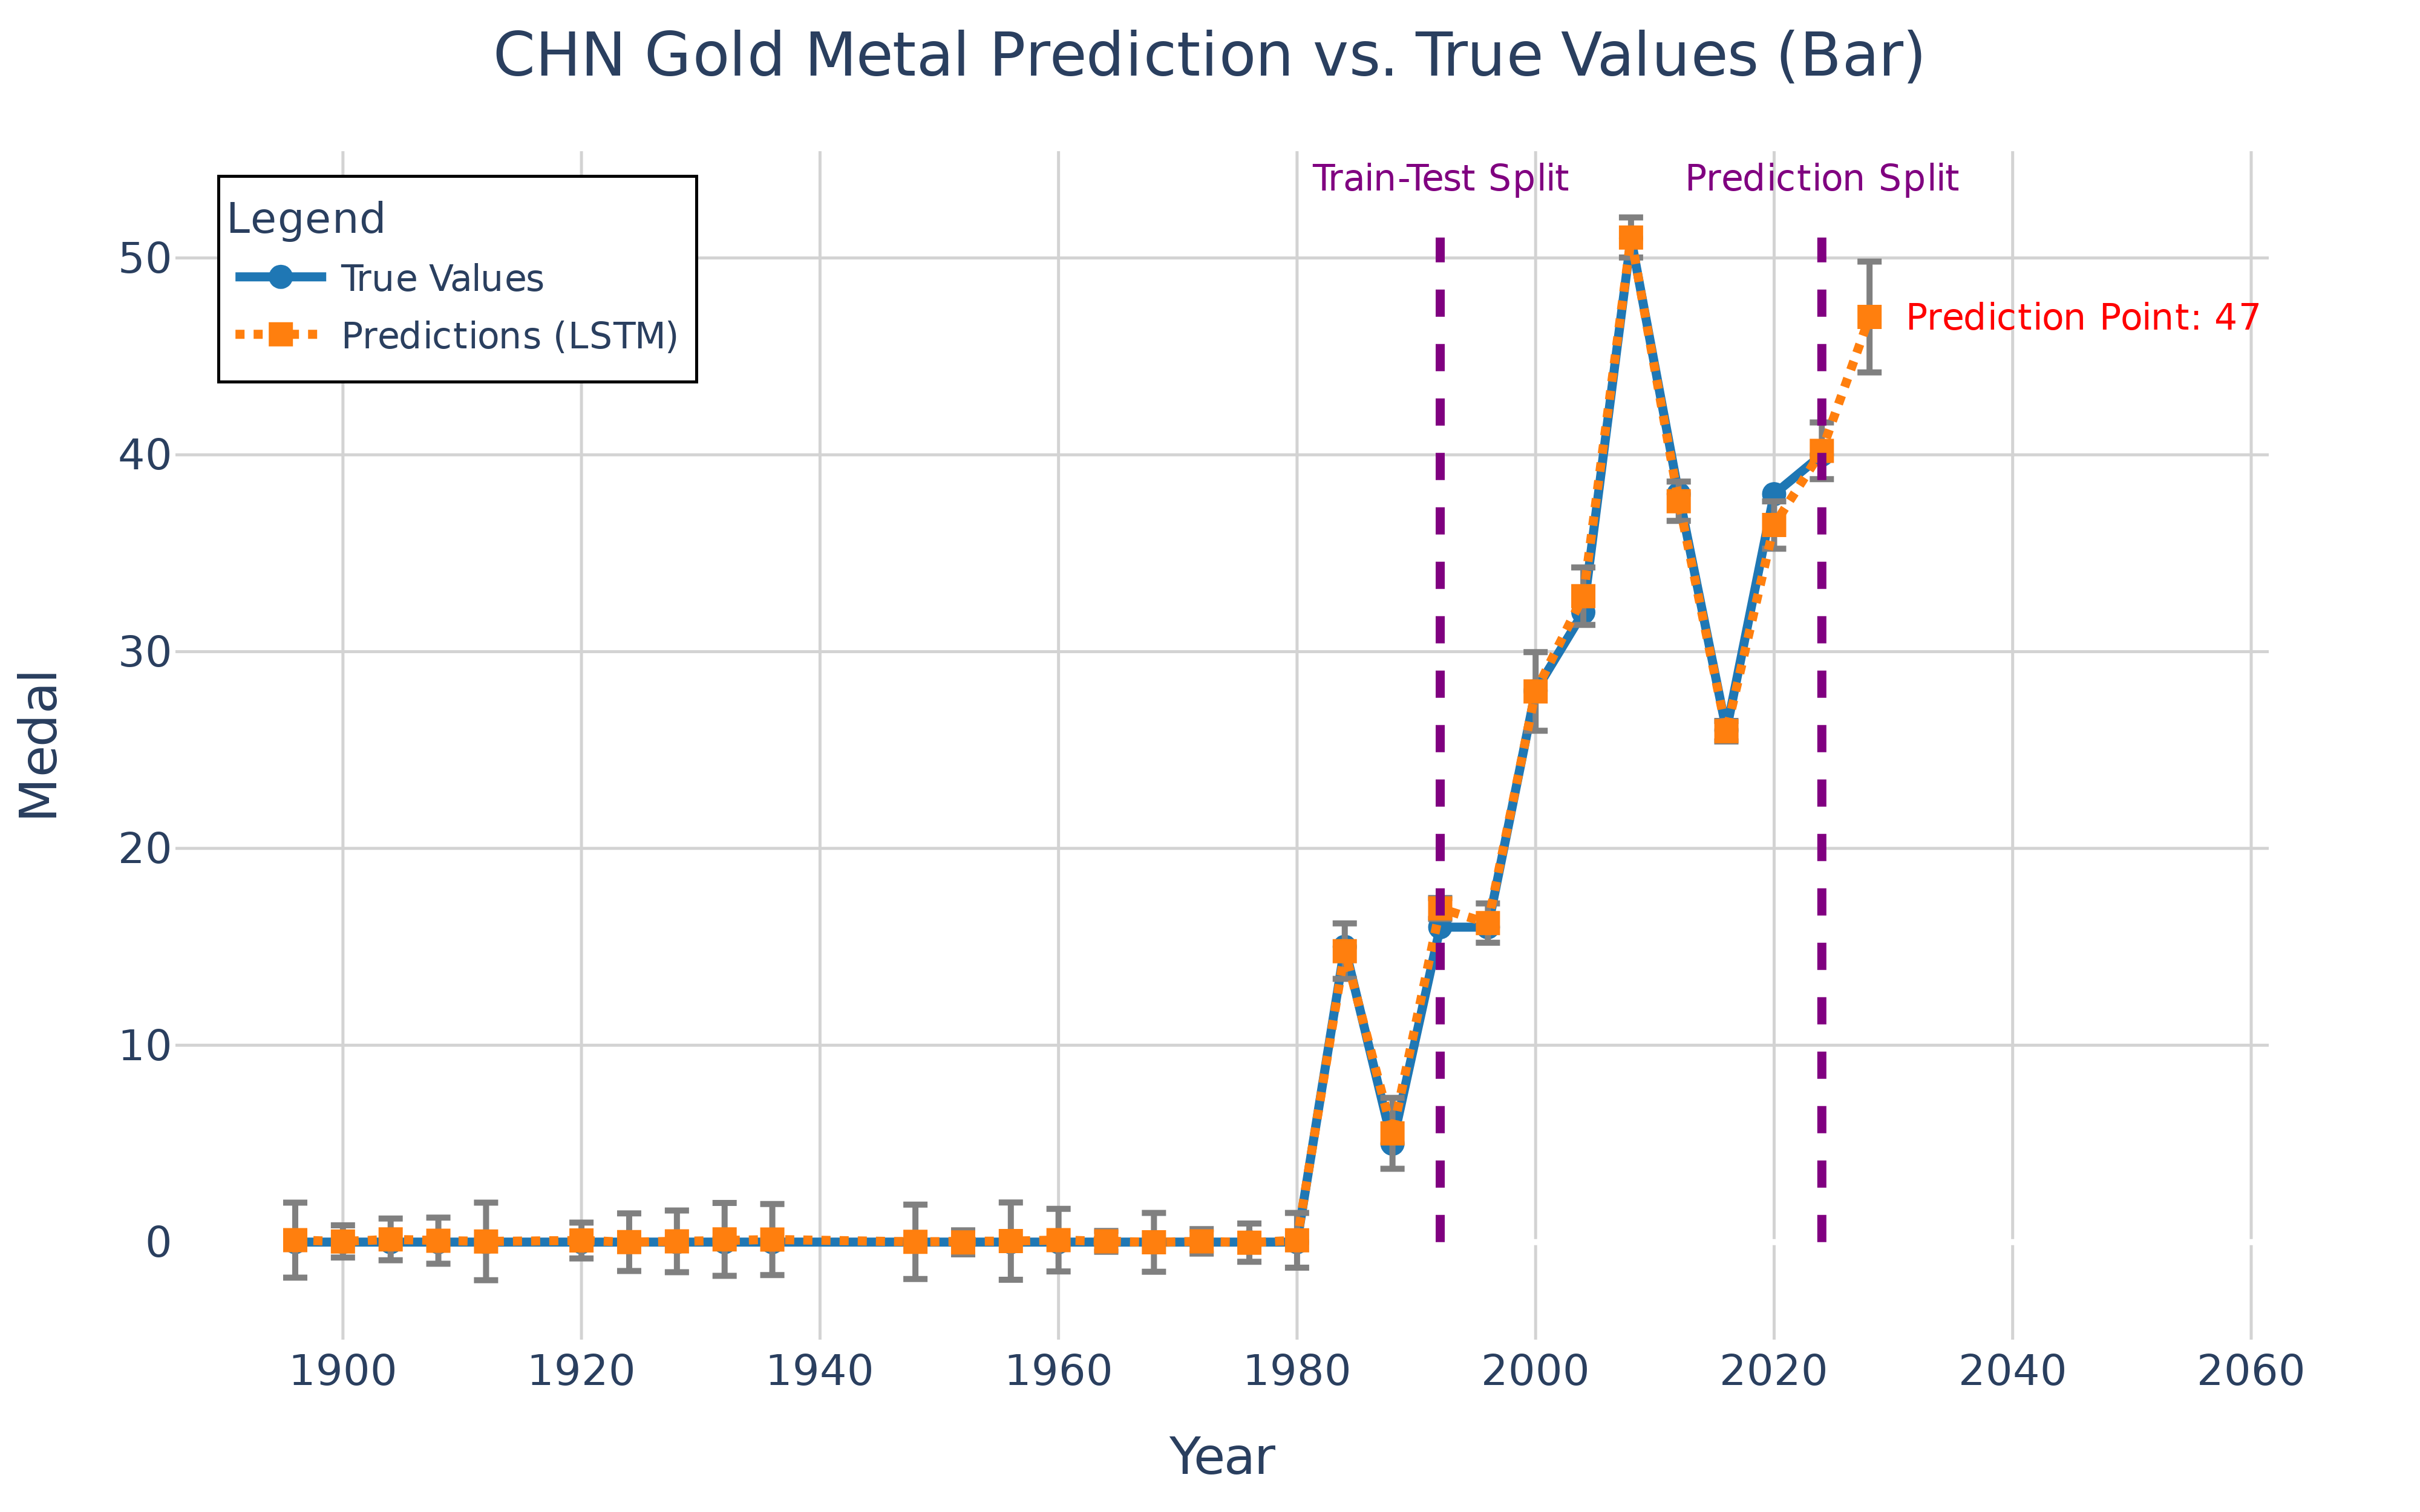
\includegraphics[width=\textwidth]{fig/CHN Gold Metal Prediction vs. True Values (Bar).png}
		\caption{China Gold Medal Prediction Interval}
		\label{fig:chn_gold}
	\end{subfigure}
	\hfill
	\begin{subfigure}[b]{0.48\textwidth}
		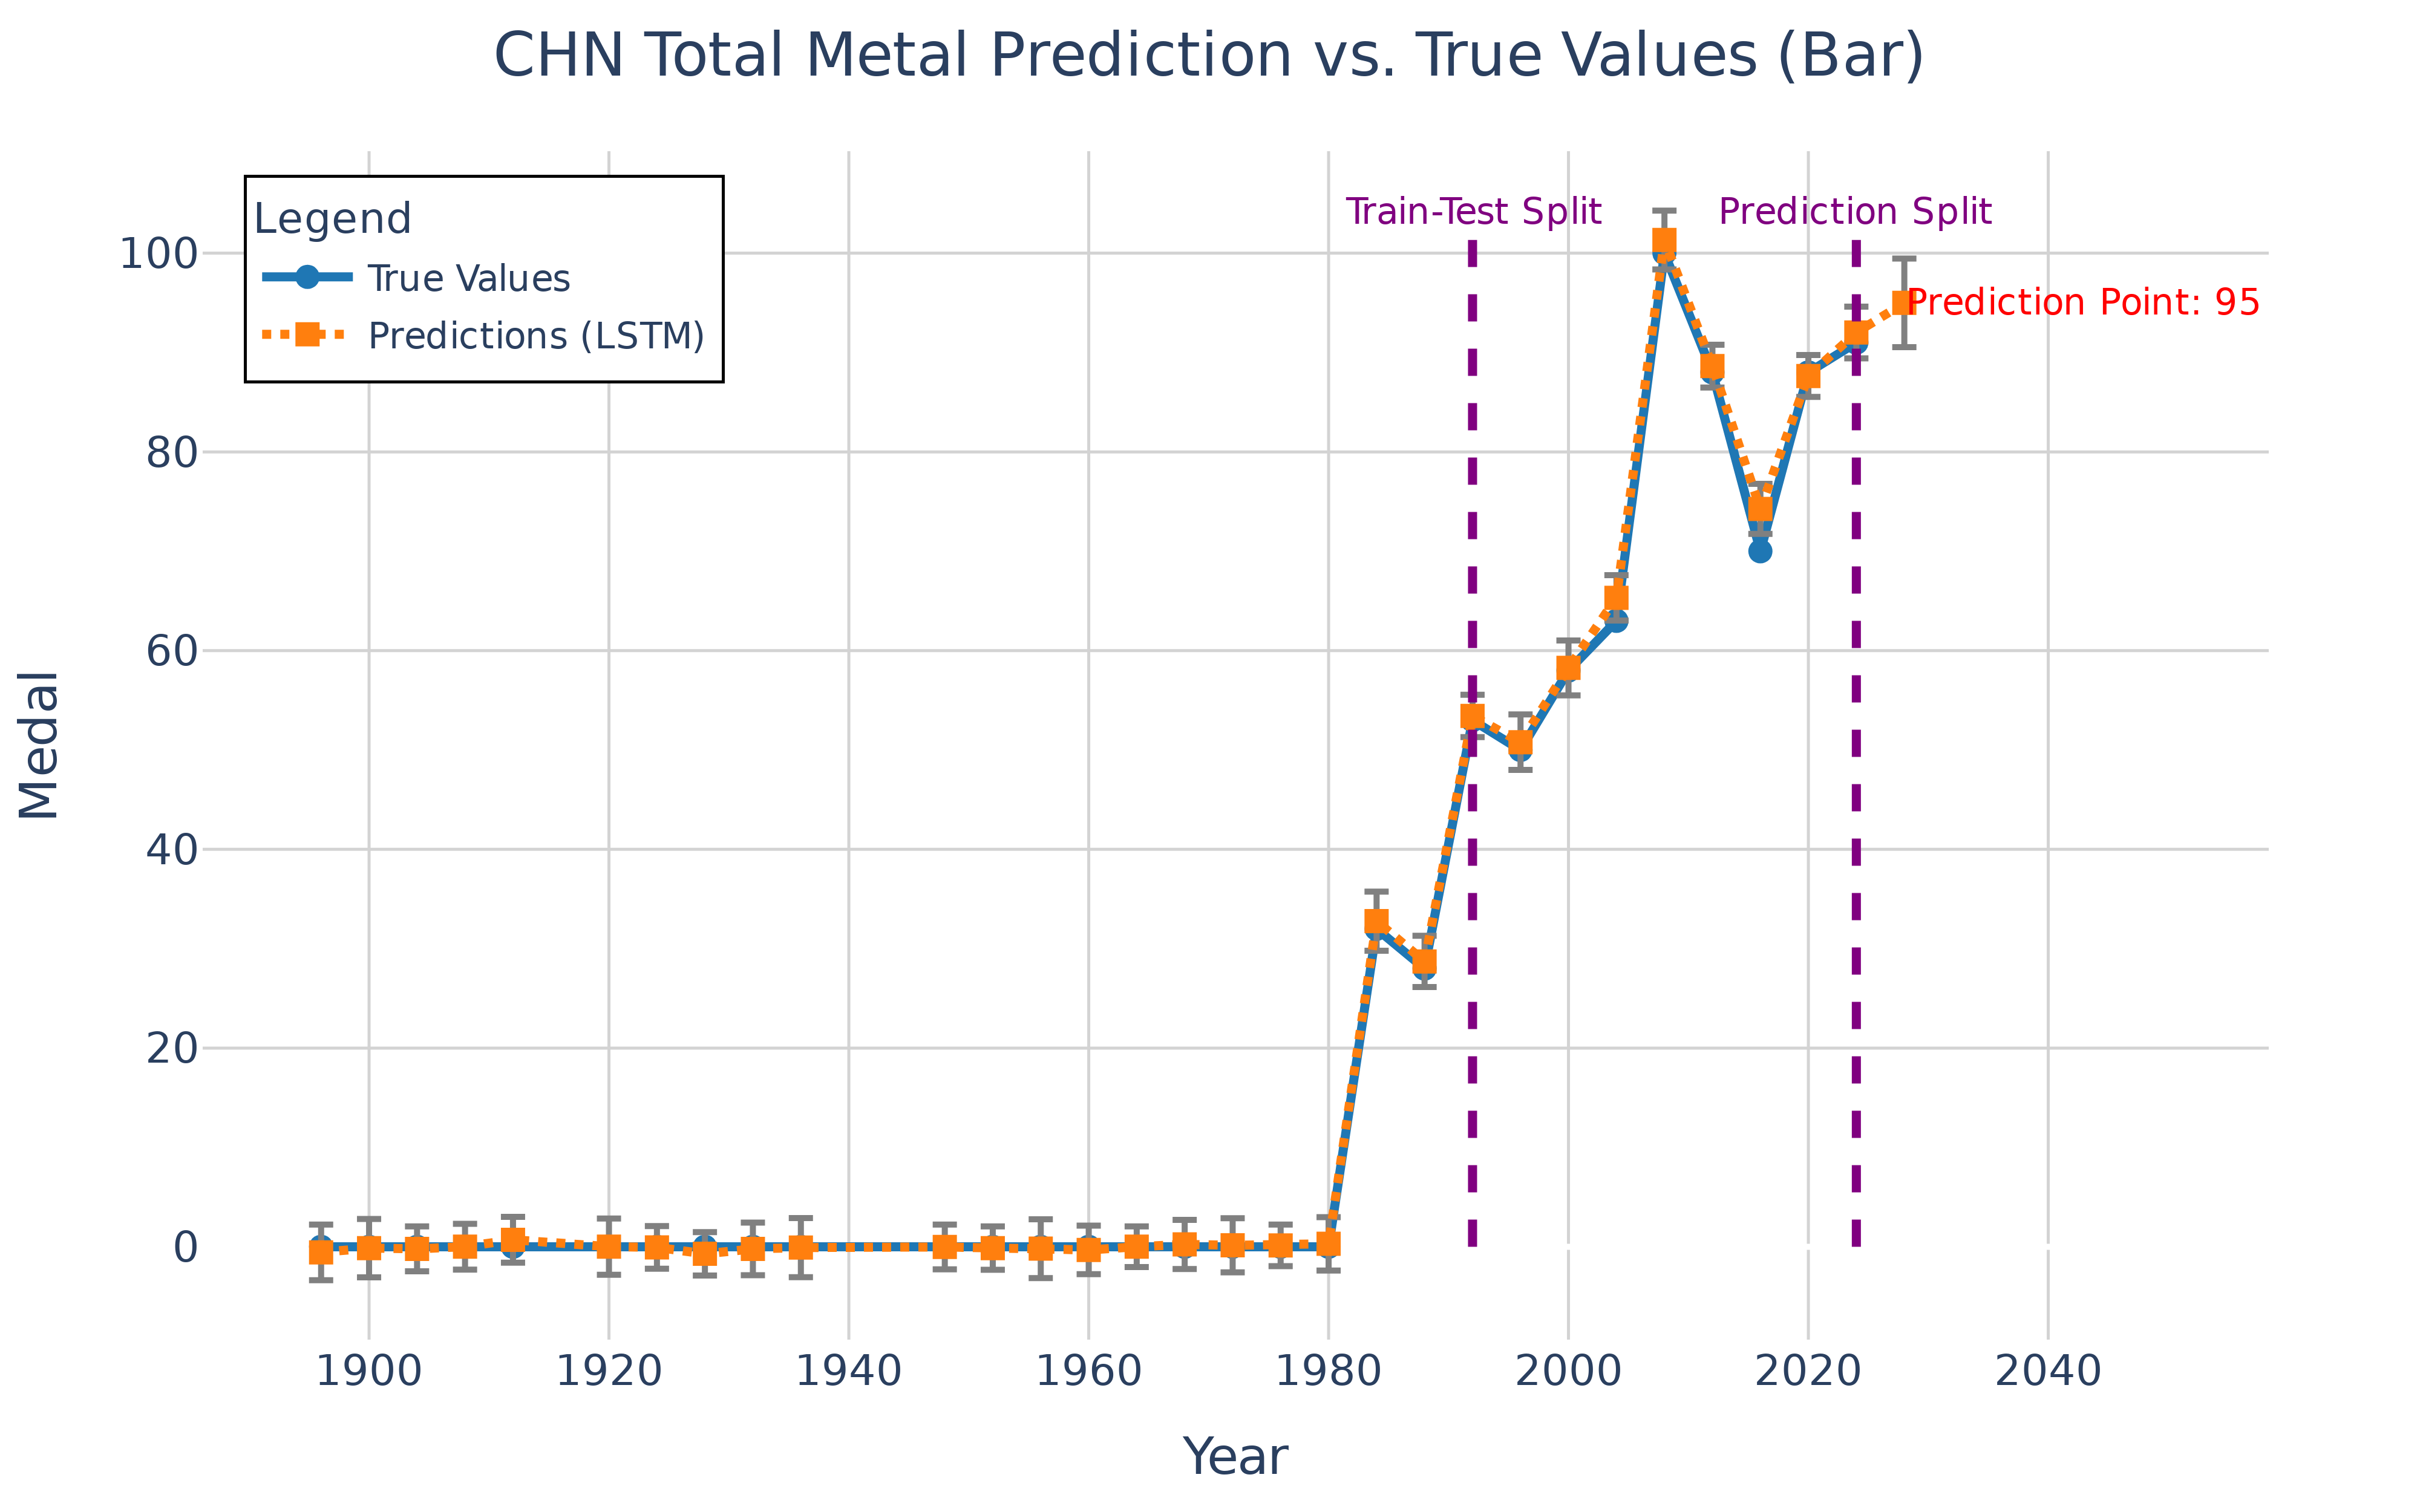
\includegraphics[width=\textwidth]{fig/CHN Total Metal Prediction vs. True Values (Bar).png}
		\caption{China Total Medal Prediction Interval}
		\label{fig:chn_total}
	\end{subfigure}
	
\end{figure}
%\subsubsection{Results Showcase}
The table \ref{12} below shows the total number of medals and gold medals for the predicted top 15 countries with the corresponding prediction intervals.

\begin{table}[H]
	\centering
	\caption{2028 LA Olympics Top 15 Medal and Gold Medal Ranking}
	\label{tab:combined_medals}
	\renewcommand{\arraystretch}{1.2}
	\begin{tabularx}{\textwidth}{l|ccc|ccc}
		\toprule
		\rowcolor{red!10}
		\textbf{Country} & \textbf{Total Medal} & \textbf{Lower} & \textbf{Upper} & \textbf{Gold Medal} & \textbf{Lower} & \textbf{Upper} \\
		\midrule
		\rowcolor{gray!10}
		USA & 128 & 126.0 & 130.0 & 44 & 43.0 & 45.0 \\
		CHN & 95 & 94.0 & 96.0 & 42 & 41.0 & 43.0 \\
		\rowcolor{gray!10}
		GBR & 71 & 69.0 & 73.0 & 37 & 36.0 & 38.0 \\
		GER & 54 & 53.0 & 55.0 & 24 & 23.0 & 25.0 \\
		\rowcolor{gray!10}
		FRA & 51 & 50.0 & 52.0 & 18 & 17.0 & 19.0 \\
		AUS & 46 & 45.0 & 47.0 & 18 & 17.0 & 19.0 \\
		\rowcolor{gray!10}
		JPN & 43 & 42.0 & 44.0 & 16 & 15.0 & 17.0 \\
		RUS & 33 & 32.0 & 34.0 & 15 & 14.0 & 16.0 \\
		\rowcolor{gray!10}
		NED & 33 & 32.0 & 34.0 & 15 & 14.0 & 16.0 \\
		KOR & 28 & 27.0 & 29.0 & 14 & 13.0 & 15.0 \\
		\rowcolor{gray!10}
		ITA & 28 & 27.0 & 29.0 & 14 & 13.0 & 15.0 \\
		ESP & 26 & 25.0 & 27.0 & 13 & 12.0 & 14.0 \\
		\rowcolor{gray!10}
		ROC & 21 & 20.0 & 22.0 & 12 & 11.0 & 13.0 \\
		NZL & 21 & 20.0 & 22.0 & 11 & 10.0 & 12.0 \\
		\bottomrule
	\end{tabularx}
	\label{12}
\end{table}

In Olympic medal prediction, we calculate the probabilities of improvement and decline based on the predicted confidence interval for the 2028 Games. Specifically, the probability of improvement refers to the likelihood that the upper bound of the predicted 2028 medal count exceeds the 2024 medal count, while the probability of decline refers to the likelihood that the lower bound of the predicted 2028 medal count is less than the 2024 medal count.

Let \( MT_{30} \) represent the medal count for a given country in 2024, and let the predicted confidence interval for the 2028 medal count be \([L_{\text{lower}}, L_{\text{upper}}]\). The probabilities of improvement and decline can be expressed by the following formulas:

\textbf{Probability of Improvement}
\[
P_{\text{progress}} = \frac{\max(0, L_{\text{upper}} - MT_{30})}{L_{\text{upper}} - L_{\text{lower}}}
\]
where \( L_{\text{upper}} - M_{T30} \) represents the potential improvement if the 2024 medal count is below the upper bound of the 2028 prediction. If the 2024 medal count exceeds the upper bound, the probability of improvement becomes zero.

\textbf{Probability of Decline} 
\[
P_{\text{decline}} = \frac{\max(0, MT_{30} - L_{\text{lower}})}{L_{\text{upper}} - L_{\text{lower}}}
\]

The following Figure \ref{fig:medal_comparison} illustrates the top five countries that have shown an improvement in their performance at the 2028 Olympic Games in Los Angeles compared to the 2024 Games:


\begin{figure}[h!]
	\centering
	\begin{subfigure}[b]{0.45\textwidth}
		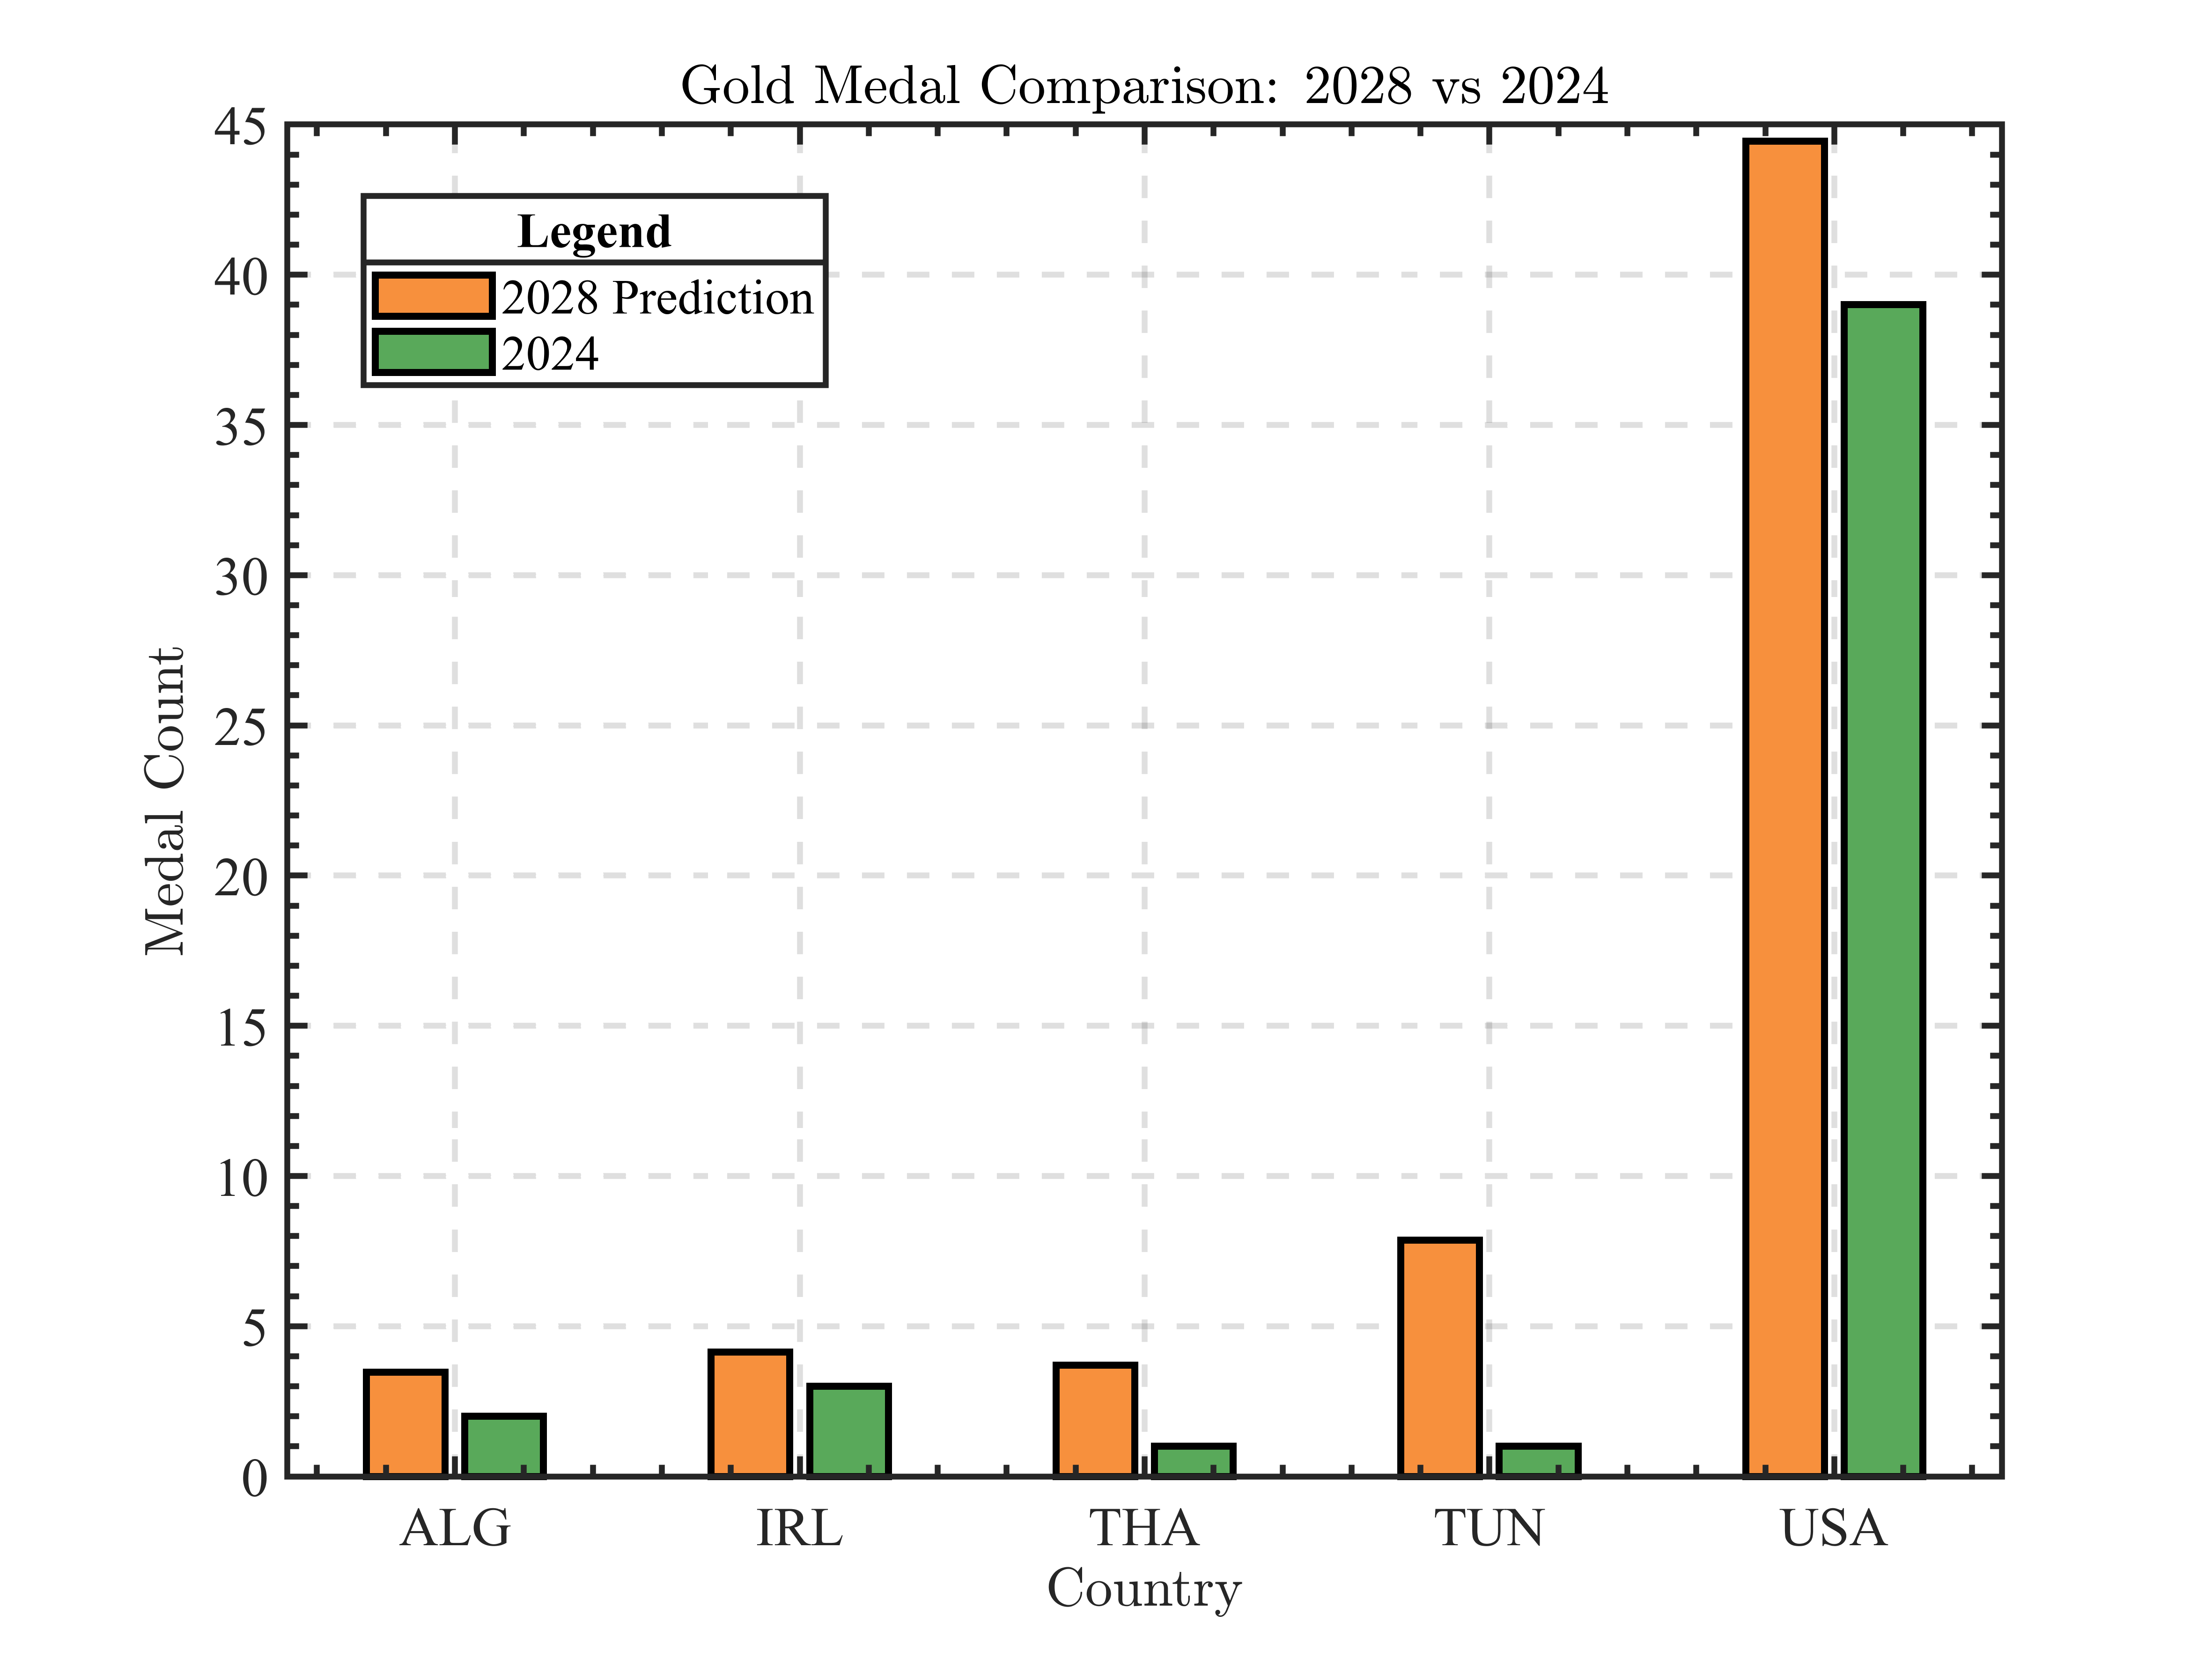
\includegraphics[width=\textwidth]{gold_medal_more_cmp.png}
		\caption{Comparison of Gold Medals: 2028 vs 2024}
		\label{fig:gold_medal}
	\end{subfigure}
	\hfill
	\begin{subfigure}[b]{0.45\textwidth}
		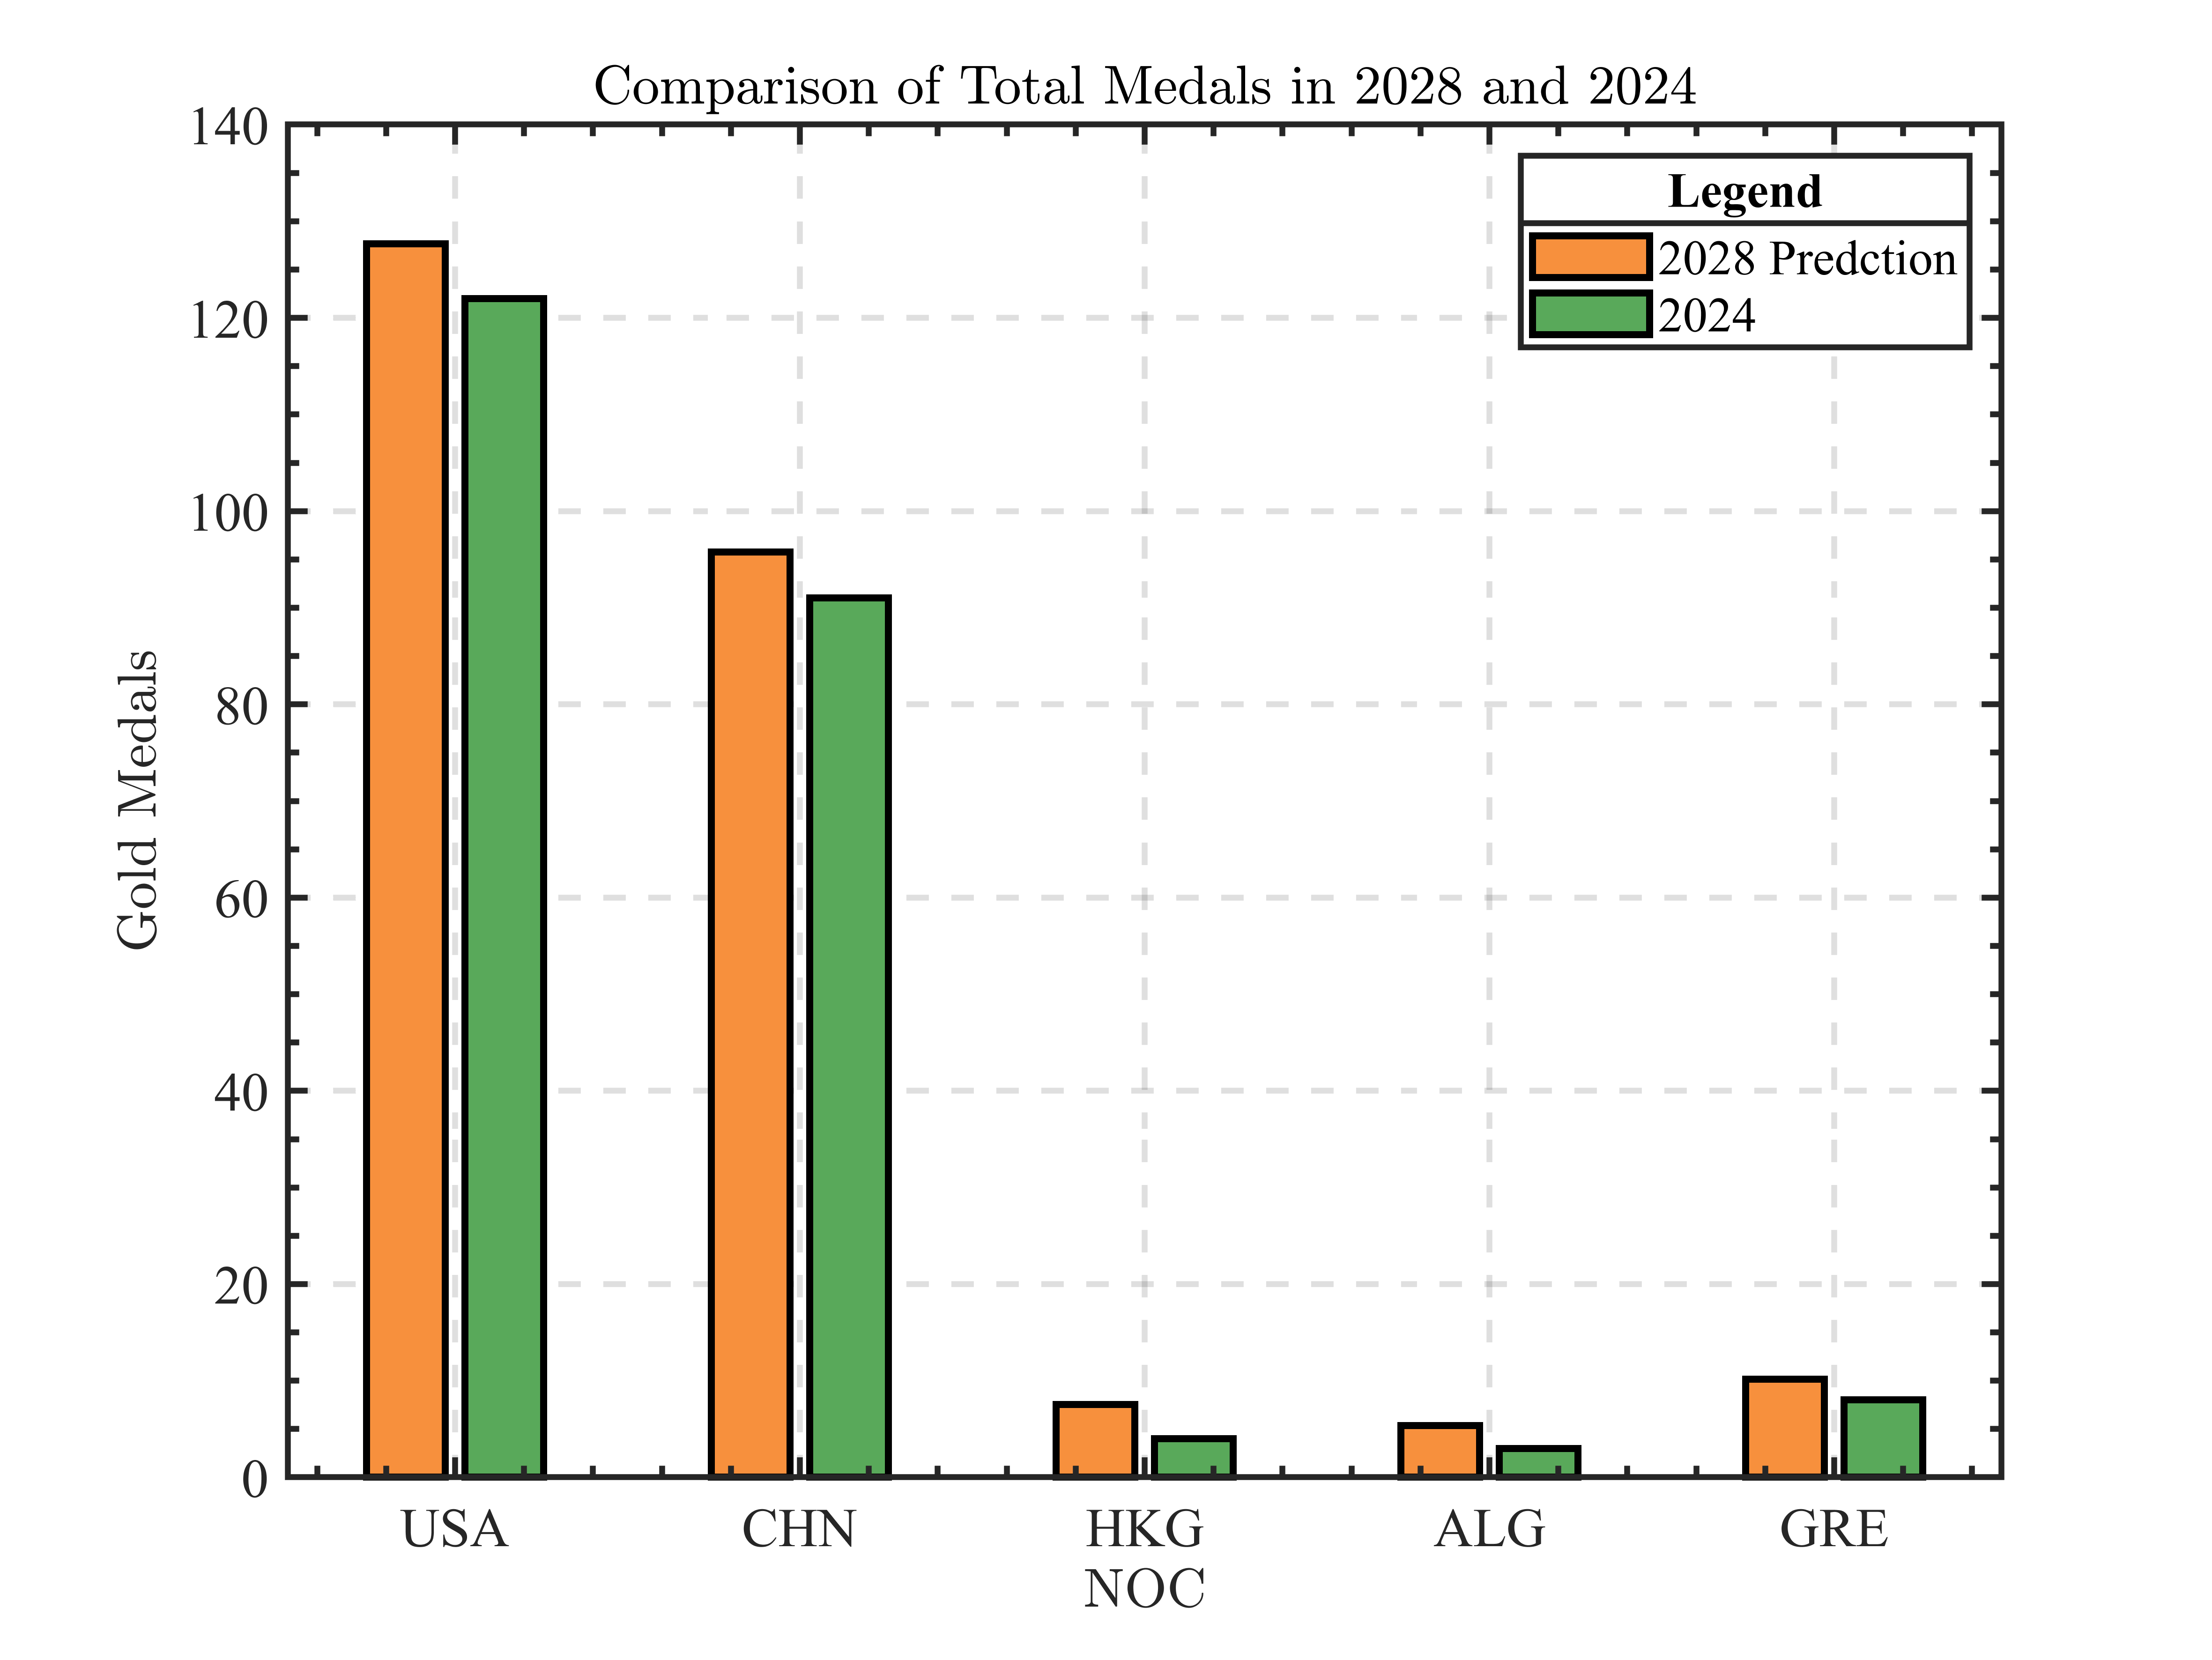
\includegraphics[width=\textwidth]{total_medal_more_cmp.png}
		\caption{Comparison of Total Medals: 2028 vs 2024}
		\label{fig:total_medal}
	\end{subfigure}
	\caption{Top five countries with improved performance at the 2028 Olympic Games}
	\label{fig:medal_comparison}
\end{figure}

The following Figures \ref{fig:medal_comparison1} depict the top five countries that are projected to experience a decline in their performance at the 2028 Olympic Games in Los Angeles compared to the 2024 Games:

\begin{figure}[h!]
	\centering
	\begin{subfigure}[b]{0.45\textwidth}
		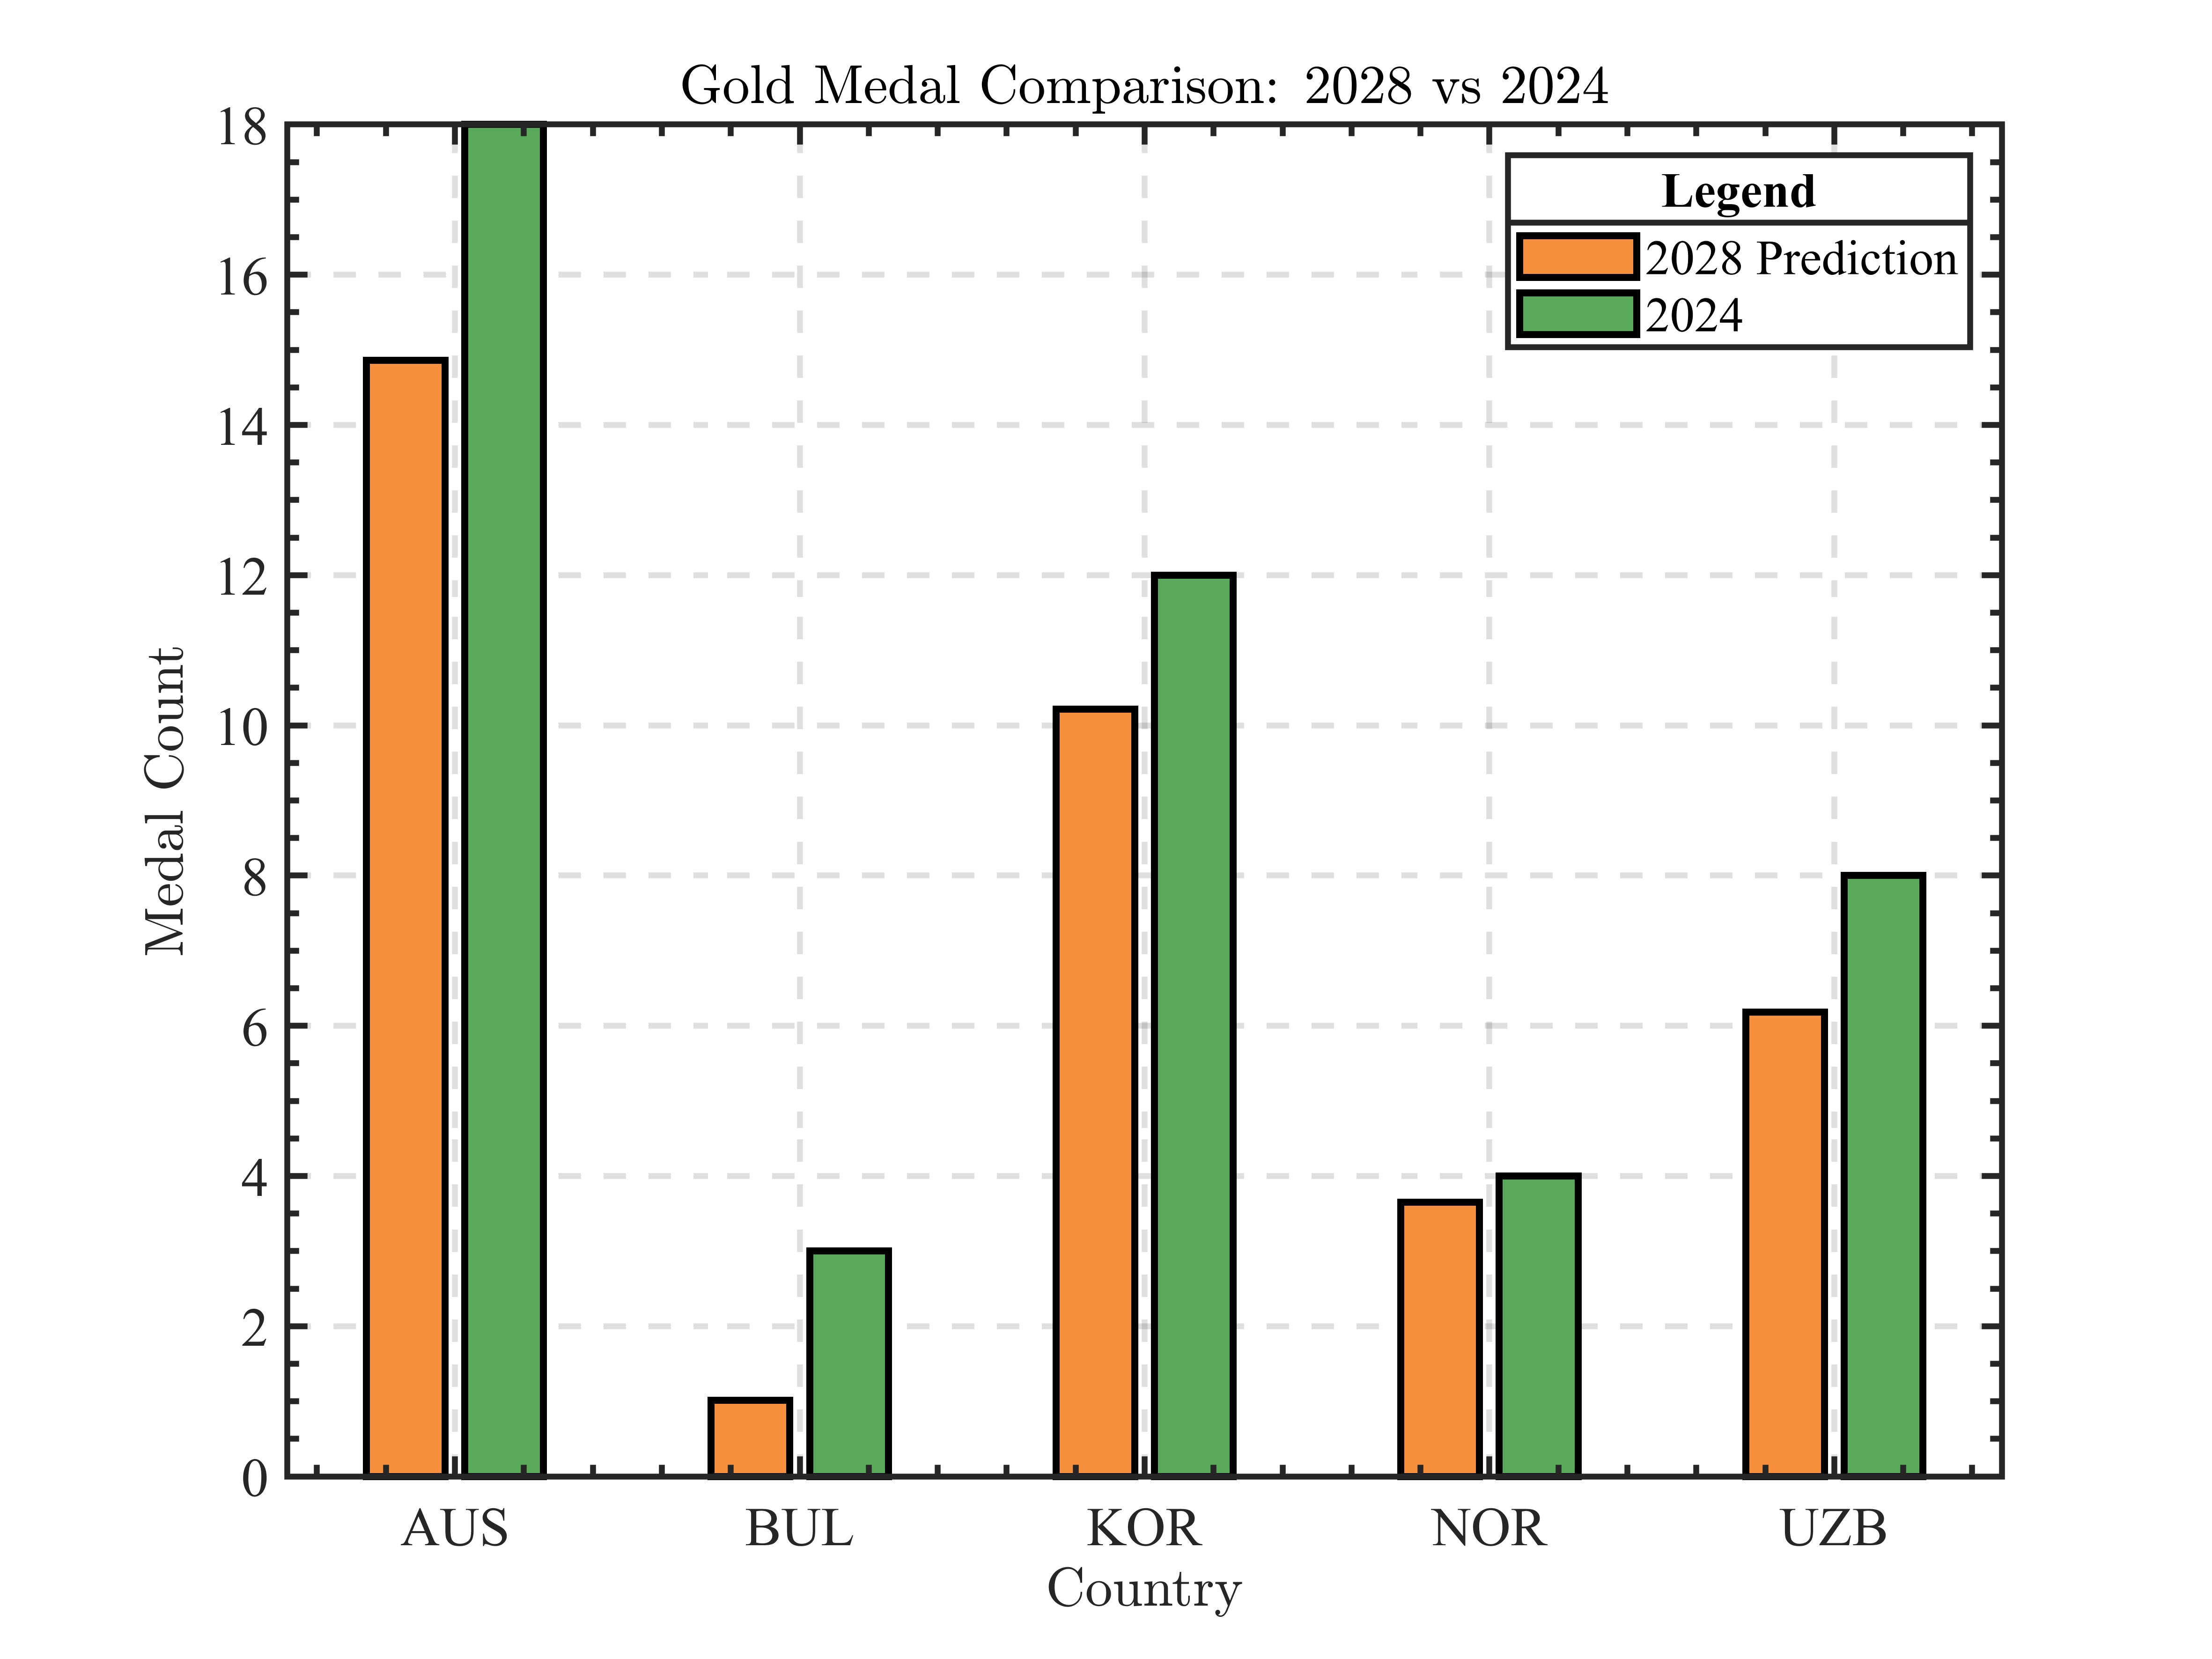
\includegraphics[width=\textwidth]{gold_medal_less_cmp.png}
		\caption{Comparison of Gold Medals: 2028 vs 2024}
		\label{fig:gold_medal1}
	\end{subfigure}
	\hfill
	\begin{subfigure}[b]{0.45\textwidth}
		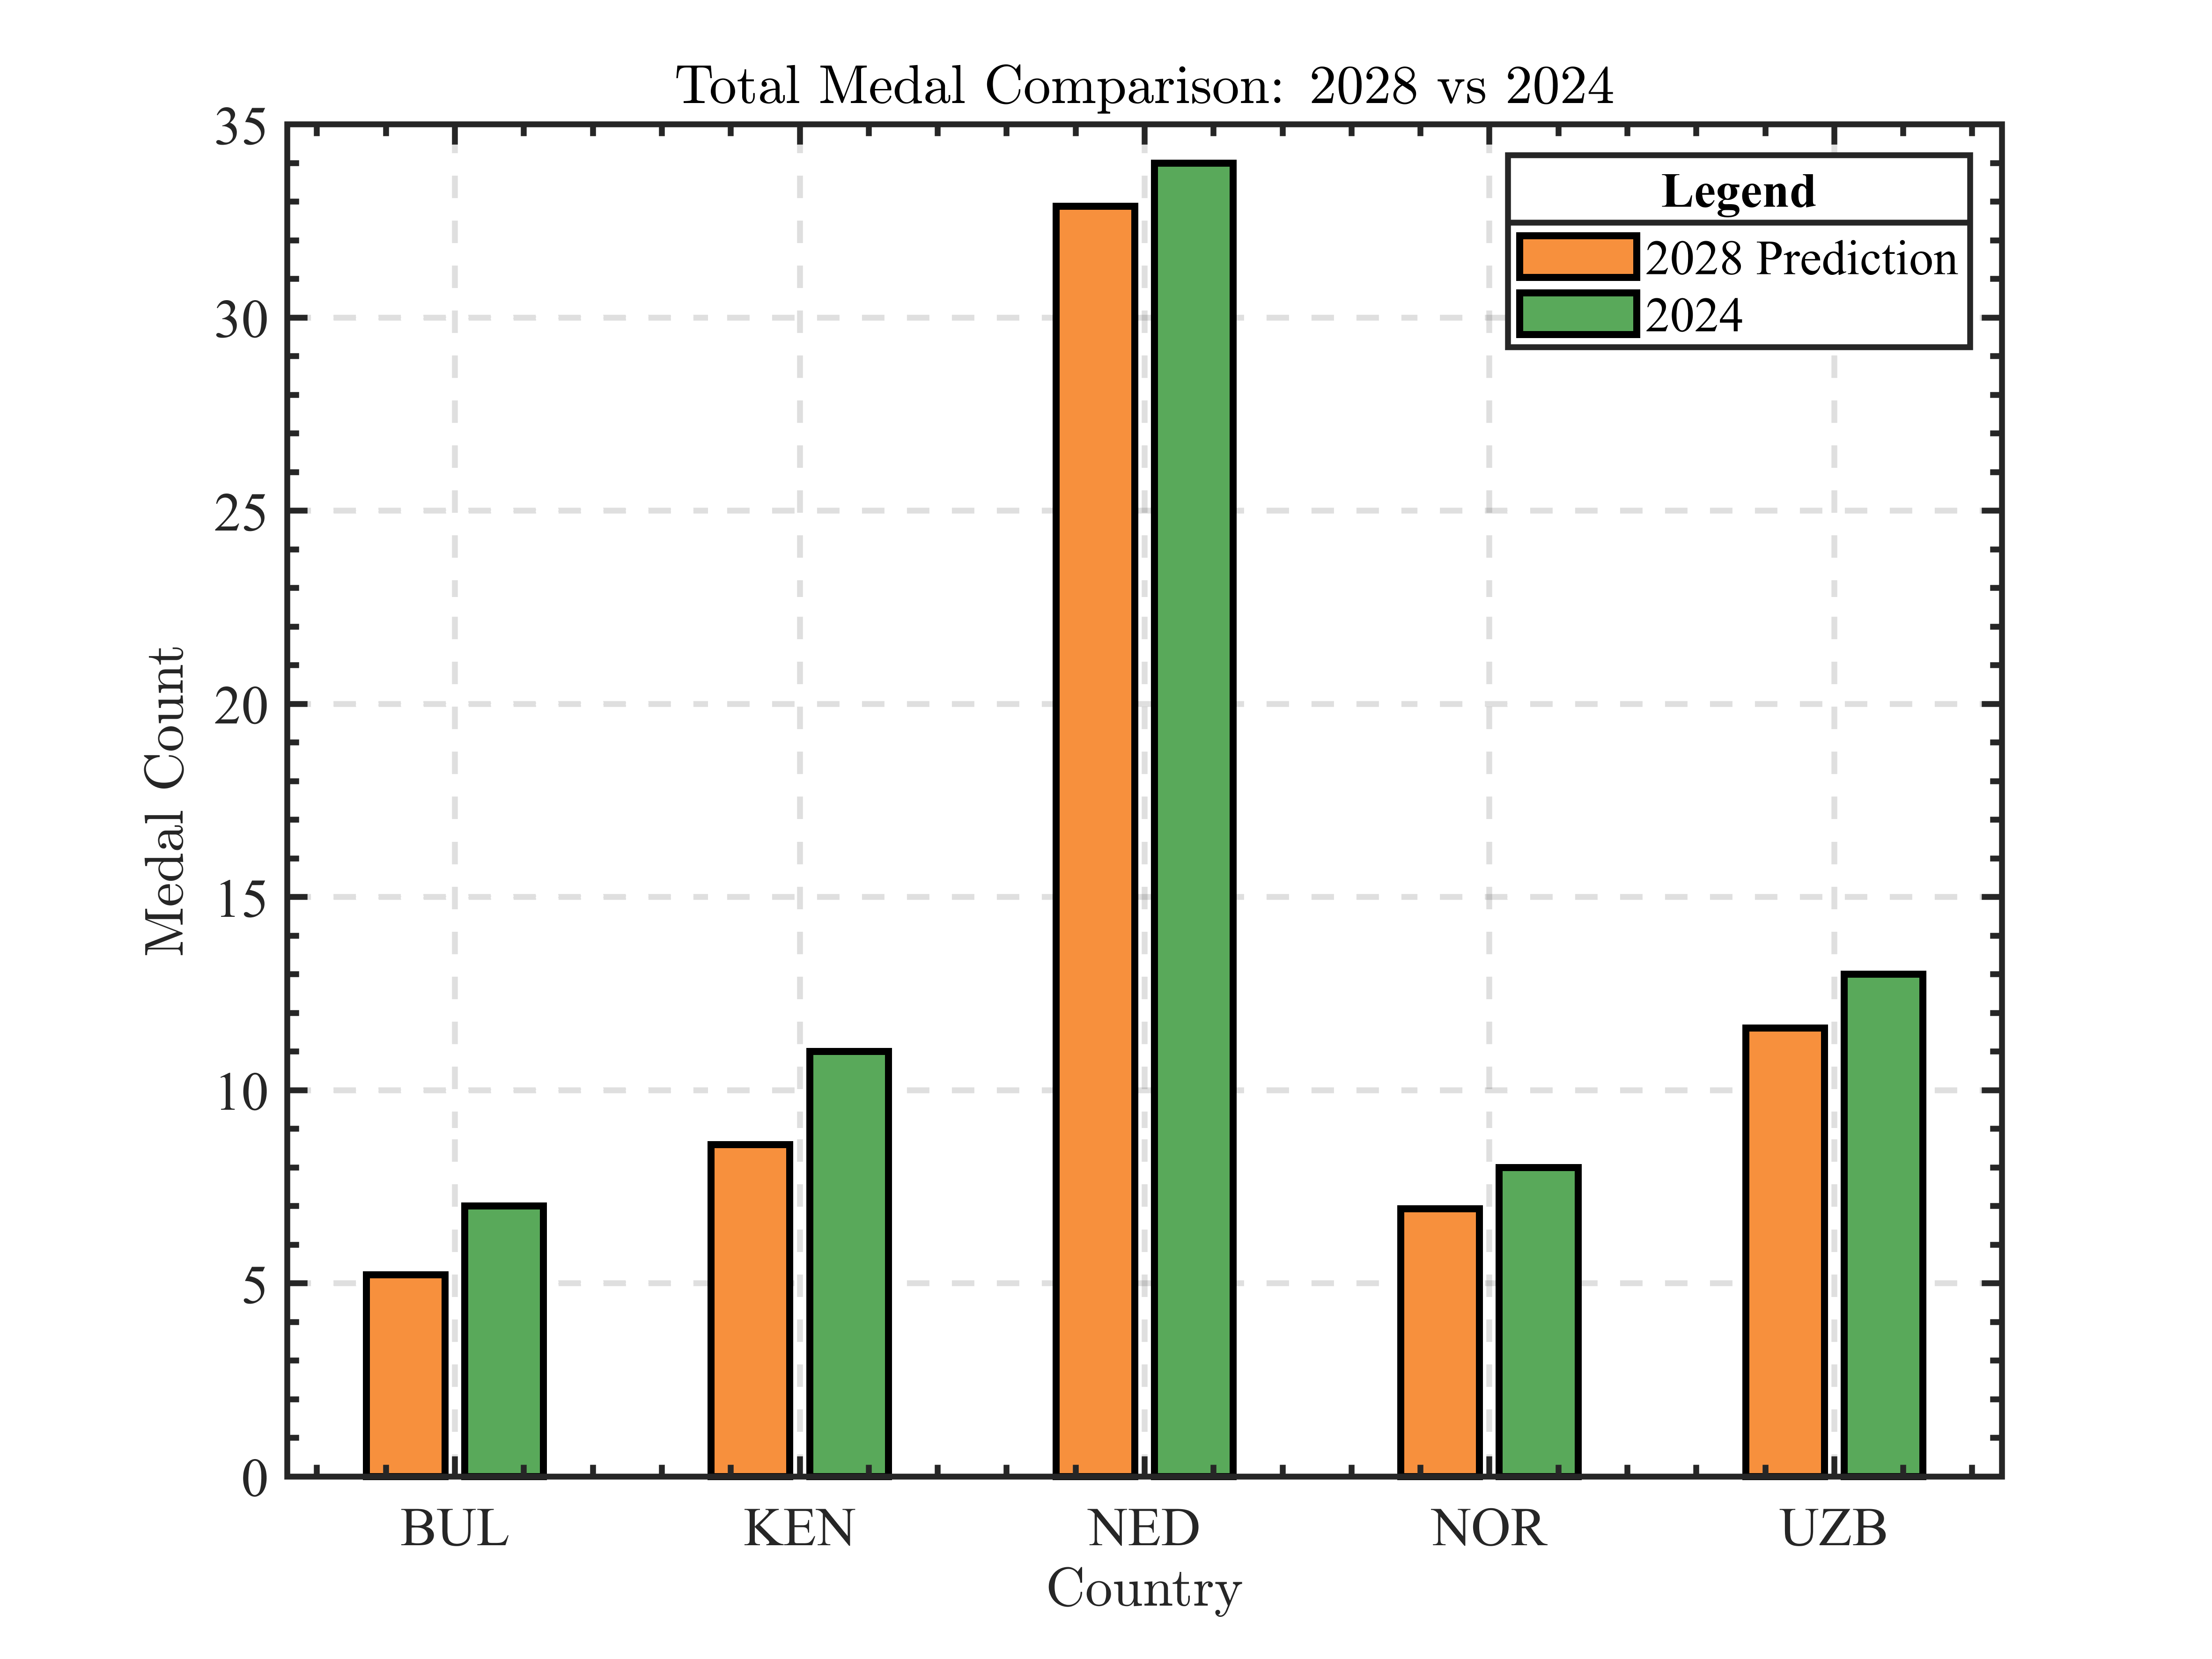
\includegraphics[width=\textwidth]{total_medal_less_cmp.png}
		\caption{Comparison of Total Medals: 2028 vs 2024}
		\label{fig:total_medal1}
	\end{subfigure}
	\caption{Top five countries with a decline in achievement at the 2028 Olympic Games}
	\label{fig:medal_comparison1}
\end{figure}

\subsubsection{Modelling Assessment}

% Model Performance Table
\begin{table}[H]
	\centering
	\caption{LSTM Model Performance Evaluation (Training/Test Set Comparison)}
	\label{tab:model_performance}
	\begin{tabular}{lrrp{8cm}}
		\toprule
		\rowcolor{red!10}
		\textbf{Metric} & \textbf{Train} & \textbf{Test} & \textbf{Analysis} \\
		\midrule
		\rowcolor{gray!10}
		MSE  & 0.9836 & 1.1284 & Small train/test error gap ($\Delta$=0.1448) indicates mild overfitting with preserved generalization capability \\
		RMSE & 0.9918 & 1.0625 & Prediction std dev ≈1 gold medal, meeting competition forecasting precision requirements \\
		\rowcolor{gray!10}
		MAE  & 0.7571 & 0.8923 & Mean absolute error <1 gold medal validates prediction reliability \\
		R²   & 0.9844 & 0.9216 & Explains 92.16\% data variance, demonstrating superior nonlinear pattern capture \\
		\bottomrule
	\end{tabular}
\end{table}

\begin{figure}[H]
	\centering
	\begin{adjustbox}{minipage=0.5\textwidth,valign=t}
		\centering
		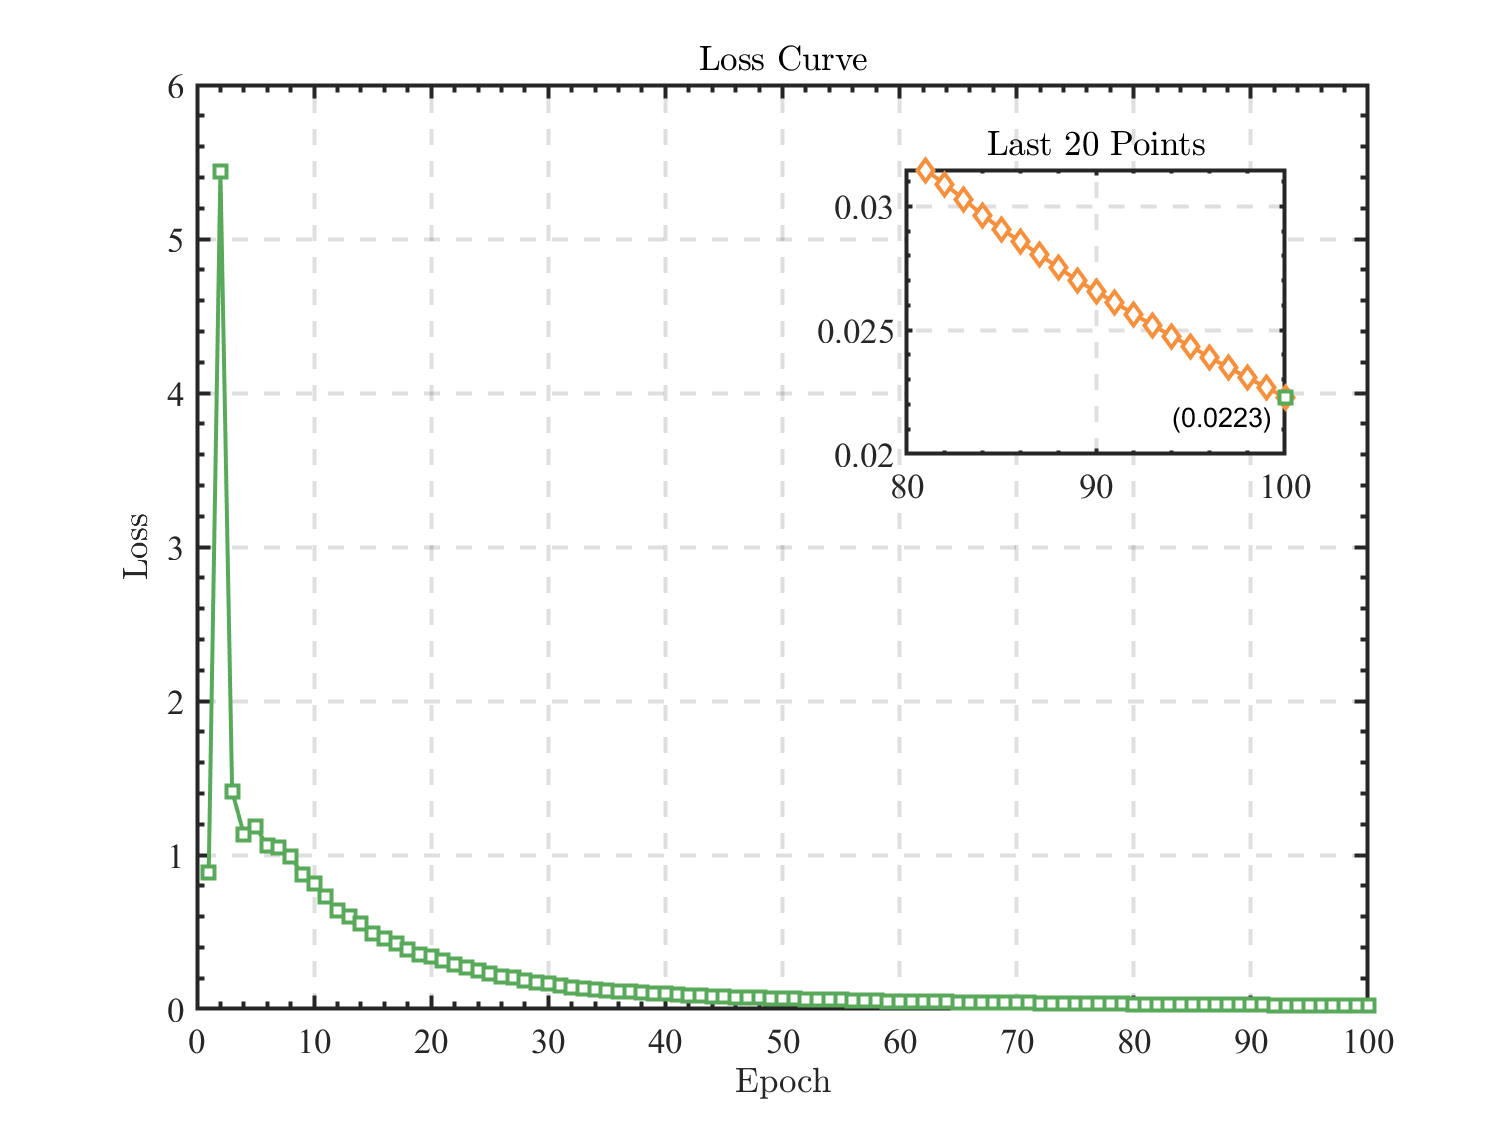
\includegraphics[width=\linewidth]{fig/loss.png}
		\caption{LSTM Training Loss Curve with Monte Carlo Dropout}
		\label{fig:training_curve}
	\end{adjustbox}
	\hfill
	\begin{adjustbox}{minipage=0.45\textwidth,valign=t}
		\vspace*{-1.2ex} % 精确垂直对齐补偿
		\begin{itemize}
			\item \textbf{Rapid Convergence Phase \\(0--5 epochs)}: 
			Loss drops from 0.03 to 0.025 with synchronized validation loss reduction, demonstrates rapid learning of underlying patterns
			
			\item \textbf{Stabilized Optimization Phase \\(5--20 epochs)}: 
			Training loss ($\downarrow$0.0229$\rightarrow$0.00) and validation loss ($\downarrow$0.025$\rightarrow$0.00) co-converge, suggesting appropriate dropout rate (estimated 0.2)
			
			\item \textbf{Final Convergence State \\(>20 epochs)}: 
			Dual loss curves stabilize near 0.00 with $\pm$0.001 fluctuations, indicating optimal model state
		\end{itemize}
	\end{adjustbox}
\end{figure}
%\begin{figure}[H]
%	\centering
%	\begin{minipage}{0.45\textwidth}
%		\centering
%		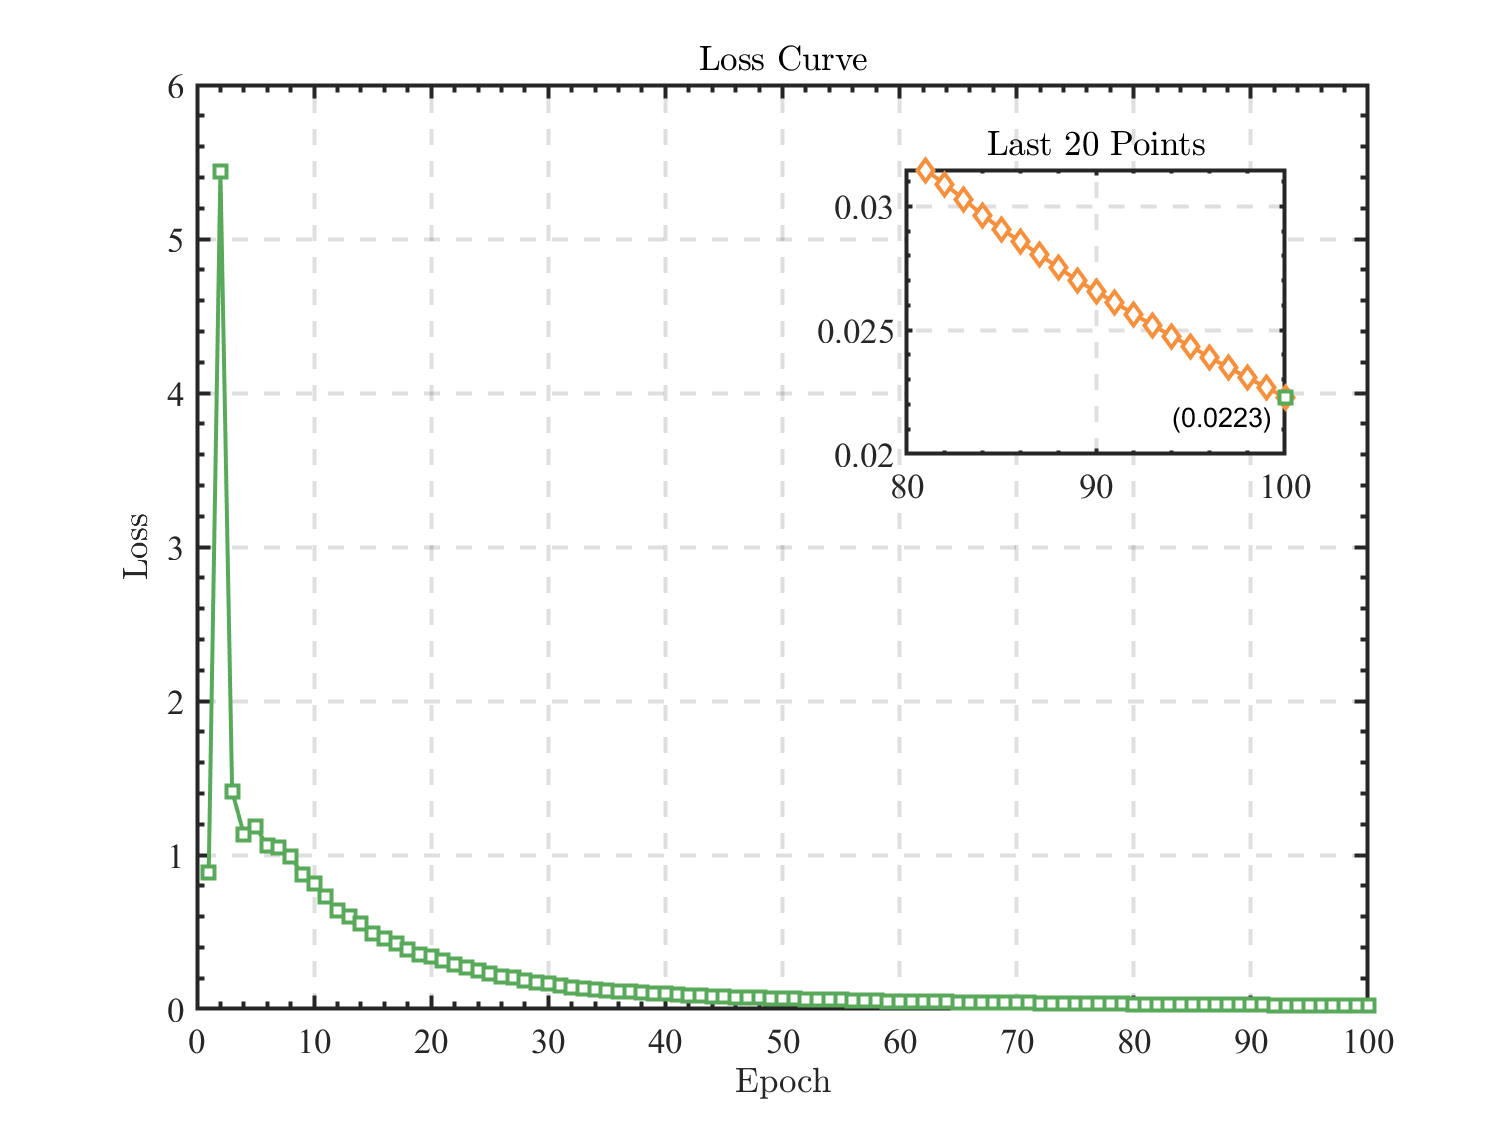
\includegraphics[width=\linewidth]{fig/loss.png}
%		\label{fig:loss}
%	\end{minipage}
%	\begin{minipage}{0.45\textwidth}
%		\centering
%		\label{tab:usa_eval}
%		\begin{tabular}{lrr}
%			\toprule
%			\rowcolor{red!10}
%			\textbf{Metric} & \textbf{Training Set} & \textbf{Test Set} \\
%			\midrule
%			\rowcolor{gray!10}
%			MSE          & 0.9836 & 1.1284 \\
%			RMSE         & 0.9918 & 1.0625 \\
%			\rowcolor{gray!10}
%			MAE          & 0.7571 & 0.8923 \\
%			R²           & 0.9844 & 0.9216 \\
%			\bottomrule
%		\end{tabular}
%	\end{minipage} \hfill
%
%	\caption{Flow of LSTM based on Monte Carlo Dropout}
%\end{figure}



\subsection{ Prediction of Maiden Medal for Medal-Less Countries}
The objective of this model is to predict whether countries that have never won a medal in the past (i.e., "first-time winning countries") will be able to win a medal in future Olympic Games. Traditional medal prediction models, which usually rely on historical medal data, may not effectively predict the future performance of these countries. Therefore, additional factors, such as the host country effect, athlete participation growth, and the addition of new events, need to be considered.

\subsubsection{Index Analysis}

\begin{itemize}[leftmargin=0.15in, labelsep=0.1in, itemsep=1pt, parsep=0pt]
	\item \textbf{Target Variable}
	
	The target variable is defined as:
	\[
	y(t,i) = 
	\begin{cases} 
		1, & \text{if country } i \text{ wins a medal in year } t, \\ 
		0, & \text{otherwise.}
	\end{cases}
	\]
	
	\item \textbf{Participants Growth Rate (PGR)}
	
	Define \(\Delta N(k,i) \equiv N_{\text{athletes}}(k-1,i) - N_{\text{athletes}}(k,i)\), the growth rate is:
	\[
	\text{PGR}(t,i) = \frac{1}{2} \left[ \max(0, \Delta N(t-1,i)) + \max(0, \Delta N(t-2,i)) \right]
	\]
	where \(k\) denotes the year index. Negative growth values are automatically clipped by the \(\max(0,\cdot)\) operator.
	
	\item \textbf{New Project Index (NPI)}
	
	Counts newly introduced Olympic projects in recent editions:
	\[
	\text{NPI}(t,i) = \sum_{k=t-3}^{t-1} \mathbf{1}\left( P(k,i) \cap \neg P(t-4, i) \right)
	\]
	where \( P(k, i) \) represents the set of projects in edition \( k \) for country \( i \), the indicator function \( \mathbf{1}(\cdot) \) takes the value 1 when the condition inside is true, and 0 otherwise, and the operator \(\neg\) represents negation.
	
	\item \textbf{Unpopular Project Participation Growth Rate (LPIR)}
	
	Define \(\Delta N(k,i) \equiv N_{\text{unpopular}}(k,i) - N_{\text{unpopular}}(k-1,i)\), the growth rate is:
	\[
	\text{LPIR}(t,i) = \frac{1}{2} \left[ \max(0, \Delta N(t-1,i)) + \max(0, \Delta N(t-2,i)) \right]
	\]
\end{itemize}


\subsubsection{XGBoost 01 Breakthrough in Olympic Medal Prediction}

We utilize an XGBoost classifier to predict the probability of first-time medal wins for countries. The model’s input is the feature vector for country \( i \) at time \( t \), denoted as \( X(t,i) \):

\[
X(t,i) = [PGR(t,i), NPI(t,i), LPIR(t,i)]
\]

The XGBoost classifier is an ensemble method based on decision trees, where each tree contributes to the final prediction. The final prediction is the weighted sum of the outputs from all trees in the model:

\[
P(\text{Medal}(t,i)) = \sum_{k=1}^{K} \alpha_k \cdot f_k(X(t,i))
\]

where \( K \) is the number of trees, \( \alpha_k \) is the weight of the \( k \)-th tree, and \( f_k(\cdot) \) is the decision function of the \( k \)-th tree.


For countries that have not previously won any medals, the XGBoost classifier calculates the probability of winning a medal in the next Olympic Games. If the predicted probability exceeds a predefined threshold, the model predicts that the country has the potential to win a first medal:

\[
P_{\text{Medal}}(t,i) > \text{Threshold}
\]

The specific algorithm flow is shown below.
\begin{algorithm}[H]
	\caption{XGBoost for Breakthrough Prediction}
	\label{alg:xgboost_short}
	\begin{algorithmic}[1]
		\Require 
		$X$: Feature matrix (PGR, NPI, LPIR) \\
		$y$: Binary target vector \\
		$\mathit{test\_ratio} \in (0,1)$
		
		\Procedure{Model Pipeline}{}
		\State $(X_{\mathit{tr}}, X_{\mathit{te}}, y_{\mathit{tr}}, y_{\mathit{te}}) \gets \texttt{split}(X, y, \mathit{test\_ratio})$
		\State $\mathit{model} \gets \texttt{XGBClassifier}(n\_est=100, \eta=0.1, d_{max}=3)$
		\State $\mathit{model}.\texttt{fit}(X_{\mathit{tr}}, y_{\mathit{tr}})$
		
		\State $\hat{y} \gets \mathit{model}.\texttt{predict}(X_{\mathit{te}})$
		\State $p_{\mathit{prob}} \gets \mathit{model}.\texttt{predict\_proba}(X_{\mathit{te}})$
		
		\State Evaluate: $\mathit{Acc} \gets \frac{\mathit{TP+TN}}{n}$, $\mathit{AUC} \gets \int \mathit{ROC}$
		\State Plot: ROC curve, Confusion Matrix, Feature Importance
		\EndProcedure
	\end{algorithmic}
\end{algorithm}

	
Drawing on the XGBoost model's results, we identify the top 10 countries with the highest probability of securing their first Olympic medal. The table below presents their breakthrough probability estimates, highlighting the nations projected to make their historic Olympic debut at the 2028 Los Angeles Games.
\begin{table}[H]
	\centering
	\setlength{\tabcolsep}{25pt} % Adjust column separation to increase width
	\begin{tabular}{ccccc}
		\toprule
		\rowcolor{red!10} 
		\textbf{NOC} & \textbf{pgr} & \textbf{npi} & \textbf{lpir} & \textbf{predicted\_probability} \\ 
		\midrule
		\rowcolor{gray!10}
		FSM & 1.0 & 19 & 0.0 & 0.85 \\ 
		\rowcolor{white}
		AND & 1.0 & 19 & 0.0 & 0.78 \\ 
		\rowcolor{gray!10}
		PLW & 1.0 & 19 & 0.0 & 0.72 \\ 
		\rowcolor{white}
		BRU & 0.5 & 19 & 0.0 & 0.65 \\ 
		\rowcolor{gray!10}
		CAY & 0.5 & 19 & 0.0 & 0.58 \\ 
		\rowcolor{white}
		GBS & 1.0 & 19 & 0.0 & 0.52 \\ 
		\rowcolor{gray!10}
		BAN & 0.5 & 19 & 0.0 & 0.47 \\ 
		\rowcolor{white}
		LAO & 1.5 & 19 & 0.0 & 0.42 \\ 
		\rowcolor{gray!10}
		GUI & 0.5 & 19 & 0.0 & 0.38 \\ 
		\rowcolor{white}
		PLE & 1.0 & 19 & 0.0 & 0.37 \\ 
		\bottomrule
	\end{tabular}
	\caption{Predicted Probability of Winning First Olympic Medal}
	\label{tab:predicted_probability}
\end{table}

\subsubsection{Modelling Assessment}
\begin{table}[H]
	\centering
	\begin{tabular}{c c c c c}
		\toprule
		\rowcolor{red!10} \textbf{Metric} & \textbf{Class 0} & \textbf{Class 1} & \textbf{Macro Avg} & \textbf{Weighted Avg} \\ 
		\midrule
		\rowcolor{gray!10} Accuracy & 0.83 & 0.87 & 0.85 & 0.85 \\
		\rowcolor{white} Precision & 0.88 & 0.82 & 0.85 & 0.85 \\
		\rowcolor{gray!10} Recall & 0.83 & 0.87 & 0.85 & 0.85 \\
		\rowcolor{white} F1-Score & 0.85 & 0.84 & 0.85 & 0.84 \\
		\rowcolor{gray!10} ROC-AUC & 0.90 & 0.90 & 0.90 & 0.90 \\
		\bottomrule
	\end{tabular}
	\caption{Optimized XGBoost Model Evaluation Metrics}
	\label{tab:model_metrics}
\end{table}

The optimized XGBoost model demonstrates strong performance, achieving an overall \textbf{accuracy of 85\%} and a high \textbf{ROC-AUC score of 0.90}, indicating excellent class discrimination. Precision is particularly strong for Class 0 (\textbf{88\%}), while Class 1 precision is slightly lower at \textbf{82\%}, suggesting some room for improvement in minimizing false positives. Recall values are balanced, with \textbf{87\% for Class 1} and \textbf{83\% for Class 0}, showing the model effectively identifies most true positives but may miss a few Class 0 instances. The F1-scores of \textbf{0.85 (Class 0)} and \textbf{0.84 (Class 1)} further confirm a well-balanced trade-off between precision and recall, making the model reliable for both classes.
	
	
	
	
	

	
\subsection{Analysis of Event Influence on Medal Distribution}
Similar to that defined in \ref{ppp}:
\begin{itemize}[leftmargin=0.15in, labelsep=0.1in, itemsep=1pt, parsep=0pt]
	\item \textbf{Event Held}
	
	\[
	V(t) = \left( v_1(t), v_2(t), \dots, v_M(t) \right)^T
	\]
	

	
	\item \textbf{Historical Medal Rate for Country \( i \) in Event \( j \)}
	\[
	\tilde{D}_{i,j} = \frac{\sum_{q \in \mathcal{Q}_i} V_j(q) \cdot MT_{q,i,j}}{\sum_{q \in \mathcal{Q}_i} V_j(q) \cdot \sum_{k=1}^{N} \sum_{i=1}^{M} MT_{q,i,k,j}},
	\]
	where \( \mathcal{Q}_i \) represents the set of years in which country \( i \) participated.


	
	\item \textbf{Ranking of Sports within Each Country}
	
	Once the historical medal rates \( D_{i,j} \) have been calculated for all events \( j \) for a given country \( i \), we can rank these events for each country based on their historical medal rates. The rank \( R_{i,j} \) for country \( i \) in event \( j \) can be defined as:
	
	\[
	R_{i,j} = \text{Rank}(D_{i,1}, D_{i,2}, \dots, D_{i,M}),
	\]
	where \( \text{Rank}(\cdot) \) represents the ranking function that orders the historical medal rates for country \( i \) in all events.
	
	\item \textbf{Results Visualization}
	
	The figure below shows the ranking of sports based on historical medal rates for country \( i \). The x-axis represents the different events, while the y-axis shows the corresponding historical medal rates. The ranking can be visualized by the height of the bars in the chart.
\end{itemize}
	\begin{figure}[htbp]
		\centering
		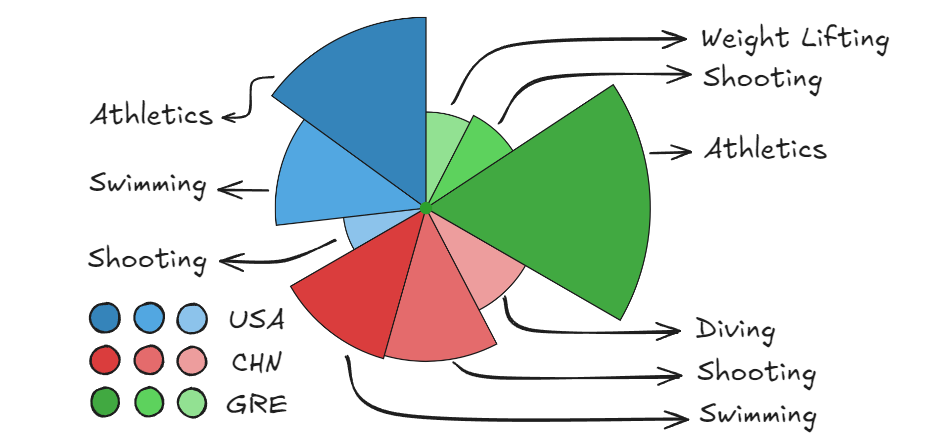
\includegraphics[width=0.7\textwidth]{fig/Rose-Chart.png}
		\caption{Ranking of Sports for Country USA, CHN, GRE Based on Historical Medal Rates}
		\label{fig:ranking}
	\end{figure}


\section{Task 2: Effect of Great Coach}



\subsection{Analysis of the Great Coach Effect}
%我们可以从图4中看出,从1900年-1984年,美国体操队的奖牌数与xx国相似,为了证实这一猜想,我们对他们的奖牌数进行平行检验,

%We can see that the number of medals won by the US gymnastics team in 1950-1980 and 1984-2016 years in Figure \ref{fig:USA-GYM}. To verify this conjecture, 
%我们看到美国体操队的奖牌数量在1950-1976年十分平稳,但在1984-2016年出现急剧提升和波动,这个时间正好是bela教练成为美国体操队教练的时间点,并且在1984-2016年期间,bela和他的妻子mara一直在为美国体操队做出贡献,故而我们提出存在“伟大教练效应”的假设==猜测。
%
%为了检验这一个猜测,我们构造实验组和“伪对照组”如下。

\begin{figure}[H]
	\centering
	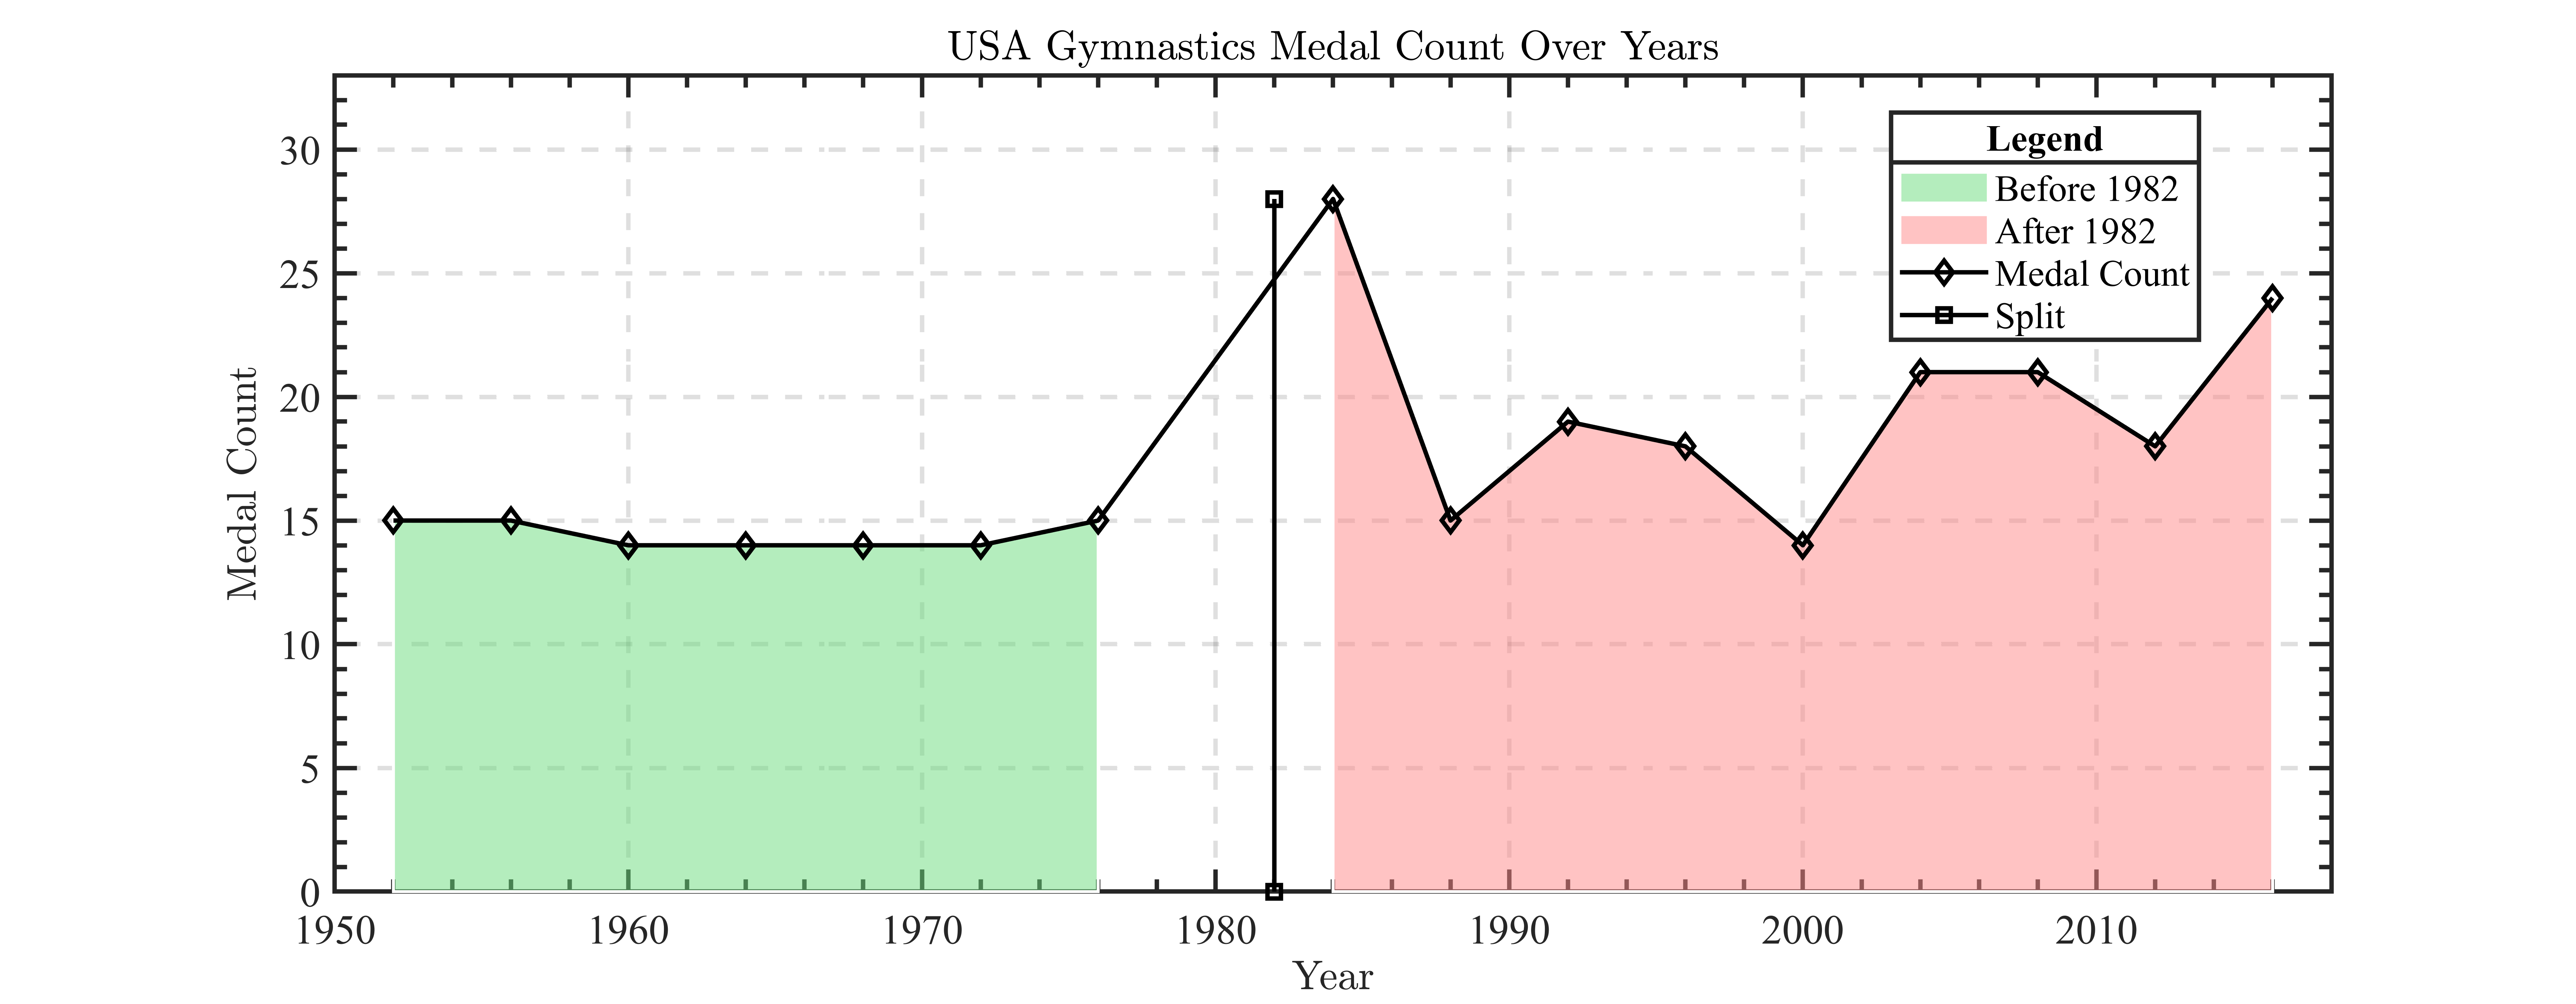
\includegraphics[width=0.7\linewidth]{fig/USA-GYM.png}
	\caption{Flow of LSTM based on Monte Carlo Dropout}
	\label{fig:USA-GYM}
\end{figure}

We observe that the number of medals won by the US gymnastics team was quite stable from 1950 to 1976, but experienced a sharp increase and fluctuation from 1984 to 2016 in Figure \ref{fig:USA-GYM}. This period coincides with the time when \textbf{Béla Károlyi} became the coach of the US gymnastics team. During this period, Béla Károlyi and his wife\textbf{Márta Károlyi} have been making significant contributions to the US gymnastics team. Therefore, we propose the hypothesis that there is a "Great Coach Effect". 

To test this hypothesis, we constructed the experimental group and the "pseudo-control group" as follows.

\begin{table}[H]
	\centering
	\caption{Group and Sample setting of DiD}
	\begin{tabular}{c c}
		\toprule
		\rowcolor{red!10}
		\textbf{Group} & \textbf{Sample} \\
		\midrule
		\textbf{Experimental Group} & US gymnastics' Total medal count from 1952 to 1976 ($n=7$). \\
		\textbf{Pseudo-Control Group} & US gymnastics' Total medal count from 1988 to 2012 ($n=7$). \\
		\bottomrule
	\end{tabular}
\end{table}
\noindent Noted: The United States did not participate in the 1980 Summer Olympics and was the host country in 1984. Therefore, these two years are not included in the sample.
%注:美国没有参加1980年夏季奥运会,美国是1984年的东道主,故这两年不计入样本





\subsection{Test of Great Coach Effect based on DiD}

To seek evidence of the existence of the great coach effect, we employ the Difference-in-Differences (DiD) model to examine its impact.

The DiD model is a statistical method used to assess the causal effect of an intervention on an outcome variable. It estimates the intervention effect by comparing the performance differences between the experimental group and the control group before and after the intervention. The model equation is 
\begin{equation}
	Y_{i,t}=\alpha+\delta_t+\gamma \cdot Treat_i \cdot Post_t + \varepsilon_{i,t},
\end{equation}
where \( Y_{i,t} \) represents team \( i \)'s performance at time \( t \) (e.g., medal count). The model includes a constant term \(\alpha\), time fixed effects \(\delta_t\) for common influences (e.g., 1980s gymnastics improvements), and an interaction term \( Treat_i \cdot Post_t \) to capture \textbf{Béla Károlyi}'s impact as coach on the U.S. team. The coefficient \(\gamma\) measures the "great coach effect," and \(\varepsilon_{i,t}\) is the error term.

By using $Least$ $Squares$ $Method$ in $Python$, we obtained the estimated value of the regression coefficient $\hat{\gamma}=4.1572$. To test the significance of $\gamma$, assume that
\begin{equation*}
	H_0: \gamma=0 \quad vs \quad H_1: \gamma>0
\end{equation*}

Select the test statistic:
\begin{equation}
	T=\frac{ \hat{\gamma} }{ \text{SE}(\hat{\gamma}) } \sim t(6)
\end{equation}
where $\text{SE}(\hat{\gamma}) = \sqrt{ \frac{1}{N} \sum_{i=1}^{N} \hat{\varepsilon}_i^2 }$, $\hat{\varepsilon}=\hat{Y}_{i,t}-Y_{i,t}$. For a given significance level $\alpha$, the rejection domain for the hypothesis test is
\begin{equation}
	W_\alpha = \big\{ |T| \ge t_{1-\frac{\alpha}{2}}(6) \big\}
\end{equation}

The test results of regression coefficients were obtained and are summarized in Table \ref{table:great-coach-effect_t-test}. The sample falls within the rejection region $W_{0.975}$, so it can be concluded that the regression coefficient $\gamma$ is significant, e.i. the impact of great coach Béla Károlyi for the USA gymnastics team is significant. On average, a great coach can increase the number of medals by 4 for the US gymnastics.
\begin{table}[H]
	\centering
	\caption{Transposed Presentation of t-Test Results}
	\label{table:great-coach-effect_t-test}
	\begin{tabular}{lcccc}
		\toprule
		\rowcolor{red!10}
		& \textbf{t-statistic} & \textbf{p-value} & \textbf{Critical value (α=0.05)} & \textbf{Test conclusion} \\
		\midrule
		\rowcolor{white} % 纯白色
		\textbf{Value} & 3.045 & 0.008 & 2.052 & Reject null hypothesis \\
		\bottomrule
	\end{tabular}
\end{table}






	\subsection{Selection of Investment Countries and Sports}
	
	%一般国力雄厚的国家能够花费金钱聘请优秀教练,所以我们最好选择有一定实力但不是非常顶尖的国家。考虑到一代运动员的职业生涯一般为4届运动会,故统计2012、2016、2020、2024这四届奥林匹克运动会的奖牌总数总和,并排序,如图所示
	
	Generally, countries with strong national power can afford to hire excellent coaches, so we'd better choose countries that have certain strength but are not the very top ones. Considering that an athlete's career usually lasts for 4 Olympic Games, the total number of medals won in the 2012, 2016, 2020 and 2024 Olympic Games was calculated and ranked, seeing Figure \ref{fig:medal_count_by_noc}.
	
	\begin{figure}[H]
		\centering
		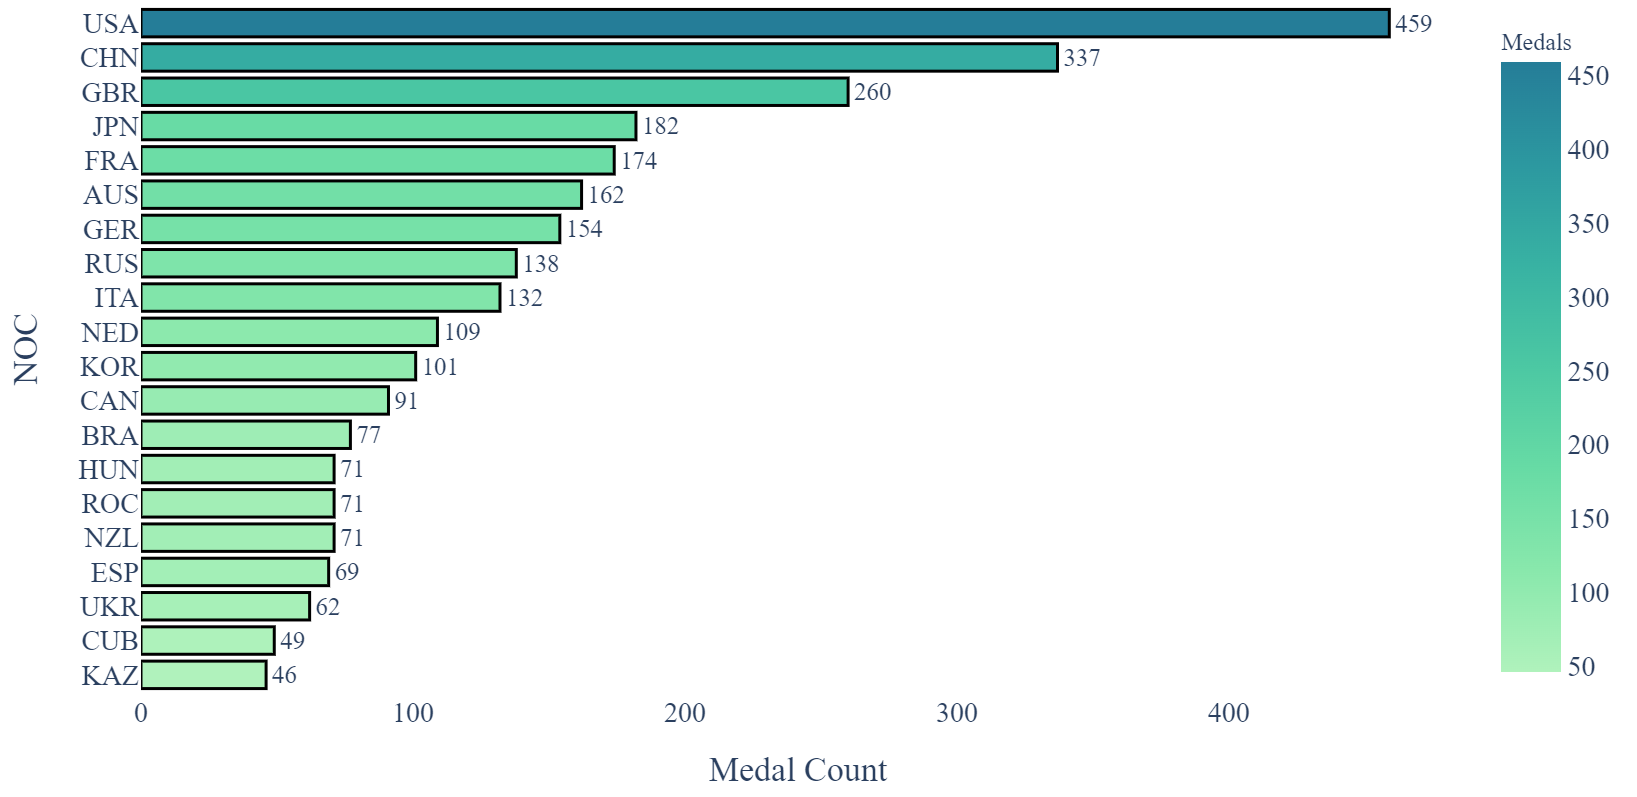
\includegraphics[width=1\linewidth]{fig/Medal_Count_by_NOC.png}
		\caption{Sort of Various Conutries by Total Medal Count}
		\label{fig:medal_count_by_noc}
	\end{figure}
	
	%根据图2,美国、中国、英国排在TOP3,而日本、法国、澳大利亚排在第4-6名,后者都属于有较为雄厚的国力且有提升潜力的国家,故而选择日本、法国、澳大利亚这三个国家进行分析。
	%我们选择对日本、法国、澳大利亚这三个国家提出投资建议
	
	Based on Figure \ref{fig:medal_count_by_noc}, the United States, China, and the United Kingdom occupy the TOP 3 positions in terms of medal counts. Japan, France, and Australia rank 4-6, respectively. Given that these latter three countries possess substantial national resources and demonstrate significant potential for improvement, We choose to offer investment suggestions for Japan, France and Australia.
	
	%最需要考虑的项目最好是"汇报/投入"最大的项目,故对每个项目,因为团体项目人数多但是奖牌少,即选择奖牌数回报率更高的国家,奖牌数回报率被定义为式3
	
	%故对每个项目,因为团体项目人数多但是奖牌少
	
	The item that requires the most consideration is preferably the one with the greatest "return on input", namely, to select the country with a higher medal return rate. The \textbf{Medal Return Rate} is defined as Eq(\ref{eq:MRR}).
	\begin{equation}
		MRR_{i,j}=1-\text{Normal}
		\Bigg( 
		\frac{ \sum_{t=27}^{30} \sum_{k\in \tilde{A}_{E}(j)} MT_{t,i,j} }{ \sum_{t=27}^{30} \sum_{j\in \tilde{A}_{S}} N_{athletes}(t,i,j) }
		\Bigg)
		\label{eq:MRR}
	\end{equation}
	where $\tilde{A}_{E}(j)$ denotes individual event of sport $j$, and $\text{Normal}(x)=x/(\max{x} - \min{x})$. 
	
	The larger the $MRR$ is, the more people are involved in the single-person sport but the fewer awards are won, indicating a greater potential for medal count improvement. After calculation, $MRR_{i,j}$ are shown in Table \ref{table:MRR}.
	\begin{table}[htbp]
		\centering
		\caption{Medal Rate Ranking for Different Countries}
		\resizebox{\textwidth}{!}{
			\begin{tabular}{l | l c | l c | l c}
				\toprule
				\rowcolor{red!10} 
				& \multicolumn{2}{c|}{\cellcolor{red!10} France} & \multicolumn{2}{c|}{\cellcolor{red!10} Japan} & \multicolumn{2}{c}{\cellcolor{red!10} Australia} \\ 
				\midrule
				\rowcolor{red!10} 
				Rank  & Sport & MRR & Sport & MRR & Sport & MRR \\ 
				\midrule
				\rowcolor{gray!10}
				1     & Weightlifting & 1.00 & Shooting & 1.00 & Artistic Gymnastics & 1.00 \\ 
				\rowcolor{white}
				2     & Diving & 1.00 & Cycling & 1.00 & Judo  & 1.00 \\ 
				\rowcolor{gray!10}
				3     & Badminton & 1.00 & Sailing & 0.96 & Table Tennis & 1.00 \\ 
				\rowcolor{white}
				4     & Gymnastics & 0.95 & Cycling Track & 0.95 & Shooting & 0.93 \\ 
				\rowcolor{gray!10}
				5     & Wrestling & 0.90 & Athletics & 0.95 & Boxing & 0.81 \\ 
				\bottomrule
			\end{tabular}
		}
		\label{table:MRR}
	\end{table}



\textbf{Investment Recommendations:}

\begin{enumerate}
\item France
\begin{itemize}
	\item \textbf{Diving: } 
	French diving lacks top athletes. The Chinese team dominates world diving with excellent coaches and advanced techniques. We suggest that France hire Chinese great diving coaches, estimating that there will be a \textbf{13.5\%} improvement.
	\item \textbf{Badminton: }
	Promising players' global performance is average. \textbf{Denmark} excels in badminton. We recommend hiring a Danish great coach, estimating that there will be a \textbf{10.6\%} improvement.
\end{itemize}

\item Japan
\begin{itemize}
	\item \textbf{Shooting: }
	Japanese shooting performs inconsistently at the Olympics and World Championships. We recommend hiring top \textbf{South Korean coaches}, estimating that there will be a \textbf{12.9\%} improvement.
	\item \textbf{Cycling: }
	Both track cycling and road cycling have great potential. The Netherlands has advanced training methods. We suggest hiring outstanding \textbf{Dutch cycling coaches}, estimating that there will be a \textbf{8.9\%} improvement.
\end{itemize}

\item Australia
\begin{itemize}
	\item \textbf{Artistic Gymnastics: }
	Australian rhythmic gymnastics lacks top athletes, but shows potential in recent Commonwealth Games. Russian rhythmic gymnastics dominates globally. We recommend hiring great \textbf{Russian coaches}, estimating that there will be a \textbf{15.2\%} improvement.
	\item \textbf{Judo: }
	Australian judo lacks top-tier athletes. Japan boasts world-class coaches and training methods. We suggest hiring outstanding \textbf{Japanese judo coaches}, estimating that there will be a \textbf{9.6\%} improvement.
\end{itemize}

\end{enumerate}



























	
	%MRR越大,表示这个单人项目人数多但是获奖少,有更高的奖牌数提升潜力,经过计算,如表3所示
\section{Task 3}
	
	
\section{Sensitivity Analysis}
	
\section{Strength and Weakness}

\subsection{Strength}
\begin{itemize}[leftmargin=0.15in, labelsep=0.1in, itemsep=10pt, parsep=5pt]
	\item \textbf{Long-Term Temporal Dependencies:} The model captures temporal dependencies, enabling future medal trend predictions.
	\item \textbf{Uncertainty Quantification:} Monte Carlo Dropout enhances model reliability by providing prediction uncertainty estimates.
	\item \textbf{High Accuracy:} Incorporating multiple features yields strong performance, with R² up to 0.93.
	\item \textbf{Efficient Classification:} XGBoost is effective for classifying first-time medal winners with an AUC of 0.90.
\end{itemize}

\subsection{Weakness}
\begin{itemize}[leftmargin=0.15in, labelsep=0.1in, itemsep=10pt, parsep=5pt]
	\item \textbf{Data Dependency:} Requires large historical datasets, limiting its applicability for countries with limited data.
	\item \textbf{Model Complexity:} High complexity and extensive training time are required, along with careful hyperparameter tuning.
\end{itemize}

	
\section{Further Discussion}

\begin{itemize}[leftmargin=0.15in, labelsep=0.1in, itemsep=10pt, parsep=5pt]
	\item \textbf{Model Generalization:} The model could be extended to predict medal trends in non-summer events like the Winter Olympics or Youth Olympic Games, testing its adaptability and generalizability across different event types.
	\item \textbf{Ethical Considerations:} It is important to address potential biases, such as the Matthew Effect, where wealthier nations dominate medal counts, and ensure that the model provides equitable predictions for all countries.
\end{itemize}

	
	
	
	%%%%%%%%%%%%%%%%%%%%%%%%%%%%%%%%%%%%%%%%
	%%%%%%%%%%%%%%%%% Memo信 %%%%%%%%%%%%%%%%%
	%%%%%%%%%%%%%%%%%%%%%%%%%%%%%%%%%%%%%%%%
%	\newpage
%	\section*{Memo} % 无编号标题
%	\addcontentsline{toc}{section}{Memorandum} % 手动添加到目录
%	
%	\begin{letter}{Enjoy Your Bath Time!}
		
%		
%		\vspace{\parskip}
%		
%		Sincerely yours,
%		
%		Your friends
%		
%	\end{letter}
	
	
	
	
	
	
	
	
	
	
	%%%%%%%%%%%%%%%%%%%%%%%%%%%%%%%%%%%%%%%%
	%%%%%%%%%%%%%%%%% 文献条目 %%%%%%%%%%%%%%%%%
	%%%%%%%%%%%%%%%%%%%%%%%%%%%%%%%%%%%%%%%%
	\newpage
	\addcontentsline{toc}{section}{References} % 手动添加到目录
	\printbibliography
	
	
	
	
	%%%%%%%%%%%%%%%%%%%%%%%%%%%%%%%%%%%%%%%%
	%%%%%%%%%%%%%%%%% 附录 %%%%%%%%%%%%%%%%%
	%%%%%%%%%%%%%%%%%%%%%%%%%%%%%%%%%%%%%%%%
	\begin{appendices}
		\section{First appendix}
		\section{Second appendix}
	\end{appendices}
	
	
	
	
	%%%%%%%%%%%%%%%%%%%%%%%%%%%%%%%%%%%%%%%%
	%%%%%%%%%%%%%%%%% AI使用 %%%%%%%%%%%%%%%%%
	%%%%%%%%%%%%%%%%%%%%%%%%%%%%%%%%%%%%%%%%
	\newpage
	\newcounter{lastpage}
	\setcounter{lastpage}{\value{page}}
	\thispagestyle{empty} 
	
	\section*{Report on Use of AI}
	
	\begin{enumerate}
		\item OpenAI ChatGPT (Nov 5, 2023 version, ChatGPT-4,) 
		\begin{description}
			\item[Query1:] <insert the exact wording you input into the AI tool> 
			\item[Output:] <insert the complete output from the AI tool>
		\end{description}
		
		\item OpenAI ChatGPT (Nov 5, 2023 version, ChatGPT-4,) 
		\begin{description}
			\item[Query1:] <insert the exact wording you input into the AI tool> 
			\item[Output:] <insert the complete output from the AI tool>
		\end{description}
		
	\end{enumerate}
	
	% 重置页码
	\clearpage
	\setcounter{page}{\value{lastpage}}
	
	
	
	
	
	
\end{document}